\documentclass[%
	11pt,
	a4paper,
	utf8,
	%twocolumn
		]{article}	

\usepackage{style_packages/podvoyskiy_article_extended}


\begin{document}
\title{Пояснительная записка\\{\large Вычислительные техники решения задач линейного программирования в частично-целочисленной постановке и приемы работы с решателем SCIP}}

\author{\itshape Подвойский А.О., Глазунова Е.В.}


\date{}
\maketitle

\thispagestyle{fancy}

%Здесь приводятся заметки по специальным вопросам теории оптимизации

%\shorttableofcontents{Краткое содержание}{1}

\tableofcontents

\section{Ключевые термины и определения}

\emph{Сценарий} -- это математическая постановка задачи, описанная в терманах математического программирования (например, линейного)

\emph{Сценарий обучающего поднабора} -- это сценарий из коллекции сценариев, которые используются на {обучающей фазе} алгоритма машинного обучения

\emph{Сценарий тестового поднабора} -- это сценарий, который используется {для построения прогноза} с помощью алгоритма машинного обучения

\section{Полезные ресурсы}

\url{http://plato.asu.edu/sub/benchm.html} Сравнительный анализ эффективности различных решателей от H. D. Mittelmann

\section{LP- и MPS-форматы математической постановки}

\href{https://support.gurobi.com/hc/en-us/articles/360013420131-What-are-the-differences-between-LP-and-MPS-file-formats-}{MPS, LP. Блок Gurobi}

LP-формат спроектирован таким образом, чтобы его было удобно читать человеку. Например, Gurobi в LP-формате записывает коэффициенты с меньшей точностью. Кроме того {\color{red}LP-формат \emph{не гарантирует} сохранение порядка переменных (!)}. В результате траектория поиска решения от запуска к запуску может изменяться. LP-формат имеет смысл использовать для проверки корректности модели.

MPS-формат записывается коэффициенты с полной точностью, \emph{сохраняя порядок следования переменных}. 


\section{Кратко о MPS-формате представления математической постановки задачи}

Больше деталей по ссылке \url{https://www.gurobi.com/documentation/9.5/refman/mps_format.html}

MPS-формат -- это старейший формат представления математчиских постановок. Различают два вида этого формата: фиксированный и свободный. В фиксированном формате под имя строки и столбца отводится ровно 8 символов (пробел считается частью имени), а в свободном формате имена могут иметь произвольную длину.

Строки, которые начинаются с символа \verb|*| считаются комментариями.

Получить все секции MPS-файла можно так
\begin{lstlisting}[
style = bash,
numbers = none
]
$ cat problem.mps | grep -nE "^[A-Z]{2,}.*$" > res.txt
$ cat res.txt
# 5:NAME          problem.mps
# 6:OBJSENSE
# 8:ROWS
# 158077:COLUMNS
# 621330:RHS
# 700365:BOUNDS
# 903714:ENDATA
\end{lstlisting}

\subsection{Секция \texttt{NAME}}
Первая секция в MPS-файле называется \verb|NAME|. Она задает имя модели. В фиксированном формате имя модели начинается в 15 столбце.

\subsection{Секция \texttt{OBJSENSE}}

Следующая (необязательная) секция \verb|OBJSENSE| указывает направление оптимизации (задача решается на минимум или на максимум).

\subsection{Секция \texttt{ROWS}}

В секции \verb|ROWS| каждая строка описывает \emph{тип ограничения} (\verb|E| -- равенство, \verb|L| -- меньше-или-равно, \verb|G| -- больше-или-равно) и \emph{имя ограничения}. \verb|N| указывает на целевую функцию.

Самая большая секция MPS-файла это секция \verb|COLUMNS|, в которой описываются переменные с ненулевыми коэффициентами
\begin{lstlisting}[
style = bash,
basicstyle = \fontsize{8pt}{8pt}\ttfamily,
numbers = none
]
...
COLUMNS
    z_balance_plus_0_177360  z_balance_0_177360                           1  Obj                                          3
    z_balance_plus_100_177446  z_balance_100_177446                         1  Obj                                          3
    z_balance_plus_101_177488  Obj                                          3  z_balance_101_177488                         1
    z_balance_plus_102_177447  z_balance_102_177447                         1  Obj                                          3
...
\end{lstlisting}

Первая строка говорит, что переменная \verb|z_balance_plus_0_177360| входит в ограничение

\noindent\verb|z_balance_0_177360| с коэффициентом 1, а в целевую функцию -- с коэффициентом 3.

\subsection{Секция \texttt{COLUMNS}}

Секция \verb|COLUMNS| может дополнительно включать маркеры целочисленности. Переменные, расположенные между парой маркеров должны принимать целочисленные значения. Все переменные эти переменные по умолчанию имеют нижнюю границу 0 и верхнюю границу 1. Если требуется задать другие значения нижних и верхних границ, то это можно сделать в секции \verb|BOUNDS|.
\begin{lstlisting}[
style = bash,
basicstyle = \fontsize{8pt}{8pt}\ttfamily,
numbers = none
]
  INTSTART              'MARKER'                                        'INTORG'  *начало секции
    y_tu_170_177684_9_10  out_throughput_vs_units_9                         1  cdo_lower_1_2112221020_1_9_10                         1
    y_tu_170_177684_9_10  static_load_terminal_170_177684_9_10                    665600  multiplicity_of_fronts_284                         1
    y_tu_170_177684_9_10  cdo_upper_1_2112221020_1_9_10                         1  Obj                                          0
    y_tu_170_177685_9_10  cdo_upper_1_2112221020_1_9_10                         1  cdo_lower_1_2112221020_1_9_10                         1
...
    y_tu_9_177398_11_9    cdo_lower_1_251194210_1_11_9                         1  multiplicity_of_fronts_345                         1
    y_tu_9_177398_11_9    cdo_upper_1_251194210_1_11_9                         1  static_load_terminal_9_177398_11_9                    540200
    y_tu_9_177398_11_9    out_throughput_vs_units_8                         1  Obj                                          0
   INTEND                'MARKER'                                        'INTEND' *конец секции
\end{lstlisting}

Здесь \verb|INTSTART| -- это имя маркера (игнорируется), \verb|'MARKER'| -- специальная строка (в одинарных ковычках), \verb|'INTORG'| -- начало целочисленной секции и \verb|'INTEND'| -- конце целочисленной секции.

\subsection{Секция \texttt{RHS}}

Следующая секция \verb|RHS| (right-hand side) MPS-файла описывает правую часть ограничения
\begin{lstlisting}[
style = bash,
numbers = none	
]
RHS                   cdo_lower_1_2414112504_1_3_3                         4  cdo_lower_1_2414112504_1_3_30                         4
# cdo_lower_1_2414112504_1_3_3: +1 y_tu_170_177743_3_3 +1 y_tu_170_177744_3_3 >= +4
# cdo_lower_1_2414112504_1_3_30: +1 y_tu_170_177743_3_30 +1 y_tu_170_177744_3_30 >= +4
\end{lstlisting}

\subsection{Секция \texttt{BOUNDS}}

Это необязательная секция. По умолчанию каждая переменная имеет нижнюю границу 0 и бесконечную верхнюю границу. Каждая строка этой секции может изменять нижнюю границу, верхнюю границу или обе границы переменной. 

Поддерживаются следующие типы:
\begin{itemize}
	\item \verb|LO|: нижняя граница,
	
	\item \verb|UP|: верхняя граница,
	
	\item \verb|FX|: переменная, зафиксированная в какое-то конкретное значение,
	
	\item \verb|FR|: свободная переменная (без верхней и нижней границы),
	
	\item \verb|MI|: бесконечная нижняя граница,
	
	\item \verb|PL|: бесконечная верхняя граница,
	
	\item \verb|BV|: бинарная переменная (0 или 1),
	
	\item \verb|LI|: нижняя граница для целочисленной переменной,
	
	\item \verb|UI|: верхняя граница для целочисленной переменной,
	
	\item \verb|SC|: верхняя граница для полунепрерывной переменной,
	
	\item \verb|SI|: верхняя граница для полуцелочисленной переменной.
\end{itemize}






\section{Ключевые компоненты платформы SCIP}

\subsection{Решатель SCIP. Общие сведения}

SCIP (Solving Constraint Integer Programs) \url{https://www.scipopt.org/} -- решатель, предназначенный для решения задач \emph{линейного} и \emph{нелинейного} программирования в частично-целочисленной постановке.

\subsubsection{Установка решателя SCIP}
Решатель проще всего установить вместе с оберткой PySCIPOpt \url{https://github.com/scipopt/PySCIPOpt} с помощью менеджеров \texttt{pip} или \texttt{conda}
\begin{lstlisting}[
style = bash,
numbers = none
]
# установить последнюю доступную версию SCIP
$ pip install pyscipopt
$ conda install -c conda-forge pyscipopt
# установить заданную версию SCIP
$ conda install -c conda-forge pyscipopt=3.4.0
\end{lstlisting}

В ноябре 2023 вышла новая исправленная версия SCIP 8.1.0, но она показывает низкую производительность относительно версии SCIP 8.0.3, поэтому рекомендуется ставить отдельно SCIP и отдельно PySCIPOpt
\begin{lstlisting}[
style = bash,
numbers = none
]
$ conda install -c conda-forge scip==8.0.3 
$ conda install -c conda-forge pyscipopt
\end{lstlisting}

\subsubsection{Приемы работы с решателем SCIP в интерактивной оболочке \texttt{scip}}

Для того чтобы сделать логи более подробными следует включить следующие строки в конфигурационный файл SCIP
\begin{lstlisting}[
title = {\sffamily scip.set},
style = bash,
numbers = none
]
...
display/lpinfo = TRUE
display/ninfeasleaves/active = 2
display/allviols = TRUE
\end{lstlisting}

\subsubsection{Приемы работы с решателем SCIP через обертку PySCIPOpt}

Работа над задачей начинается с создания пустого экземпляра модели
\begin{lstlisting}[
style = ironpython,
numbers = none
]
import pyscipopt

model = pyscipopt.Model()
\end{lstlisting}

На созданном экземпляре можно вызывать методы чтения модели, конфигурационного файла параметров решателя и т.д.
\begin{lstlisting}[
style = ironpython,
numbers = none,
]
model.readProblem("./problem.lp")
model.readParams("./scip.set")
...
\end{lstlisting}

С расшифровкой параметров таблицы логов (например, \verb|strbr| или \verb|mdpt|) можно познакомится на странице проекта GAMS \url{https://www.gams.com/latest/docs/S_SCIP.html}.

Получить коллекцию ограничений в виде списка словарей, содержащих имя переменной и коэффициент при ней в ограничении, можно так
\begin{lstlisting}[
style = ironpython,
numbers = none
]
model = pyscipopt.Model()
model.readProblem("...")

all_conss: t.Iterable[dict] = [model.getValsLinear(cons) for cons in model.getConss()]
"""
all_conss = [
    {  # cons-1
    	'cm_or_0_1_1': -1.0,
    	'cooked_mass_0_1_1': 1.0,
    	'passport_0_1_1': -1.0
    },
    {  # cons-2
    	'cm_or_0_1_10': -1.0,
    	'cm_or_0_1_9': 1.0,
    	'cooked_mass_0_1_10': 1.0,
    	'passport_0_1_10': -1.0
    },
    ...
]
"""
\end{lstlisting}



\subsection{Декомпозиционный решатель GCG. Общие сведения}

GCG \url{https://gcg.or.rwth-aachen.de/#about} -- это универсальный декомпозиционный решатель для задач линейного программирования в частично-целочисленной постановке, расширающий возможности базового решателя SCIP.

Он выявляет структуры в модели, к которым могут быть применены \emph{переформулировка Данцига-Вольфе} или \emph{декомпозиция Бендера}.

Модфицированная постановка задачи (после переформулировки Данцига-Вольфе) решается с помощью обобщения метода ветвей-и-границ, а именно с помощью метода ветвей-штрафов-секущих (branch-price-and-cut), включающего различные механизмы поиска решения -- превичные эвристики, стратегии ветвления, стратегии стабилизации, стратегии назначения штрафов и пр.

\subsubsection{Установка решетеля GCG}

Проще всего решатель установить вместе с обреткой PyGCGOpt \url{https://github.com/scipopt/PyGCGOpt} с помощью мендежера пакетов \texttt{conda}
\begin{lstlisting}[
style = bash,
numbers = none
]
$ conda install -c conda-forge pygcgopt
\end{lstlisting}



\subsubsection{Приемы работы с решателем GCG в интерактивной оболочке \texttt{gcg}}

Прочитать постановку задачи
\begin{lstlisting}[
style = bash,
numbers = none
]
GCG> read problem.lp
\end{lstlisting}

Запустить процедуру редуцированния размерности
\begin{lstlisting}[
style = bash,
numbers = none
]
GCG> presolve
\end{lstlisting}

Запустить процедуру поиска структур в матрице ограничений
\begin{lstlisting}[
style = bash,
numbers = none
]
GCG> detect
\end{lstlisting}

Записать постановку задачи сниженной размерности для \texttt{gnuplot}
\begin{lstlisting}[
style = bash,
numbers = none
]
GCG> write problem problem_reduced.gp
\end{lstlisting}

Фрагмент gp-файла
\begin{lstlisting}[
style = bash,
numbers = none
]
set encoding utf8
set terminal pdf
set output "problem_reduced.pdf"
set xrange [-1:506441]
set yrange[347788:-1]
set object 1 rect from 0,0 to 506441,183384 fc rgb "#1340C7"
set object 3 rect from 163304,183384 to 163306,183385 fc rgb "#718CDB" 
set object 4 rect from 163306,183385 to 163308,183386 fc rgb "#718CDB" 
set object 5 rect from 163308,183386 to 163310,183387 fc rgb "#718CDB" 
set object 6 rect from 163310,183387 to 163312,183388 fc rgb "#718CDB" 
set object 7 rect from 163312,183388 to 163314,183389 fc rgb "#718CDB" 
set object 8 rect from 163314,183389 to 163316,183390 fc rgb "#718CDB" 
set object 9 rect from 163316,183390 to 163318,183391 fc rgb "#718CDB" 
set object 10 rect from 163318,183391 to 163320,183392 fc rgb "#718CDB" 
set object 11 rect from 163320,183392 to 163322,183393 fc rgb "#718CDB" 
...
\end{lstlisting}

Создать pdf-файл декомпозиции задачи после шага снижения размерности
\begin{lstlisting}[
style = bash,
numbers = none
]
$ gnuplot problem_reduced.gp
\end{lstlisting}

\subsubsection{Приемы работы с решателем GCG через обертку PyGCGOpt}

\section{Выявленные баги SCIP и тонкости процедуры поиска решения}

\subsection{Недопустимое решение для релаксированной постановки задачи}

По состоянию на 18.06.2022 г. решатель SCIP версии 8.0.0 с оберткой PySCIPOpt версий 4.0.0 и 4.2.0 для операционной системы Windows 10 \emph{релаксированную постановку задачи} (т.е. при снятых ограничениях на целочисленность переменных) оценивает как неспособную привести к допустимому решению.

SCIP версии 7.0.3 (PySCIPOpt 3.4.0) как на операционной системе Windows 10, так и на Unix-подобных операционных системах (в частности, MacOS Monterey 12.1 и Linux Centos 7) решает задачу в релаксированной постановке корректно.

Однако можно попробовать <<помочь>> SCIP 8.0.X справится с численными проблемами следующим образом

\noindent\url{https://stackoverflow.com/questions/24702747/scip-infeasibility-detection-with-a-minlp}
\begin{lstlisting}[
title = {\sffamily scip.set},
style = bash,
numbers = none,
]
numerics/epsilon = 1e-07  # default 1e-09
numerics/feastol = 1e-05  # default 1e-06
numerics/sumepsilon = 1e-05  # default 1e-06
\end{lstlisting}

\subsection{Неединственность релаксированного решения}

Если эвристические приемы строятся на базе релаксированного решения задачи, важно помнить, что релаксированные решения, полученные с помощью различных решателей с точки зрения распределения значений переменных могут существенно различаться\footnote{Потому как гиперплоскость целевой функции может касаться политопа не в вершине, а по грани}, не смотря на то, что во всех случах зазор будет нулевым и целевая функция будет имееть одно и тоже значение (с оговоркой на допуск точности решателя). 

\subsection{Замечание о стабильности работы решателя SCIP на различных операционных системах}

\begin{itemize}
	\item Вычислительные эксперименты проводились на трех версиях решателя SCIP (7.0.0, 7.0.3, 8.0.0) и трех платформах: Windows~10, MacOS (Monterey~12), Linux (Centos~7). Разброс времени поиска решения для каждой конфигурации решателя оценивается минимум по 3 запускам сценария
	
	\item На текущий момент наиболее стабильные и наиболее адекватные результаты получаются
	\begin{itemize}
		\item для ОС Linux (Centos 7) и ОС MacOS (Monterey12) на решателе SCIP версии 7.0.3 (обертка PySCIPOpt 3.4.0) и платформе Ecole версии 0.7.3 , собранных для однопоточной реализации
		
		\item для ОС Windows 10 на решателе SCIP версии 8.0.0 (обертка PySCIPOpt 4.0.0), собранном для однопоточной реализации
	\end{itemize}
	
	\item Последняя доступная версия решателя SCIP 8.0.0 (PySCIPOpt 4.1.0) на MacOS (Monterey 12.1) и Linux (Centos 7) при тех же настройках, что и для SCIP версии 7.0.3, как правило, работает значительно медленнее (2.5-2.85 раза) и в большинстве случаев либо не успевает найти решение за отведенное время, либо «просаживает» целевую функцию
\end{itemize}

\subsection{Чтение/запись lp-фалов и порядок следования переменных}

Чтение/запись файла математической постановки изменяет порядок следования переменных в целевой функции, что может непредсказуемо влиять на эффективность процедуры поиска решения. Если после модификации проблемы с помощью например фиксации нулей сразу запустить процедуру поиска, то будут одни результаты пресолвинга и картина поиска решения, а если модифицированную постановку записать и снова прочитать, то -- другие. Причем последствия могут быть очень серьезными: в одном случае решение находится за 20 минут, в другом -- за 3 часа. Какой порядок следования переменных <<правильный>>?

\section{Альтернативные решатели с открытым исходным кодом}

\subsection{Решатель HIGHS}

\subsubsection{Установка решателя на Centos 7}

Установить решатель HIGHS \url{https://ergo-code.github.io/HiGHS/get-started.html} можно следующим образом
\begin{enumerate}
	\item Скачать репозиторий проекта
\begin{lstlisting}[
style = bash,
numbers = none
]
$ git clone https://github.com/ERGO-Code/HiGHS.git
\end{lstlisting}
    \item Установить \texttt{cmake} версии \texttt{>=3.15}
\begin{lstlisting}[
style = bash,
numbers = none
]
# https://cmake.org/download/
$ wget https://github.com/Kitware/CMake/releases/download/v3.24.2/cmake-3.24.2.tar.gz
$ tar -xvf cmake-3.24.2.tar.gz
$ cd cmake-3.24.2
$ ./bootstrap --prefix=/usr --datadir=share/cmake --docdir=doc/cmake && make
$ sudo make install
$ cmake --version  # cmake version 3.24.2
\end{lstlisting}
    \item Установить альтернативную версию комилятора \texttt{gcc} (например, версии 7) для сборки проекта
\begin{lstlisting}[
style = bash,
numbers = none	
]
# https://linuxize.com/post/how-to-install-gcc-compiler-on-centos-7/
$ gcc --version  # gcc (GCC) 4.8.5 20150623 (Red Hat 4.8.5-36)
\end{lstlisting}

Чтобы получить доступ к альтернативной версии компилятора GCC 7, требуется запустить новый сеанс командной оболочки с помощью утилиты \texttt{scl}
\begin{lstlisting}[
style = bash,
numbers = none
]
$ scl enable devtoolset-7 bash
# или для ZSH
# scl enable devtoolset-7 zsh
$ gcc --version  # gcc (GCC) 7.3.1 20180303 (Red Hat 7.3.1-5)
\end{lstlisting}

    \item В директории проекта \texttt{HIGHS} создать поддиректорию \texttt{build} и запустить из-под нее утилиту \texttt{cmake}
\begin{lstlisting}[
style = bash,
numbers = none
]
$ cd HiGHS
$ mkdir build
$ cd build
$ cmake -DFAST_BUILD=ON ..
$ cmake --build .
# Чтобы убедится в том, что сборка прошла успешно, рекомендуется запустить быстрые тесты
$ ctest
\end{lstlisting}

В результате будет создан исполняемый файл \texttt{build/bin/highs}
    
    \item Добавить путь до утилиты в конфигурационный файл оболочки
\begin{lstlisting}[
title = {\sffamily .zshrc},
style = bash,
numbers = none
]
...
export PATH=${HOME}/Projects/HiGHS/build/bin:$PATH
\end{lstlisting}

После внесения изменений в конфигурационный файл, можно перечитать конфигурацию сессии
\begin{lstlisting}[
style = bash,
numbers = none
]
$ source .zshrc
\end{lstlisting}
\end{enumerate}
\vspace*{3mm}

\subsubsection{Приемы работы с решателем}

Для запуска решателя в MILP-режиме требуется только передать путь до \texttt{*.lp/*.mps}-файла
\begin{lstlisting}[
style = bash,
numbers = none
]
$ highs /path/to/model.lp
$ highs --help
\end{lstlisting}

Для запуска решателя в режиме поиска релаксированного решения требуется параметру \verb|--solver| передать название метода (на текущий момент поддерживается только симплекс-метод \texttt{simplex} и метод внутренней точки \texttt{ipm})
\begin{lstlisting}[
style = bash,
numbers = none
]
# LP-задача будет решаться методом внутренней точки
$ highs --solver ipm --model_file 50197df7_bin.lp
\end{lstlisting} 

Запуск решателя в параллельном MILP-режиме, с шагом снижения размерности задачи и ограничением по времени расчета будет выглядеть так
\begin{lstlisting}[
style = bash,
numbers = none
]
$ highs \
        --model_file 514.lp \
        --presolve on \
        --parallel on \
        --time_limit 950 \ 
        --solution_file highs_514.sol
\end{lstlisting}

Список управляющих параметров решателя доступен на странице документации HiGHS для интерфейса Rust \url{https://www.maths.ed.ac.uk/hall/HiGHS/HighsOptions.html}
\begin{lstlisting}[
style = bash,
numbers = none
]
HiGHS Options
presolve
Presolve option: "off", "choose" or "on"
type: string, advanced: false, default: "choose"
solver
Solver option: "simplex", "choose" or "ipm"
type: string, advanced: false, default: "choose"
parallel
Parallel option: "off", "choose" or "on"
type: string, advanced: false, default: "choose"
time_limit
Time limit
type: double, advanced: false, range: [0, inf], default: inf
ranging
Compute cost, bound, RHS and basic solution ranging: "off" or "on"
type: string, advanced: false, default: "off"
infinite_cost
Limit on cost coefficient: values larger than this will be treated as infinite
type: double, advanced: false, range: [1e+15, inf], default: 1e+20
infinite_bound
Limit on |constraint bound|: values larger than this will be treated as infinite
type: double, advanced: false, range: [1e+15, inf], default: 1e+20
small_matrix_value
Lower limit on |matrix entries|: values smaller than this will be treated as zero
type: double, advanced: false, range: [1e-12, inf], default: 1e-09
large_matrix_value
Upper limit on |matrix entries|: values larger than this will be treated as infinite
type: double, advanced: false, range: [1, inf], default: 1e+15
primal_feasibility_tolerance
Primal feasibility tolerance
type: double, advanced: false, range: [1e-10, inf], default: 1e-07
dual_feasibility_tolerance
Dual feasibility tolerance
type: double, advanced: false, range: [1e-10, inf], default: 1e-07
ipm_optimality_tolerance
IPM optimality tolerance
type: double, advanced: false, range: [1e-12, inf], default: 1e-08
objective_bound
Objective bound for termination
type: double, advanced: false, range: [-inf, inf], default: inf
objective_target
Objective target for termination
type: double, advanced: false, range: [-inf, inf], default: -inf
random_seed
random seed used in HiGHS
type: HighsInt, advanced: false, range: {0, 2147483647}, default: 0
threads
number of threads used by HiGHS (0: automatic)
type: HighsInt, advanced: false, range: {0, 2147483647}, default: 0
highs_debug_level
Debugging level in HiGHS
type: HighsInt, advanced: false, range: {0, 3}, default: 0
highs_analysis_level
Analysis level in HiGHS
type: HighsInt, advanced: false, range: {0, 63}, default: 0
simplex_strategy
Strategy for simplex solver
type: HighsInt, advanced: false, range: {0, 4}, default: 1
simplex_scale_strategy
Simplex scaling strategy: off / choose / equilibration / forced equilibration / max value 0 / max value 1 (0/1/2/3/4/5)
type: HighsInt, advanced: false, range: {0, 5}, default: 1
simplex_crash_strategy
Strategy for simplex crash: off / LTSSF / Bixby (0/1/2)
type: HighsInt, advanced: false, range: {0, 9}, default: 0
simplex_dual_edge_weight_strategy
Strategy for simplex dual edge weights: Choose / Dantzig / Devex / Steepest Edge (-1/0/1/2)
type: HighsInt, advanced: false, range: {-1, 3}, default: -1
simplex_primal_edge_weight_strategy
Strategy for simplex primal edge weights: Choose / Dantzig / Devex (-1/0/1)
type: HighsInt, advanced: false, range: {-1, 1}, default: -1
simplex_iteration_limit
Iteration limit for simplex solver
type: HighsInt, advanced: false, range: {0, 2147483647}, default: 2147483647
simplex_update_limit
Limit on the number of simplex UPDATE operations
type: HighsInt, advanced: false, range: {0, 2147483647}, default: 5000
ipm_iteration_limit
Iteration limit for IPM solver
type: HighsInt, advanced: false, range: {0, 2147483647}, default: 2147483647
simplex_min_concurrency
Minimum level of concurrency in parallel simplex
type: HighsInt, advanced: false, range: {1, 8}, default: 1
simplex_max_concurrency
Maximum level of concurrency in parallel simplex
type: HighsInt, advanced: false, range: {1, 8}, default: 8
output_flag
Enables or disables solver output
type: bool, advanced: false, range: {false, true}, default: true
log_to_console
Enables or disables console logging
type: bool, advanced: false, range: {false, true}, default: true
solution_file
Solution file
type: string, advanced: false, default: ""
log_file
Log file
type: string, advanced: false, default: "Highs.log"
write_solution_to_file
Write the primal and dual solution to a file
type: bool, advanced: false, range: {false, true}, default: false
write_solution_style
Write the solution in style: 0=>Raw (computer-readable); 1=>Pretty (human-readable)
type: HighsInt, advanced: false, range: {0, 1}, default: 0
mip_detect_symmetry
Whether symmetry should be detected
type: bool, advanced: false, range: {false, true}, default: true
mip_max_nodes
MIP solver max number of nodes
type: HighsInt, advanced: false, range: {0, 2147483647}, default: 2147483647
mip_max_stall_nodes
MIP solver max number of nodes where estimate is above cutoff bound
type: HighsInt, advanced: false, range: {0, 2147483647}, default: 2147483647
mip_max_leaves
MIP solver max number of leave nodes
type: HighsInt, advanced: false, range: {0, 2147483647}, default: 2147483647
mip_lp_age_limit
maximal age of dynamic LP rows before they are removed from the LP relaxation
type: HighsInt, advanced: false, range: {0, 32767}, default: 10
mip_pool_age_limit
maximal age of rows in the cutpool before they are deleted
type: HighsInt, advanced: false, range: {0, 1000}, default: 30
mip_pool_soft_limit
soft limit on the number of rows in the cutpool for dynamic age adjustment
type: HighsInt, advanced: false, range: {1, 2147483647}, default: 10000
mip_pscost_minreliable
minimal number of observations before pseudo costs are considered reliable
type: HighsInt, advanced: false, range: {0, 2147483647}, default: 8
mip_report_level
MIP solver reporting level
type: HighsInt, advanced: false, range: {0, 2}, default: 1
mip_feasibility_tolerance
MIP feasibility tolerance
type: double, advanced: false, range: [1e-10, inf], default: 1e-06
mip_heuristic_effort
effort spent for MIP heuristics
type: double, advanced: false, range: [0, 1], default: 0.05
\end{lstlisting}

{\noindent\color{red}TODO: При запуске решатля в режиме поиска релаксированного решения процесс зависает, если заданы параметры, управляющие подробностью вывода
\begin{itemize}
	\item \texttt{highs\_debug\_level = 2},
	
	\item  \texttt{mip\_report\_level = 2}
\end{itemize}
}

Задать значения управлющих параметров можно в set-файле HiGHS
\begin{lstlisting}[
title = {\sffamily highs.set},
style = bash,
numbers = none
]
time_limit = 7200
simplex_iteration_limit = 10000
ipm_iteration_limit = 5000
...
\end{lstlisting}

Теперь для запуска решателя в специфицрованном режиме остается только передать путь до файла настроек параметру \verb|--options_file|
\begin{lstlisting}[
style = bash,
numbers = none	
]
$ highs --model_file 496.lpl --options_file highs.set
\end{lstlisting}

\subsection{Решатель OPTIMUS (Scala)}

\section{Концепт оценки <<сложности>> задач смешенного целочисленного программирования}

Постановка: требуется разработать концепт вычисления метрики, оценивающей трудность решения задачи смешенного целочисленного программирования. 

Найденное значение метрики можно использовать для привязки вычислительных техник поиска решения к семейству проблем и корректировке процедуры поиска, а также для оценки качества фиксации.

Представляется разумным о метрике рассуждать в терминах матрицы ограничений и статистик, полученных в ходе пресолвинга и решения исходной задачи в релаксированной постановке, не привязаных к бизнес-интерпретациям. 

В ходе процедуры поиска решения значения верхней $ UB $ и нижней $ LB $ границ изменяются во времени. Может оказаться, что первое <<быстро>> найденное допустимое решение с зазором близким к требованиям проекта не удается развить в течение долгого времени. Или наоборот, первое допустимое решение находится за несколько минут до исчерпания бюджета по времени, но с зазором более близким к оптимальному, чем указано в требованиях проекта.

Таким образом, чтобы учесть и временн\emph{у}ю компоненту, и зазор найденного решения кажется разумным учитывать площадь под кривой изменения зазора во времени с учетом поправки на время поиска первого допустимого решения, и называть полученную величину \emph{интегральной оценкой сложности поиска решения по версии решателя X} или \emph{фактическим барьером задачи по версии решателя X}
$$
B_t := G^{ 1 - \tau_0 / \tau' } \in (0, 1],
$$
где $ \tau_0 $ -- время поиска первого допустимого решения, $ \tau' $ -- бюджет по времени ($ \tau' = 7200 $, секунд), $ G $ -- площадь под кривой изменения зазора во времени.

Кривая строится в плоскости безразмерных параметров <<$  \tau_0 / \tau' - g / g'$>>, где $ g $ -- текущее значение зазора в момент времени $ \tau $, а $ g' $ -- пороговое значение зазора ($ g' = 100\% $). 

Таким образом, если первое допустимое решение удается найти в самом начале процедуры поиска ($ \tau_0 \approx 0 $), то остается только следить за площадью под кривой изменения зазора во времени $ G $. А если первое допустимое решение находится ближе к моменту исчерпания бюджета по времени, то $ 1 - \tau_0 / \tau' \approx 0 $, и следовательно энергия поиска решения будет близка к своему максимальному значению $ B_t \approx 1 $.

Грубое приближение оценки барьера задачи $ B_p $ в аналитической форме предлагается вычислять следующим образом

\begin{align*}
B_p &:= \Big( \dfrac{ \tau_{\text{relax}} }{ \tau' } \Big) ^{1 / 3} \cdot \exp \bigg(1 - \dfrac{ \#zero\_ints_{\text{relax}} }{ \#ints_{\text{after} } } \Big) \cdot \dfrac{ \#conss_{\text{after}} }{ \#conss_{\text{before}} } \cdot \exp \bigg( 1 - \dfrac{ \gamma_{\text{before}} }{ \gamma_\text{after} } \bigg) ^ 3,
\end{align*}
где

\noindent$ \tau_{\text{relax}} $ -- временн\emph{ы}е издержки на поиск релаксированного решения,

\noindent$ \tau_{\text{presolve}} $ -- временн\emph{ы}е издержки на пресолвинг,

\noindent$ \#ints_{\text{before}} $ -- количество целочисленных переменных до пресолвинга,

\noindent$ \#zero\_ints_{\text{relax}} $ -- количество нулевых целочисленных переменных в релаксированном решении,

\noindent$ \#conss_{\text{before}} $ -- количество ограничений до пресолвинга,

\noindent$ \#conss_{\text{after}} $ -- количество ограничений после пресолвинга,

\noindent$ \gamma_{\text{before}} $ -- плотность ненулевых коэффициентов в матрице ограничений до пресолвинга,

\noindent$ \gamma_{\text{after}} $ -- плотность ненулевых коэффициентов в матрице ограничений после пресолвинга.

\section{Сжатая сводка результатов вычислительных экспериментов}

{
Все эксперименты проводились на ОС Linux Centos 7 Intel Core™ i7 (8 CPUs), 3.6GHz; RAM 32Gb. Использовался MILP-решатель SCIP 7.0.3 (Python-обертка PySCIPOpt 3.4.0) и Python~3.8.0.
}

Развернутая сводка результатов приводится по ссылке \url{https://docs.google.com/document/d/16p8_VjZaHCBdDWo_YNZaEpZVFgmLyDi5A61O4gX3zK8/edit?usp=sharing}

{Обозначения}
\begin{itemize}
	\item CBC+DOH – доменно-ориентированные эвристики, работающие поверх решателя CBC.
	
    \item CBC+MS - мера подобия релаксированного решения, работающая поверх решателя CBC.
    
    \item SCIP(d) – решатель SCIP с настройками по умолчанию.
    
    \item SUH – метаконфигурация, работающая поверх решателя SCIP: подавляется подгруппа первичных эвристик низкой эффективности.
    
    \item FZBIVSUHPB – метаконфигурация, работающая поверх решателя SCIP: подавляется подгруппа первичных эвристик низкой эффективности; при ветвлении и разрешении конфликтов решатель отдает предпочтение бинарными переменным; фиксируются нулевые бинарные и целочисленные переменные релаксированного решения.
    
    \item {EAD(contamination; file\_name)} – модель машинного обучения, работающая поверх решателя SCIP: подавляется подгруппа первичных эвристик низкой эффективности; при ветвлении и разрешении конфликтов решатель отдает предпочтение бинарными переменным; частично-заданное решение на фиксациях строится на основании прогноза ансамбля детекторов аномалий; {contamintion} – доля аномальных экземпляров в наборе данных, {file\_name} – имя lp-файла математической постановки, на котором обучался ансамбль детекторов аномалий.
    
    \item Detector\_name(contamination; file\_name) – детектор аномалий, работающий поверх решателя SCIP: подавляется подгруппа первичных эвристик низкой эффективности; при ветвлении и разрешении конфликтов решатель отдает предпочтение бинарными переменным; частично-заданное решение на фиксациях строится на основании прогноза детектора аномалий; contamintion – доля аномальных экземпляров в наборе данных, file\_name – имя lp-файла математической постановки, на котором обучался детектор аномалий.
    
    \item RELAX - релаксированное решение, найденное с помощью решателя SCIP.
\end{itemize}

\textbf{Выводы}
\begin{enumerate}
	\item На всех сценариях группы ИКП метаконфигурация FZBIVSUHPB помогает решателю SCIP найти более низкое значение целевой функции и за меньшее время.
	
	\item На всех сценариях группы ИКП (за исключением сценариев \texttt{a78cbead\_bin.lp}, \texttt{7fac4231\_bin.lp} и \texttt{50197df7\_bin.lp}) ансамбль детекторов аномалий без подбора параметра контаминации EAD(0.10; \texttt{f398266b\_bin.lp})  помогает решателю SCIP найти более низкое значение целевой функции и за меньшее время. На сценариях \texttt{a78cbead\_bin.lp}, \texttt{7fac4231\_bin.lp} и \texttt{50197df7\_bin.lp} прием EAD не смог найти решение за отведенное время.
	
	\item На сценариях \texttt{514.lp}, \texttt{519.lp}, \texttt{a78cbead\_bin.lp}, \texttt{7fac4231\_bin.lp} и \texttt{50197df7\_bin.lp} изолированные детекторы аномалий помогают решателю SCIP найти более низкое значение целевой функции и за меньшее время.
	
	\item На сценариях \texttt{514.lp}, \texttt{519.lp}, \texttt{a78cbead\_bin.lp}, \texttt{7fac4231\_bin.lp} и \texttt{50197df7\_bin.lp} изолированные детекторы аномалий находят решения, которые по сравнению с решениями, полученными средствами CBC+DOH(MS), оказываются лучше в среднем на 50.73\% по временным издержкам и в среднем на 6.32\% – по целевой функции.
	
	\item На всех сценариях группы ИКП (за исключением сценариев \texttt{514.lp} и \texttt{519.lp}) метаконфигурация FZBIVSUHPB находит решения, которые оказываются нехуже решений, полученных с помощью CBC+DOH(MS), как с точки зрения полного времени расчета (среднее улучшение 62.16\%), так и с точки зрения целевой функции (среднее улучшение 7.03\%). На сценарии \texttt{514.lp} метаконфигурация получает решение, которое только по целевой функции (+18.616\%) превосходит решение, найденное средствами CBC+DOH(MS). На сценарии \texttt{519.lp} решение метаконфигурации уступает решению, найденному с помощью CBC+DOH(MS) и по временным издержкам (-14.29\%) и по целевой функции (-2.302\%).
\end{enumerate}

\begin{figure}[!h]
	\centering
	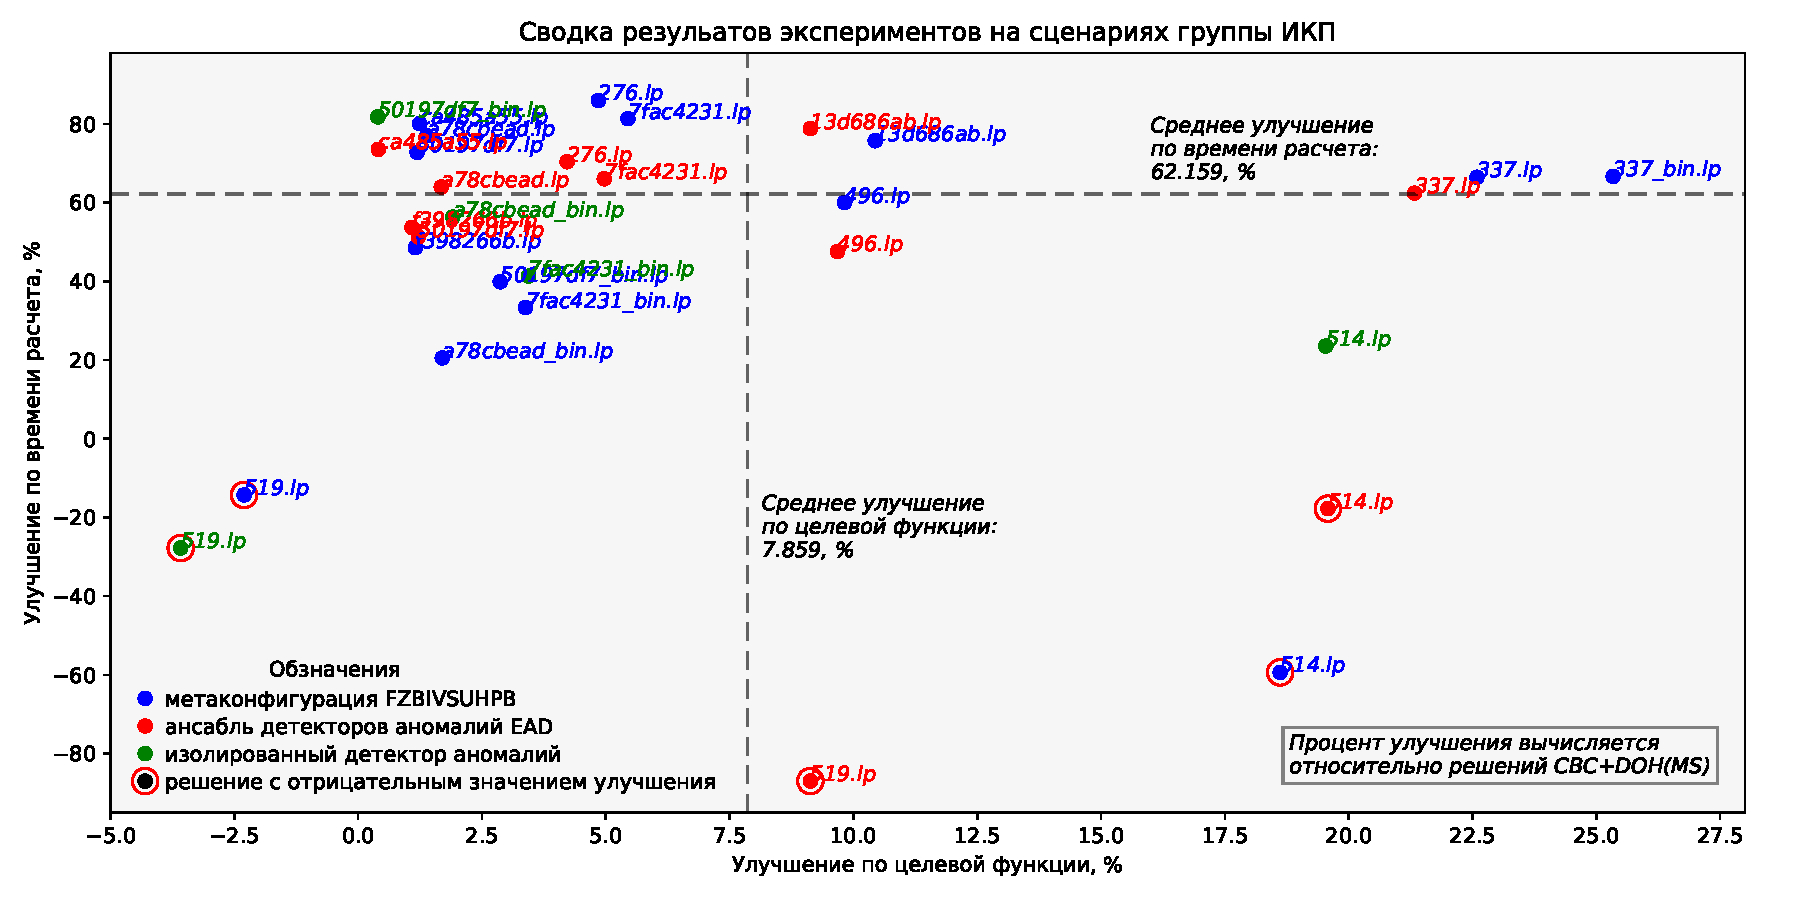
\includegraphics[scale=0.57]{figures/summary_FZB_EAD_for_IKP.pdf}
	\caption{ Сводка результатов вычислительных экспериментов на сценариях группы ИКП }\label{fig:summary_FZB_EAD_for_IKP}
\end{figure}









\section{Приемы поиска решения}

\subsection{Прием фиксации бинарно-целочисленных переменных в релаксированном решении}\label{sec:bin_int_relax_fix}

Часто фиксация целочисленных переменных\footnote{Вообще говоря, фиксировать можно не только бинарные и целочисленные переменные} в релаксированном решении приводит к приемлемому допустимому целочисленному решению, которое потом можно использовать как <<теплый старат>> или как базовое решение для других схем фиксации.
\begin{lstlisting}[
style = ironpython,
numbers = none
]
ZERO = 0.0
...
relax_sol: pd.Series = read_relax_sol(path_to_relax_sol)

model = pyscipopt.Model()
model.readProblem(path_to_lp_file)
model.readParams(path_to_set_file)

all_vars: t.List[pyscipopt.scip.Variable] = model.getVars()
bin_vars: t.List[pyscipopt.scip.Variable] = extract_vars_set_type(all_vars, BINARY)
int_vars: t.List[pyscipopt.scip.Variable] = extract_vars_set_type(all_vars, INTEGER)

all_zero_bin_vars: t.List[
	pyscipopt.scip.Variable
] = extract_from_relax_sol_zero_vars(
	relax_sol,
	sub_group_vars=bin_vars,
)
all_zero_int_vars: t.List[
	pyscipopt.scip.Variable
] = extract_from_relax_sol_zero_vars(
	relax_sol,
	sub_group_vars=int_vars,
)

for var in all_zero_bin_vars + all_zero_int_vars:
	model.fixVar(var, ZERO)

model.optimize()
...
\end{lstlisting}

\subsection{Детектирование квазинулевых бинарных и целочисленных переменных}

\subsubsection{Предложение по матрице признакового описания объекта}

Проблема <<квазинулевых>> переменных заключается в том, что некоторые бинарные и целочисленные переменные, которые принимают нулевое значение в релаксированном решении, могут принять ненулевые значения в целочисленном решении (такие переменные предлагается считать \emph{аномалиями}). Фиксация, построенная на таких <<ложных нулях>> с одной стороны обладает высокой компрессией как по переменным, так и по ограниченим (то есть значительно снижает размерность задачи), но с другой -- сильно мешает решателю.

Задача сводится к тому, чтобы научиться отличать одну нулевую бинарную или целочисленную переменную от другой. Кажется естественным для этой задачи использовать аппарат машинного обучения. Строки матрицы плана будут описывать контекст переменных и, как ожидается, помогут детектировать квазинулевые переменные с высокой полнотой и точностью.

Матрицу признакового описания объекта можно строить на переменных, которые приняли нулевое значение в релаксированном решении, найденном с помощью SCIP, и ненелувое значение в целоичесленном решении, найденном с помощью коммерческого решателя (CPLEX, Gurobi, COPT etc.). Такие переменные будем называть аномалиями и помечать единицей. Для построения задачи бинарной классификации на сбалансированном наборе данных остается только из исходной матрицы плана выбрать <<штатные>> экземпляры (помечаются 0) в количестве равном количеству аномалий.

Предлагается использовать следующие признаки:
\begin{enumerate}
	\item \verb|relax_sol| (то же, что и \verb|var_lp_sol_relax|): значения переменных в релаксированном решении,
	
	\item \verb|var_ub_global_relax|: глобальные верхние границы переменных в релаксированном решении,
	
	\item \verb|var_lp_sol_default_presolve|: значения переменных в релаксированном решении, полученном после пресолвинга с настройками по умолчанию,
	
	\item \verb|n_vars_after_presolving_default_presolve|: число переменных после пресолвинга с настройками по умолчанию.
	
	\item \verb|continuous_context_types|: число вещественных переменных, входящих в те же ограничения, что и рассматриваемая переменная,
	
	\item \verb|binary_context_types|: число бинарных переменных, входящих в те же ограничения, что и рассматриваемая переменная,
	
	\item \verb|integer_context_types|: число целочисленных переменных, входящих в те же ограничения, что и рассматриваемая переменная,
	
	\item \verb|var_mean_relax_context|: значения релаксированного решения, усредненные по переменным, входящим в те же ограничения, что и рассматриваемая переменная.
\end{enumerate}

\subsubsection{Анализ важности признаков}

Лучший набор признаков, упорядоченный по убыванию \emph{пермутационной важности}, найденной с помощью модели случайного леса (\verb|n_estimators=450|, \verb|max_features=0.25|, \verb|max_depth=8|)\footnote{На обучающем поднаборе: гармоническое среденее: 0.687, полнота: 0.6370, точность: 0.745, площадь под ROC-кривой: 0.709, на валидационном поднаборе: гармоническое среднее: 0.670, полнота: 0.628, точность: 0.720, площадь под ROC-кривой: 0.692}:
\begin{enumerate}
	\item \verb|integer_context_after_presolving|,
	
	\item \verb|var_ub_global_after_presolving|,
	
	\item \verb|relax_sol|,
	
	\item \verb|var_ub_global_relax|,
	
	\item \verb|var_context_mean_relax_after_presolving|.
\end{enumerate}

Важность признаков \emph{по Шепли}, найденная с помщью Zero-shot AutoML LIghtGBM библиотеки FLAML (\verb|boostring_type="gbdt"|, \verb|objective="binary"|, \verb|max_depth=7|) , приведена на \pic{fig:shap_imprt}.

\begin{lstlisting}[
style = ironpython,
numbers = none
]
clf_zero_shot = default.LGBMClassifier(
	boosting_type="gbdt",
	objective="binary",
	max_depth=7,  # приходится помочь; в противном случае сильно переобучается
)

clf_zero_shot.fit(X_sub_train, y_sub_train)

explainer = shap.TreeExplainer(clf_zero_shot)
shap_values_train = explainer.shap_values(X_sub_train)
shap_values_val = explainer.shap_values(X_val)

shap.summary_plot(shap_values_train[1], X_sub_train)
\end{lstlisting}

Как показывает глобальная интерпретация (\pic{fig:shap_imprt}) б\emph{о}льшие значения верхней границы после пресолвинга (признак \texttt{var\_ub\_global\_after\_presolving}) отвечают <<аномальным>> переменным. То есть другими словами чем выше верхняя граница нулевой бинарной или целочисленной переменной, тем вероятнее она примет ненулевое значение в целочисленном решении. Напротив, меньшие значения признака \texttt{integer\_context\_after\_presolving} указывают на <<аномальность>> переменной -- в среднем чем меньше целочисленных переменных в контексте рассматриваемой переменной, тем выше вероятность, что она окажется аномальной.

Ниже приводятся графики частичной зависимости признаков. График частичной зависимости признака \verb|relax_sol| (\pic{fig:part_depend_relax_sol}) показывает, что в целом низкие значения переменной в релаксированном решении отвечают <<штатным>> переменным, но есть небольшой кластер точек, которые даже если и принимают нулевое или близкое к нулю значение в релаксированном решении, все-таки оказываются аномальными. Это и есть искомые <<квазинулевые>> переменные. Здесь есть неоднозначность. Среди <<штатшных>> бинарных и целочисленных переменных чаще оказываются такие, в контексте которых мало целочисленных переменных, но есть и такие в контексте которых целочисленные переменные встречаются часто.

\begin{lstlisting}[
style = ironpython,
numbers = none	
]
shap.dependence_plot("feature_name", shap_values_val[1], X_val)
\end{lstlisting}

\begin{figure}[h]
	\centering
	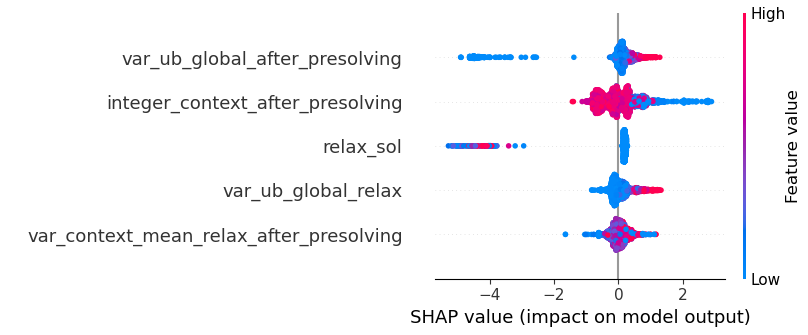
\includegraphics[scale=1.0]{figures/shap_imprt.png}
	\caption{ Важность признаков по Шепли }\label{fig:shap_imprt}
\end{figure}

\begin{figure}[h]
	\centering
	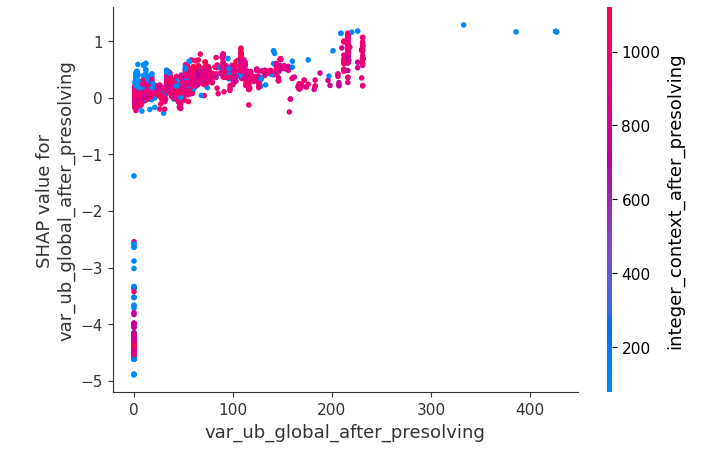
\includegraphics[scale=0.90]{figures/part_depend_var_ub_global.png}
	\caption{ График частичной зависимости признака \texttt{var\_ub\_global\_after\_presolving} \\от признака \texttt{integer\_context\_after\_presolving}  }\label{fig:part_depend_var_ub_global}
\end{figure}

\begin{figure}[h]
	\centering
	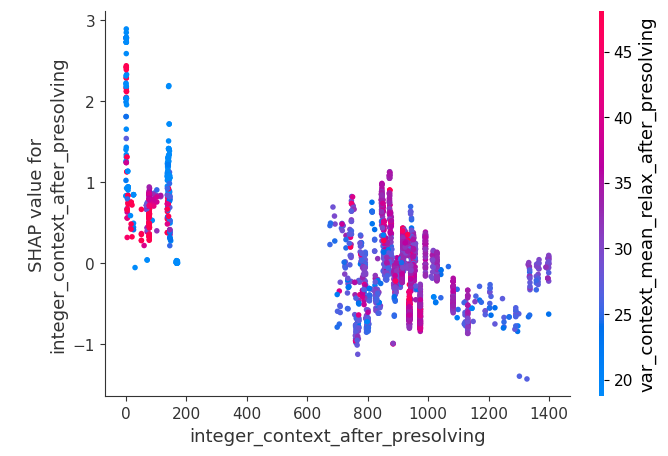
\includegraphics[scale=0.90]{figures/part_depend_integer_context.png}
	\caption{ График частичной зависимости признака \texttt{integer\_context\_after\_presolving} \\от признака \texttt{var\_context\_mean\_relax\_after\_presolving} }\label{fig:part_depend_integer_context}
\end{figure}

\begin{figure}[h]
	\centering
	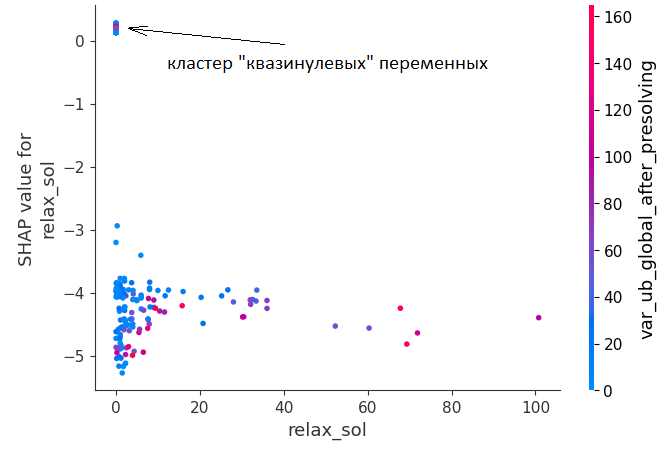
\includegraphics[scale=0.90]{figures/part_depend_relax_sol.png}
	\caption{ График частичной зависимости признака \texttt{relax\_sol} \\от признака \texttt{var\_ub\_global\_after\_presolving} }\label{fig:part_depend_relax_sol}
\end{figure}

Пострим локальную интерпретацию на экземплярах. Для проверки вычислим значения Шепли с помощью встроенных средств LightGBM и с помощью библиотеки SHAP. Важно помнить, что в отличие от библиотеки SHAP, метод \verb|predict| с флагом \verb|predict_contib=True| библиотеки LightGBM возвращает матрицу размером $ n\_samples \times (n\_features + 1) $, а не $ n\_samples \times n\_features $. Последний столбец в матрице это ожидаемое значение (expected value\footnote{Оно же  на графиках локальной интерпретации библиотеки SHAP обозначается как <<base value>>}) \url{https://lightgbm.readthedocs.io/en/latest/pythonapi/lightgbm.LGBMClassifier.html#lightgbm.LGBMClassifier}.
\begin{lstlisting}[
style = ironpython,
numbers = none
]
clf_zero_shot.predict(
    X_val,
    pred_contrib=True
)[:, :-1].sum(axis=1)[SAMPLE_IDX]  # -0.49065584326131984

shap_values_val[1][SAMPLE_IDX, :].sum()  # -0.49065584326131984
\end{lstlisting}

И, наконец, строим локальную интерпретацию для первого экземпляра валидационного поднабора (см. \pic{fig:local_interpr_shap})
\begin{lstlisting}[
style = ironpython,
numbers = none
]
SAMPLE_IDX = 0

shap.force_plot(
    explainer.expected_value[1],
    shap_values_val[1][SAMPLE_IDX, :],
    X_val.iloc[SAMPLE_IDX, :]
)
\end{lstlisting}

\begin{figure}[h]
	\centering
	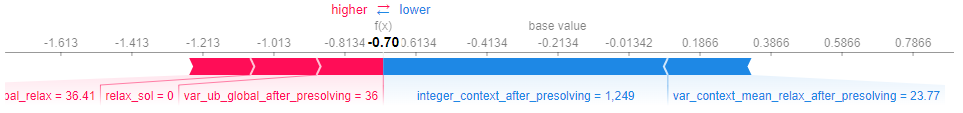
\includegraphics[scale=0.90]{figures/local_interpr_shap.png}
	\caption{ Локальная интерпретация для первого экземпляра валидационного поднабора }\label{fig:local_interpr_shap}
\end{figure}



\subsection{Прием подавления подгруппы первичных эвристик низкой эффективности}\label{sec:suh}

В некоторых случаях отдельные первичные эвристики могут оказаться не способными справится со своей задачей, не оказывая никакого влияния на процедуру поиска решения, и все же потреблять предоставленные ресурсы.

Такие эвристики -- условимся их называть первичными эвристиками низкой эффективности (ПЭНЭ) -- можно выявить путем анализа статистической сводки \verb|stat|-файла в разделе Primal Heuristics
\begin{lstlisting}[
title = {\sffamily Фрагмент файла статистической сводки 337\_bin\_default.stat},
style = bash,
numbers = none
]
...
Primal Heuristics  :   ExecTime  SetupTime      Calls      Found       Best
  LP solutions     :       0.00          -          -          0          0
	relax solutions  :       0.00          -          -          0          0
	pseudo solutions :       0.00          -          -          0          0
	...
	conflictdiving   :       0.00       0.00          0          0          0
	crossover        :       0.00       0.00          0          0          0
	dins             :       0.00       0.00          0          0          0
	distributiondivin:       0.00       0.00          0          0          0
	dualval          :       0.00       0.00          0          0          0
	farkasdiving     :    2032.89       0.00          1          0          0  # <- NB
	feaspump         :     882.12       0.00          1          0          0  # <- NB
	fixandinfer      :       0.00       0.00          0          0          0
	...
	intdiving        :       0.00       0.00          0          0          0
	intshifting      :      52.99       0.00          1          1          1
	...
\end{lstlisting}

В данном случае ПЭНЭ являются \texttt{farkasdiving} и \texttt{feaspump}. Чтобы подавить эти эвристики при следующем запуске \texttt{SCIP}, достаточно включить следующие строки в конфигурационный файл \texttt{scip.set}\footnote{При запуске интерактивной сесии через утилиту командной строки \texttt{scip}, решатель ищет этот файл в текущей директории и, если находит, автоматически вычитывает. При работе через PySCIPOpt требуется явно передавать путь до файла методу модели \texttt{readParams()}}
\begin{lstlisting}[
title = {\sffamily scip.set},
style = bash,
numbers = none
]
...
heuristics/farkasdiving/freq = -1
heuristics/feaspump/freq = -1
...
\end{lstlisting}

Доступ к статистической сводке можно получить либо в сессии \texttt{SCIP}, либо через одну из оберток над решателем (например, с помощью PySCIPOpt)
\begin{lstlisting}[
title = {\sffamily Фрагмент сессии scip. Получение статистической сводки},
style = bash,
numbers = none
]
...
SCIP> read file.lp
SCIP> opt
SCIP> display stat
\end{lstlisting}

\begin{lstlisting}[
title = {\sffamily Получение статистической сводки через обертку PySCIPOpt},
style = ironpython,
numbers = none
]
import pyscipopt

model = pyscipopt.Model()
model.readProblem("...")
model.readParams("...")
model.optimize()

model.printStatistics()
\end{lstlisting}





\subsection{Прием подбора порога бинаризации для бинарных переменных в релаксированном решении}\label{sec:find_bin_thresh}

Условимся \emph{фиксацией} называть стратегию инициализации подгруппы переменных $ x_k $ (вещественных, бинарных или целочисленных), значения которых задаются на основе каких-либо эврестических соображений, например, касающихся специальных свойств матрицы ограничений, и способных в результате привести к такой постановке задачи, которую, используя механизмы первичных эвристик, сепараторов, пропагаторов и пр. можно развить в \emph{допустимое целочисленное решение}.

Базовая идея построения \emph{фиксации на бинарных переменных} заключается в том, чтобы значения бинарных переменных в релаксированном решении\footnote{Верхний левый индекс <<$ r $>> указывает на релаксированное значение, а верхний правый <<$ (b) $>> -- на то, что речь идет о бинарной переменной} $ {\{{}^rx^{(b)}_k\}}_{k=1, \ldots} $ интерпретировать как \emph{степень уверенности} решателя в том, что рассматриваемую бинарную переменную можно выставить в единицу.

Если значение $ k $-ой бинарной переменной $ {}^rx_k^{(b)}$ превосходит некоторый \emph{порог}~$ \theta $, то переменная выставляется в единицу, в противном случае -- в ноль. Порог подбирается итерационно, начиная с некоторого нижнего значения $ \theta_l $ (по умолчанию $ \theta_l = 0 $), увеличивая текущее значение порога на величину шага $ \Delta \theta $ и заканчивая верхним значением порога $ \theta_u $ (по умолчанию $ \theta_u = 1 $).

Для практических целей достаточно остановится на наименьшем значении порога $ \theta $, который отвечает такой фиксации, которую решатель SCIP не отклоняет как неспособную привести к допустимому целочисленному решению.
\begin{lstlisting}[
title = {\sffamily Фрагмент лога решателя SCIP для случая фиксации, которую невозможно развить\\ в допустимое целочисленное решение},
style = bash,
numbers = none	
]
...
SCIP Status        : problem is solved [infeasible]
Solving Time (sec) : 3.00
Solving Nodes      : 0
Primal Bound       : +1.00000000000000e+20 (0 solutions)
Dual Bound         : +1.00000000000000e+20
Gap                : 0.00 %
original problem has 740251 variables (2666 bin, 147789 int, 0 impl, 589796 cont) and 545350 constraints
...
\end{lstlisting}

После того как порог $ \theta $ подобран, бинарные переменные разбиваются на две подгруппы: подгруппу бинарных переменных, выставленных в ноль $ \{x_k^{(b_0)}\} $, и подгруппу бинарных переменных, выставленных в единицу $ \{ x_k^{(b_1)} \} $. Долю бинарных переменных, выставленных в ноль обозначим через~$ \delta_{b_0} $, долю бинарных переменных, выставленных в единицу -- через $ \delta_{b_1} $, а целевую функцию, найденную при заданных долях -- через $ f_{\theta}(\delta_{b_0}, \delta_{b_1}) $.

В результате получаем исследовательский инструмент, который дает возможность управлять решением через подбор долей $ \delta_{b_0} $ и $ \delta_{b_1} $ при найденном пороге $ \theta $. Часто оказывается эффективным прием управления решением через подбор доли нулевых бинарных переменных $ \delta_{b_0} $.

Целевая функция, вычисленная при единичной доле нулевых бинарных переменных $ f_{\theta}(\delta_{b_0}=1) $, как правило, значительно уступает целевой функции релаксированного решения $ f_r $. Но тем неменее это решение может быть улучшено, сокращением доли $ \delta_{b_0} $ (см.~\pic{fig:a78cbeadfracbinzeros} и \pic{fig:337fracbinzeros}).

\begin{figure}[!h]
	\centering
	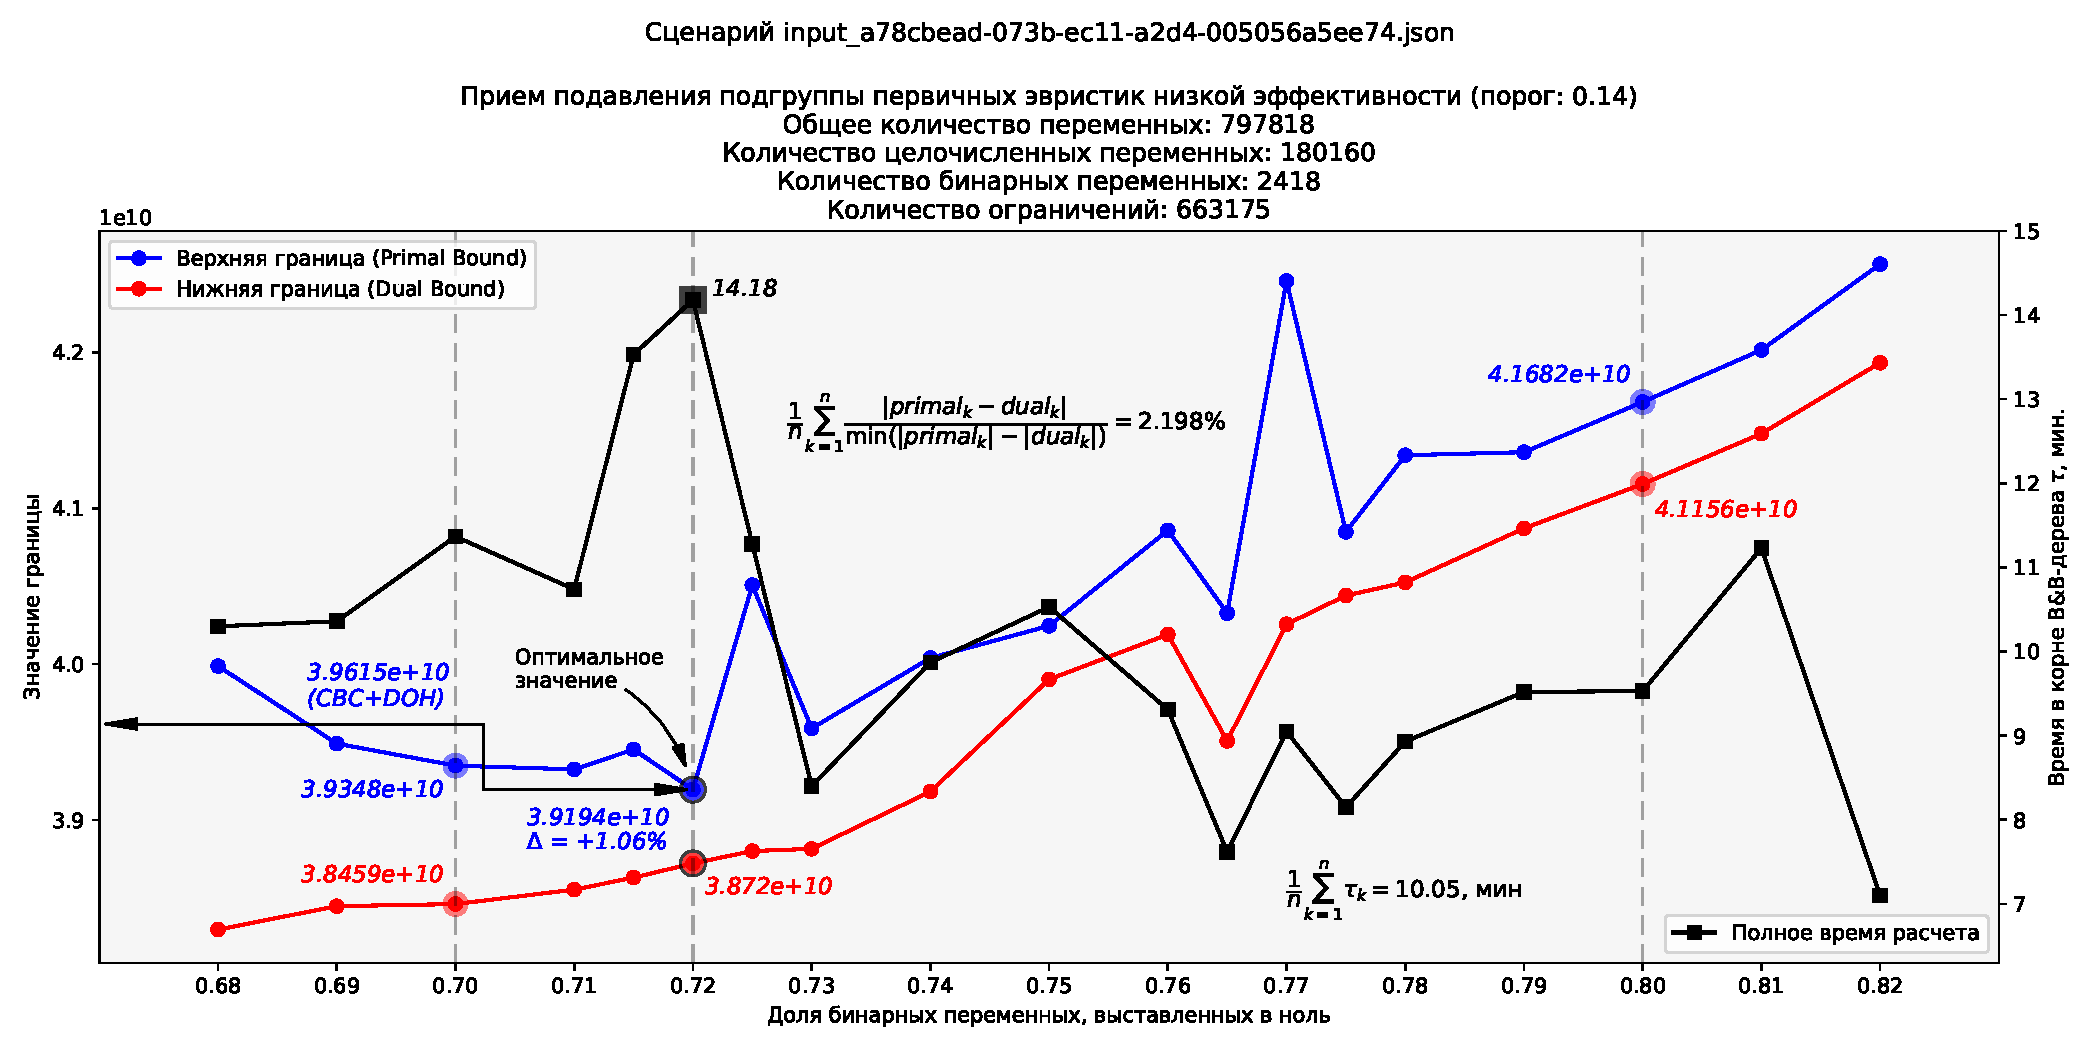
\includegraphics[scale=0.45]{figures/a78cbead_frac_bin_zeros.pdf}
	\caption{ Зависимость верхней границы решения от доли бинарных переменных, \\выставленных в ноль. Сценарий \texttt{a78cbead} }\label{fig:a78cbeadfracbinzeros}
\end{figure}

\begin{figure}[!h]
	\centering
	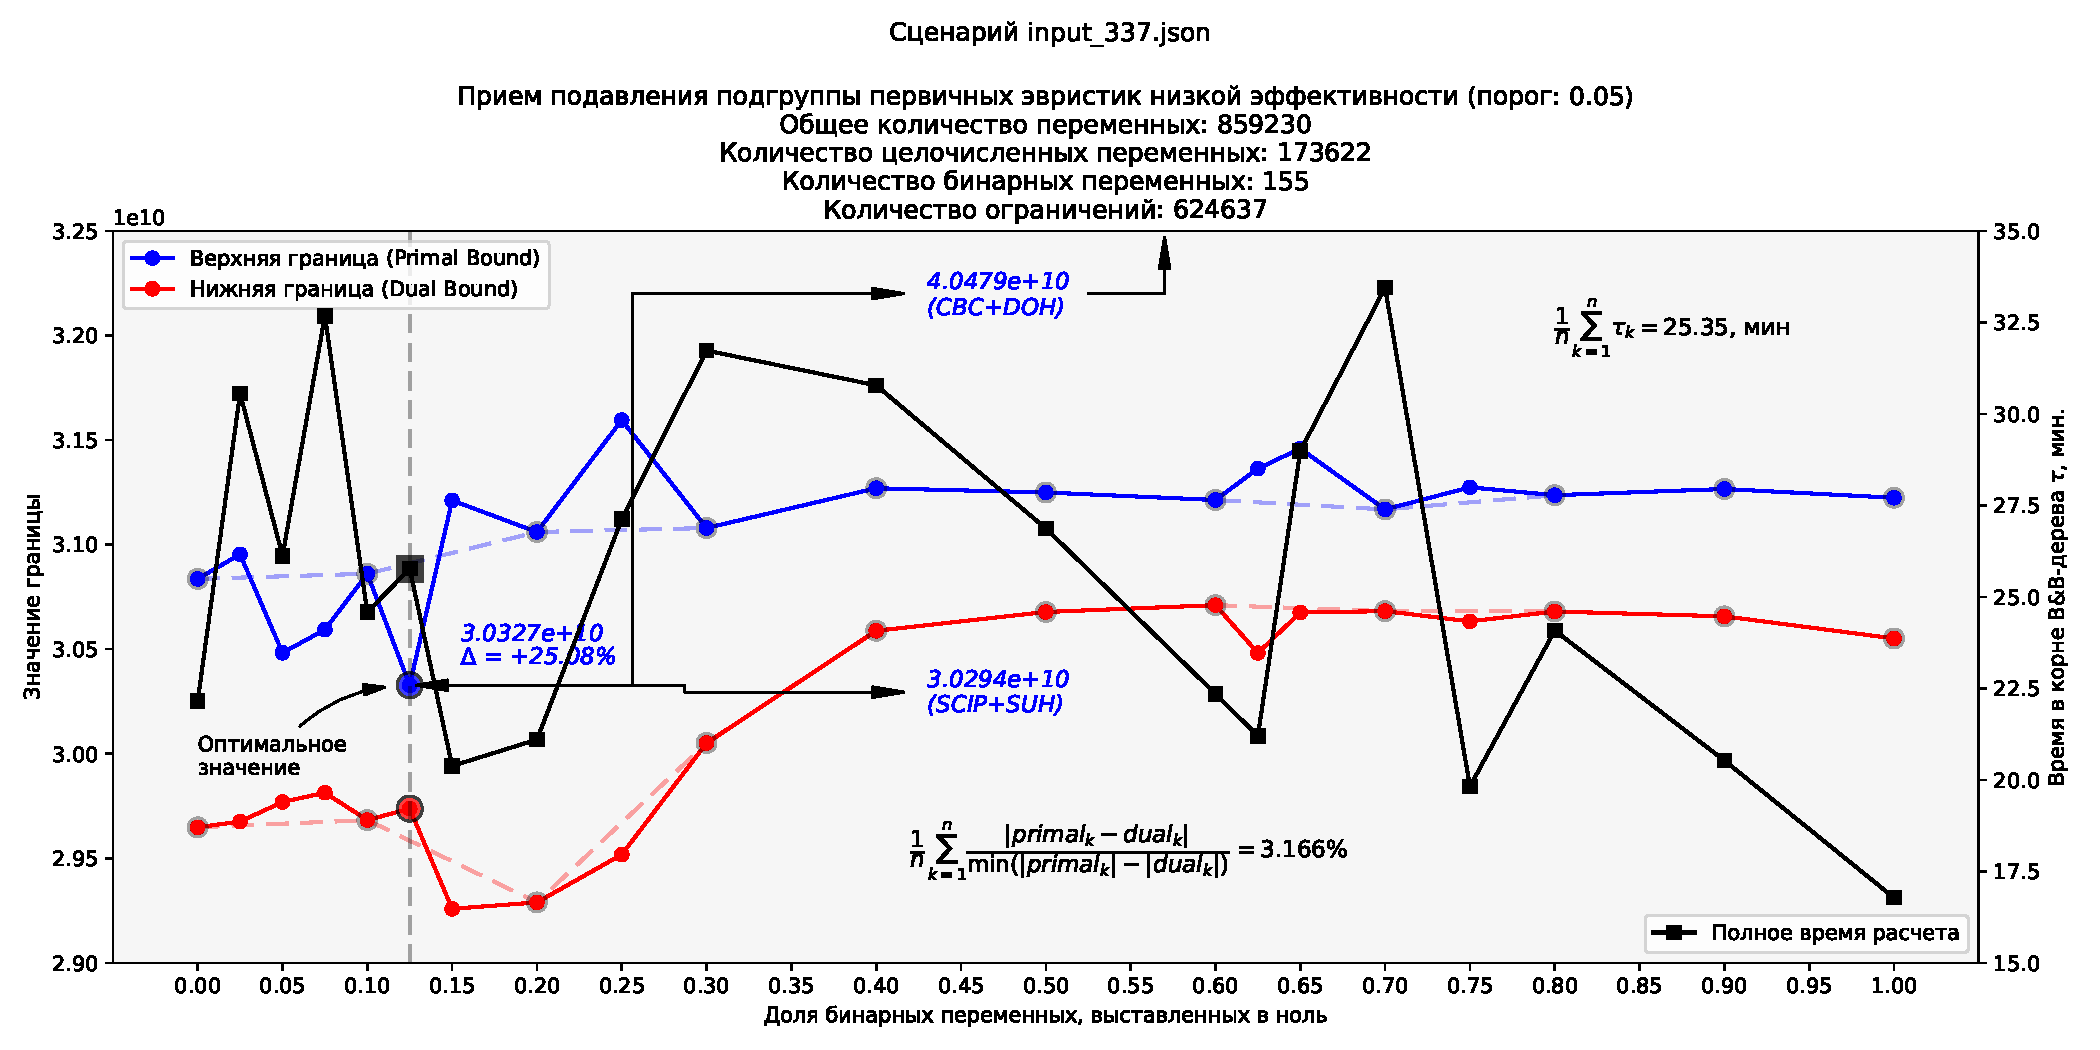
\includegraphics[scale=0.45]{figures/337_frac_bin_zeros.pdf}
	\caption{ Зависимость верхней границы решения от доли бинарных переменных, \\выставленных в ноль. Сценарий \texttt{337} }\label{fig:337fracbinzeros}
\end{figure}

Как видно из графиков, на кривой изменения верхней границы решения существует точка с наименьшим значением целевой функции $ f_{\theta}(\delta_{b_0}) $ допустимого целочисленного решения. Эта точка и будет <<оптимальной>> для рассматриваемого сценария.

\section{Методы машинного обучения в задачах комбинаторной оптимизации}

\subsection{Постановка задачи}

Цель: Разработать процедуру построения частично-заданного решения на фиксациях для сценариев с матрицей ограничений произольной структуры.

Вход: произвольная матрица ограничений\footnote{Предполагается, что матрица ограничений имеет низкую меру обусловленности}.

Выход: набор бинарных и целочисленных переменных, фиксация которых в ноль с высокой вероятностью приведет к допустимому целочисленному решению.

База: частично-заданное решение, построенное на фиксациях нулевых бинарных и целочисленных переменных в релаксированном решении.

\subsection{Концепт матрицы признакового описания бинарных и целочисленных переменных}

В качестве признаков бинарно-целочисленных переменных предлагается использовать:
\begin{enumerate}
	\item {\color{deepgreen} \itshape важный признак} Значение переменной $ x_i $ в <<усредненном>> релаксированном решении\footnote{Задача линейного программирования в релаксированной постановке решается с использованием различных методов (двойственный симплекс-метод, метод внутренней точки и т.д.), а затем полученные решения усредняются},
	
	\item Модифицированную Z-оценку на <<усредненном>> релаксированном решении,
	
	\item {\color{red} \itshape бесполезный признак} Дробную часть значения переменной $ x_i $ в <<усредненном>> релаксированном решении,
	
	\item {\color{deepgreen} \itshape важный признак} Пороги бинаризации на <<усредненном>> релаксированном решении (каждый порог это отдельный принак),
	
	\item {\color{deepgreen} \itshape важный признак} Число ограничений $ n_i $, в которые входит рассматриваемая переменная $ x_i $,
	
	\item {\color{deepgreen} \itshape важный признак} Число положительных $ n_i^{+} $ и отрицательных $ n_i^{-} $ коэффициентов в ограничениях, ассоциированных с рассматриваемой переменной $ x_i $,
	
	\item Булев маркер удаления переменной $ x_i $ после шага снижения размерности задачи,
	
	\item {\color{deepgreen} \itshape важный признак} Коэффицент $ c_i $ при переменной $ x_i $ в целевой функции $ \mathbf{c}^T \mathbf{x} $,
	
	\item {\color{red} \itshape бесполезный признак} Вероятность\footnote{Идея построения признака основана на способе вычисления вероятности единичного выхода нейрона в машинах Больцмана \cite[\strbook{653}]{geron:ml-2018}} того, что $ i $-ая бинарная или целочисленная переменная $ x_i $ будет выставлена в~1 (индекс <<$ {-i} $>> означает без учета $ i $-ой переменной)
	\begin{align*}
		\mathbf{P}(x_i = 1) = \sigma \bigg( \dfrac{1}{t} \, (\mathbf{c}^T \mathbf{x})_{-i} \bigg),
	\end{align*}
	где $ \sigma $ -- логистический сигмоид, $ t $ -- <<температура>> (чем выше температура, тем случайнее выход), $ \mathbf{c} $ -- вектор коэффициентов целевой функции, $ \mathbf{x} $ -- вектор значений переменных в релаксированном решении.
	
	\item Важность $ x_i $ переменной с точки зрения пресолверов.
\end{enumerate}

\subsection{Стратегии решения задачи}

\subsubsection{Стратегия №1. Обнаружение аномалий}\label{sec:obj_detect}

%С помощью техник t-SNE и LLE найти низкоразмерное представление бинарно-целочисленных переменных. Оценить пермутационную важность признаков и важность признаков по Шепли.
%
%Оценить меру похожести \emph{релаксированного решения} $ {}^r\{x_k\}_{k=1}^M $ и \emph{допустимого целочисленного решения} $ {}^f\{x_k\}_{k=1}^M $, например, с помощью \emph{коэффициента Отиаи}\footnote{\url{https://en.wikipedia.org/wiki/Cosine_similarity}}
%\begin{align*}
%	K = \bigg[ \dfrac{ \# {}^r\{x_k\}\bigcap {}^f\{x_k\} }{M} \bigg]^2, \quad K \in [0, 1],
%\end{align*}
%где $ {}^r\{x_k\} $ -- набор значений переменных в релаксированном решении; $ {}^f\{x_k\} $ -- набор значений переменных в допустимом решении; $ \# x \bigcap y $ -- количество переменных на пересечении решений $ x $ и $ y $; $ M $ -- количество переменных в сценарии.
%
%Если релаксированное решение и допустимое целочисленное не пересекаются, то есть не имеют переменных с одним и тем же значением, то очевидно коэффициент Отиаи равен нулю. Если же решения пересекаются по всем переменным, то коэффициент становится равным единице. 

Задачу построения частично-заданного решения на фиксациях предлагается свести к задаче обнаружения аномалий в данных. Бинарные и целочисленные переменные, которые {как ожидается} примут \emph{нулевые значения} в допустимом целочисленном решении будем считать <<\underline{штатным}>> \underline{режимом}, а бинарные и целочисленные переменные, которые {как ожидается} примут \emph{ненулевые значения} в допустимом целочисленном решении -- \underline{аномалиями}. Такие <<аномальные>> экзмепляры остаются без рекомендуемого значения для фиксации, а оставшиеся нулевые <<штатные>> бинарные и целочисленные переменные фиксируются в ноль и на этом процедура построения частично-заданного решения считается завершенной.

Для повышения надежности прогноза предлагается использовать ансамбль детекторов аномалий. Решение о фиксации бинарной или целочисленной переменной в ноль принимается на основании большинства голосов ансамбля детекторов.

Набор данных представляет собой неупорядоченную коллекцию матриц признакового описания, ассоциированных с соответствующими lp/mps-файлами математической постановки задачи (условимся называть их \emph{сценариями}).



Ансамбль детекторов аномалий обучается по роторной схеме:
\begin{itemize}
	\item На $ i $-ой итерации все \emph{матрицы признакового описания} (всего в наборе $ S $ матриц/сценариев) кроме $ i $-ой матрицы используются для обучения детекторов, а на $ i $-ой матрице признакового описания строится прогноз аномальных экземпляров, которые помечаются как <<-1>>. В результате получается коллекция бинарных и целочисленных переменных, помеченных либо как <<0>>, либо как <<-1>>. Построенное решение сравнивается с допустимым целочисленным решением с помощью различных метрик качества (параметрическое гармоническое среднее, каппа Коэна, коэффициент корреляции Метьюса и т.д.). Вычисленные для $ i $-ой матрицы метрики качества и построенное частично-заданное решение на фиксациях сохраняются в директории результатов,
	
	\item Затем описанный шаг повторяется для оставшихся матриц признакового описания объекта.
\end{itemize}

По окончании процедуры для каждого сценария:
\begin{itemize}
	\item будут вычислены метрики качества,
	
	\item будет построенно частично-заданное решение на фиксациях,
\end{itemize}

Полученные частично-заданные решения на фиксациях подаются на вход решателю SCIP. Если SCIP удалось найти решение, обозначаемое как $ s_{\text{ML}} $, то оно сравнивается с решением $ s_{\text{FZB}} $, полученным с помощью метаконфигурации FZBIVSUHPB (см. подраздел~\ref{sec:ikp_bins}), по времени работы и по значению верхней гранцы решения.

\remark{
Как правило, в задачах обнаружения аномалий не выполняют подбор гиперпараметров детектора, но в данном случае кажется полезным изучить поведение детектора хотя бы в зависимости от параметра контаминации. Дело в том, что на практике эффективность детектора может существенно изменяться в зависимости от значений управляющих параметров
}

На всех сценариях группы ИКП (см. раздел~\ref{sec:ikp}) обнаруживается серьезный дисбаланс экземпляров положительного (<<аномалии>>, ненулевые значения переменных) и отрицательного (<<штатные>> экземпляры, нулевые значения переменных) классов. Ожидается, что эффективность модели машинного обучения главным образом будет зависеть от способности модели выявлять аномальные экземплеры.

Действительно, \emph{ошибка первого рода} (ложное срабатывание, т.е. когда отрицательный <<штатный>> экземпляр принимается за <<аномальный>> положительный) приводит к тому, что нулевая переменная \emph{не будет} зафиксирована в ноль в частично-заданном решении, что с высокой вероятностью снизит производительность решателя SCIP.

Тогда как \emph{ошибка второго рода} (пропуск объекта, т.е. когда <<аномальный>> положительный экземпляр принимается за <<штатный>> отрицательный) приводит к тому, что ненулевая переменная в частично-заданном решении будет зафиксирована в ноль. Это сделает частично-заданное решение не способным развиться в допустимое целочисленное, что значительно хуже.

Таким образом, кажется разумным сосредоточить усилия на том, чтобы минимизировать {ошибку второго рода}, и в результате свести к минимуму число пропусков аномалий.

Проще всего оценить качество модели с учетом б\emph{о}льшего влияния ошибок второго рода с помощью \href{https://scikit-learn.org/stable/modules/model_evaluation.html#precision-recall-f-measure-metrics}{$ F_{\beta} $-меры} при значениях параметра $ \beta > 1 $
\begin{align*}
	F_{\beta} = (1 + \beta^2) \, \dfrac{\text{precision} \cdot \text{recall}}{\beta^2\, \text{precision} + \text{recall}},
\end{align*}
где $ \text{precision} $ -- точность, $ \text{recall} $ -- полнота.

\remark{
Провести анализ приема подбора порога бинаризации. И проработать схему подбора гиперпараметров детекторов
}

\paragraph{Анализ производительности методов обнаружения аномалий} 

Рекомендуемые значения некотрых гиперпараметров для детекторов некоторых семейств звучат следующим образом \cite{soenen:effect-hyper-param-tuning:2021}:
\begin{itemize}
	\item для KNN (k Nearest Neighbors\footnote{Расстояние от $ k $-ого ближайшего соседа рассматривается как мера аномальности экземпляра}) и LOF (Local Outlier Factor): $ k = \max (10; 0.03 \, |D|) $, где $ |D| $ - число экземпляров в наборе данных,
	
	\item для HBOS (Histogram-based Outlier Score): \texttt{n\_bins} $ = \sqrt{|D|} $,
	
	\item для IForest (Isolation Forest): число деревьев \texttt{n\_estimators=100 } и число экземпляров на дерево \texttt{max\_samples=256},
	
	\item для CBLOF (Clustering-Based Local Outlier Factor): $ \alpha = 0.90 $, $ \beta = 5 $ и $ k = 10 $,
	
	\item для OCSVM (One-Class Support Vector Machines): ядро RFB($ \nu = 0.5, \gamma = 1/m $), где $ m $ - число признаков в наборе данных $ D $.
\end{itemize}
\vspace*{2mm}

Перечисленные ниже детекторы показали крайне низкую производительность на сценариях группы ИКП: 
\begin{itemize}
	\item KNN,
	
	\item Feature Bagging,
	
	\item ABOD (Angle-Based Outlier Detection using approximation)/FastABOD,
	
	\item LOCI (Fast outlier detection using the local correlation integral),
	
	\item CBLOF (Clustering-Based Local Outlier Factor): достаточно быстрый, но результаты отвратительные (очень низкие значения ключевых метрик качества),
	
	\item XGBOOD\footnote{Требует разметки} (Extreme Boosting Based Outlier Detection): безумно медленный\footnote{В \url{https://github.com/yzhao062/pyod/issues/152} рекомендуется использовать SUOD},
	
	\item R-Graph (Outlier detection by R-graph).
\end{itemize}
\vspace*{2mm}

Главный детектор аномалий предлагается строить с помощью агрегатора SUOD\footnote{\url{https://www.andrew.cmu.edu/user/yuezhao2/papers/21-mlsys-suod.pdf}} (Accelerating Large-scale Unsupervised Heterogeneous Outlier Detection) на следующих базовых детекторах:
\begin{itemize}
	\item ECOD (Unsupervised Outlier Detection Using Empirical Cumulative Distribution Functions),
	
	\item COPOD (Copula-Based Outlier Detection),
	
	\item IForest (Isolation Forest),
	
	\item HBOS (Histogram-based Outlier Score).
\end{itemize}



\subsubsection{Стратегия №2. Бинарная классификация со слабо выраженным миноритарным классом} Задачу построения частично-заданного решения на фиксациях предлагатеся свести к задаче бинарной классификации со слабо выраженным миноритарным классом (данные с сильным дисбалансом).

\emph{Раздел в разработке ...}

\subsection{Трансфер выявленного паттерна. Сценарии группы СОП}

Условимся \emph{трансфером выявленного паттерна} (или просто \emph{трансфером паттерна}) называть являение, состоящее в том, что модель, обученная на сценариях одной группы (сценарии обучающего поднабора), оказывается способной строить корректные прогнозы на сценариях другой группы (сценарии тестового поднабора), обладающих четкими дискриминирующими атрибутами (структурные особенности матрицы ограничений и пр.), которые позволяют с высокой степенью уверенности отделять сценарии обучающего поднабора от сценариев тестового поднабора.

Другими словами, в отличие от классической постановки машинного обучения -- в которой экземпляры обучающего и тестового поднаборов данных должны быть похожи друг на друга -- в данном случае модель машинного обучения предлагается обучать и тестировать на сценариях, которые значимо отличаются друг от друга по каким-то ключевым аттрибутам.

\subsubsection{Сценарий \texttt{tmpfvpqodxw.lp} без бинарных переменных}

Исследование вопроса о трансфере паттерна начнем с рассмотрения простого сценария  группы СОП \texttt{tmpfvpqodxw.lp} \url{https://disk.yandex.ru/d/K7bvClpltotqlg}, а обучать модель машинного обучения будем в соответствие со стратегией №1 (\str{sec:obj_detect}).

В случае сценария \texttt{tmpfvpqodxw.lp} для простоты можно ограничиться рассмотрением только детектора HBOS (без агрегации прогнозов других детекторов с помощью обертки SUOD) и обучать его на сценарии группы ИКП \texttt{f398266b\_bin.lp} (см. раздел~\ref{sec:f398266b_bin}).

Для того чтобы использовать не ансамбль детекторов аномалий, а лишь какой-то конкретный детектор, достаточно в конфигурационном файле \texttt{main\_config.yaml} передать полю \texttt{use} детектора значение \texttt{False}
\begin{lstlisting}[
title = {\sffamily main\_config.yaml. Использовать только детектор HBOS},
style = bash,
numbers = none
]
...
detector_config:
	# Строит ансамбль детекторов аномалий
	SUOD:  # Scalable Unsupervised Outlier Detection https://www.andrew.cmu.edu/user/yuezhao2/papers/21-mlsys-suod.pdf
		use: !!bool False  # <--- NB
		# Допустимые значения 'combination': average, maximization
		combination: !!str average  # стратегия агрегации прогнозов ансамбля детектеров
		contamination: !!float 0.10  # доля выбросов в наборе данных; принимает значения из диапазона (0.0; 0.5)
		n_jobs: -1  # число параллельно выполняемых задач
		verbose: !!bool True  # флаг подробного вывода информации о построении модели
	# Перечень детекторов для SUOD-ансамбля. Если SUOD.use=True, то перечисленные ниже детекторы, у которых
	# атрибут DETECTOR.use=True, будут добавлены в список SUOD().base_estimators.
	# Если SUOD.use=False, то поиск аномалий будет выполняться с помощью одного из приведенных ниже детекторов,
	# у которого атрибут DETECTOR.use=True
	COPOD:  # Copula Based Outlier Detector
		use: !!bool False  # <--- NB
		contamination: !!float 0.10  # доля выбросов в наборе данных; принимает значения из диапазона (0.0; 0.5)
		n_jobs: -1  # число параллельно выполняемых задач
	ECOD:  # Unsupervised Outlier Detection Using Empirical Cumulative Distribution Functions
		use: !!bool False  # <--- NB
		contamination: !!float 0.10  # доля выбросов в наборе данных; принимает значения из диапазона (0.0; 0.5)
		n_jobs: -1  # число параллельно выполняемых задач
	IForest:  # Wrapper of scikit-learn Isolation Forest with more functionalities
		use: !!bool False  # <--- NB
		n_estimators: !!int 250  # число деревьев принятния решений в лесе
		contamination: !!float 0.10  # доля выбросов в наборе данных; принимает значения из диапазона (0.0; 0.5)
		n_jobs: -1  # число параллельно выполняемых задач
	HBOS:  # Histogram-based outlier detection
		use: !!bool True  # <--- NB
		n_bins: !!int 10  # число бинов для построения гистограммы
		alpha: !!float 0.05  # параметр регуляризации
		contamination: !!float 0.10  # доля выбросов в наборе данных; принимает значения из диапазона (0.0; 0.5)
\end{lstlisting}

Приведенный на рис.~\ref{fig:summary_tmpfvpqodxw} график показывает, что
\begin{itemize}
	\item настройки решателя SCIP, ответственные за выбор переменных при \emph{ветвлении}\footnote{Параметр \texttt{branching/preferbinary}} и \emph{разрешении конфликтов}\footnote{Параметр \texttt{conflict/preferbinar}}, а также прием подавления подгруппы первичных эвристик низкой эффективности помогают снизить временные издержки при незначительном ухудшении целевой функции (зеленая кривая) относительно решения, полученного с помощью решателя SCIP с настройками по умолчанию (красная кривая),
	
	\item дополнительное снижение временных затрат можно получить подбором гиперпараметров детектора\footnote{В данном случае подбирался только гиперпараметр контаменации} (синяя кривая).
\end{itemize}

\begin{figure}[!h]
	\centering
	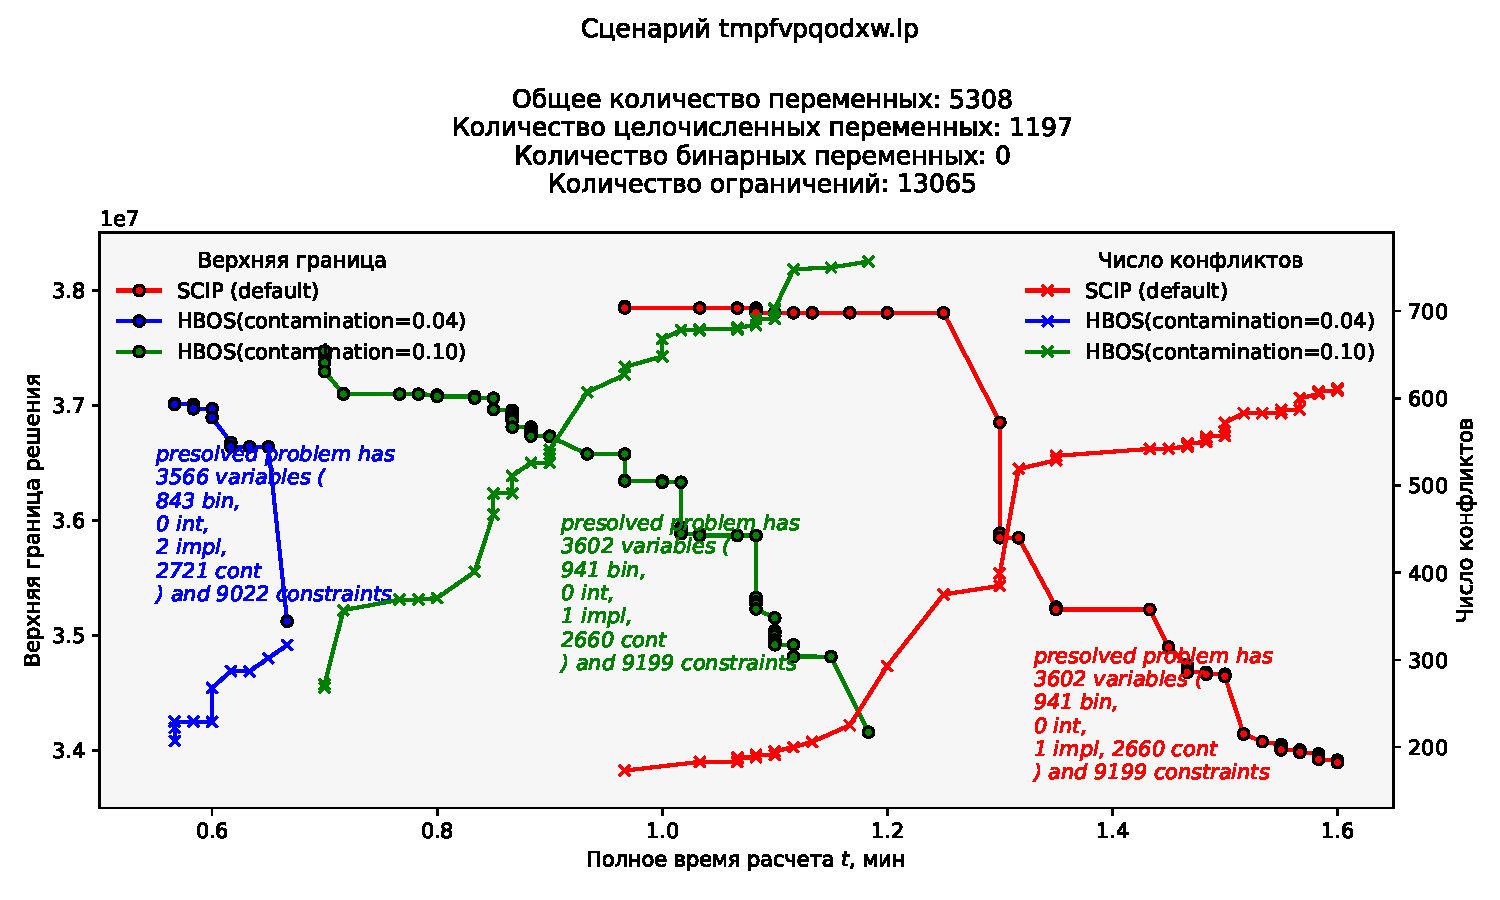
\includegraphics[scale=0.7]{figures/tmpfvpqodxw_edo.pdf}
	\caption{ Сводка результатов вычислительных экспериментов \\на сценарии группы СОП \texttt{tmpfvpqodxw.lp} }\label{fig:summary_tmpfvpqodxw}
\end{figure}

Детектору аномалий HBOS с подбором параметра контаменации (\texttt{contamination=0.04})\footnote{В библиотеке PyOD все детекторы аномалий имеют контаминацию уровня 0.10} удалось снизить количество бинарных переменных -- на 98, ограничений -- на 177, а  временные издержки снизились в 2.38 раза.


\subsubsection{Синтетический сценарий \texttt{1664182546\_82382.lp} с бинарными переменными}

\textbf{Статистика}\footnote{В скобках указана размерность задачи после шага пресолвинга с фиксацией, полученной с помощью ансамбля детекторов аномалий без подбора гиперпараметров детекторов}\vspace*{1mm}

Общее количество переменных: 5100 (4123)

Количество целочисленных переменных: 0 (0)

Количество бинарных переменных: 1768 (1132)

Количество ограничений: 11193 (10461)

lp-файл: \url{https://disk.yandex.ru/d/FuEBWt4zvFIsEA}

Блок подавления подгруппы первичных эвристик низкой эффективности конфигурационного файла SCIP
\begin{lstlisting}[
title = {\sffamily Фрагмент файла scip.set. Сценарий 1664182546\_82382.lp},
style = bash,
numbers = none
]
...
heuristics/adaptivediving/freq = -1
heuristics/fracdiving/freq = -1
heuristics/linesearchdiving/freq = -1
heuristics/objpscostdiving/freq = -1
heuristics/pscostdiving/freq = -1
heuristics/rootsoldiving/freq = -1
heuristics/veclendiving/freq = -1
\end{lstlisting}

На рис.~\ref{fig:1664182546_82382} приведены результаты сравнительного анализа запусков i) решателя SCIP с настройками по умолчанию, ii) решателя SCIP на частично-заданном решении, полученном с помощью ансамбля детекторов аномалий, и iii) решателя SCIP на фиксации, подговтоленной с помощью изолированного детектора HBOS.

Как видно из рисунка, решатель SCIP с настройками по умолчанию (синяя кривая) первое допустимое целочисленное решение с адекватным зазором находит гораздо позже схемы на частично-заданном решении, полученном с помощью ансамбля детекторов (красная кривая). Однако, спустя некоторое время схема с настройками по умолчанию быстрее выходит на конкурентное значение целевой функции (41389.75 против 41557.30).

Схема с подбором гиперпараметра контаменации изолированного детектора HBOS, несмотря на то, что размерность задачи снижается, приводит к очень слабому решению. 

\textbf{Вывод по сценарию}: принимая во внимание, что ансамбль детекторов аномалий обучался лишь на одном сценарии группы ИКП, который существенно и с точки зрения размерности, и с точки зрения структуры матрицы ограничений отличается от сценария, на котором строился прогнгоз модели, допустимо говорить о трансфере/переносе шаблона, выявленного на сценарии \texttt{f398266b\_bin.lp} группы ИКП.

\begin{figure}[!h]
	\centering
	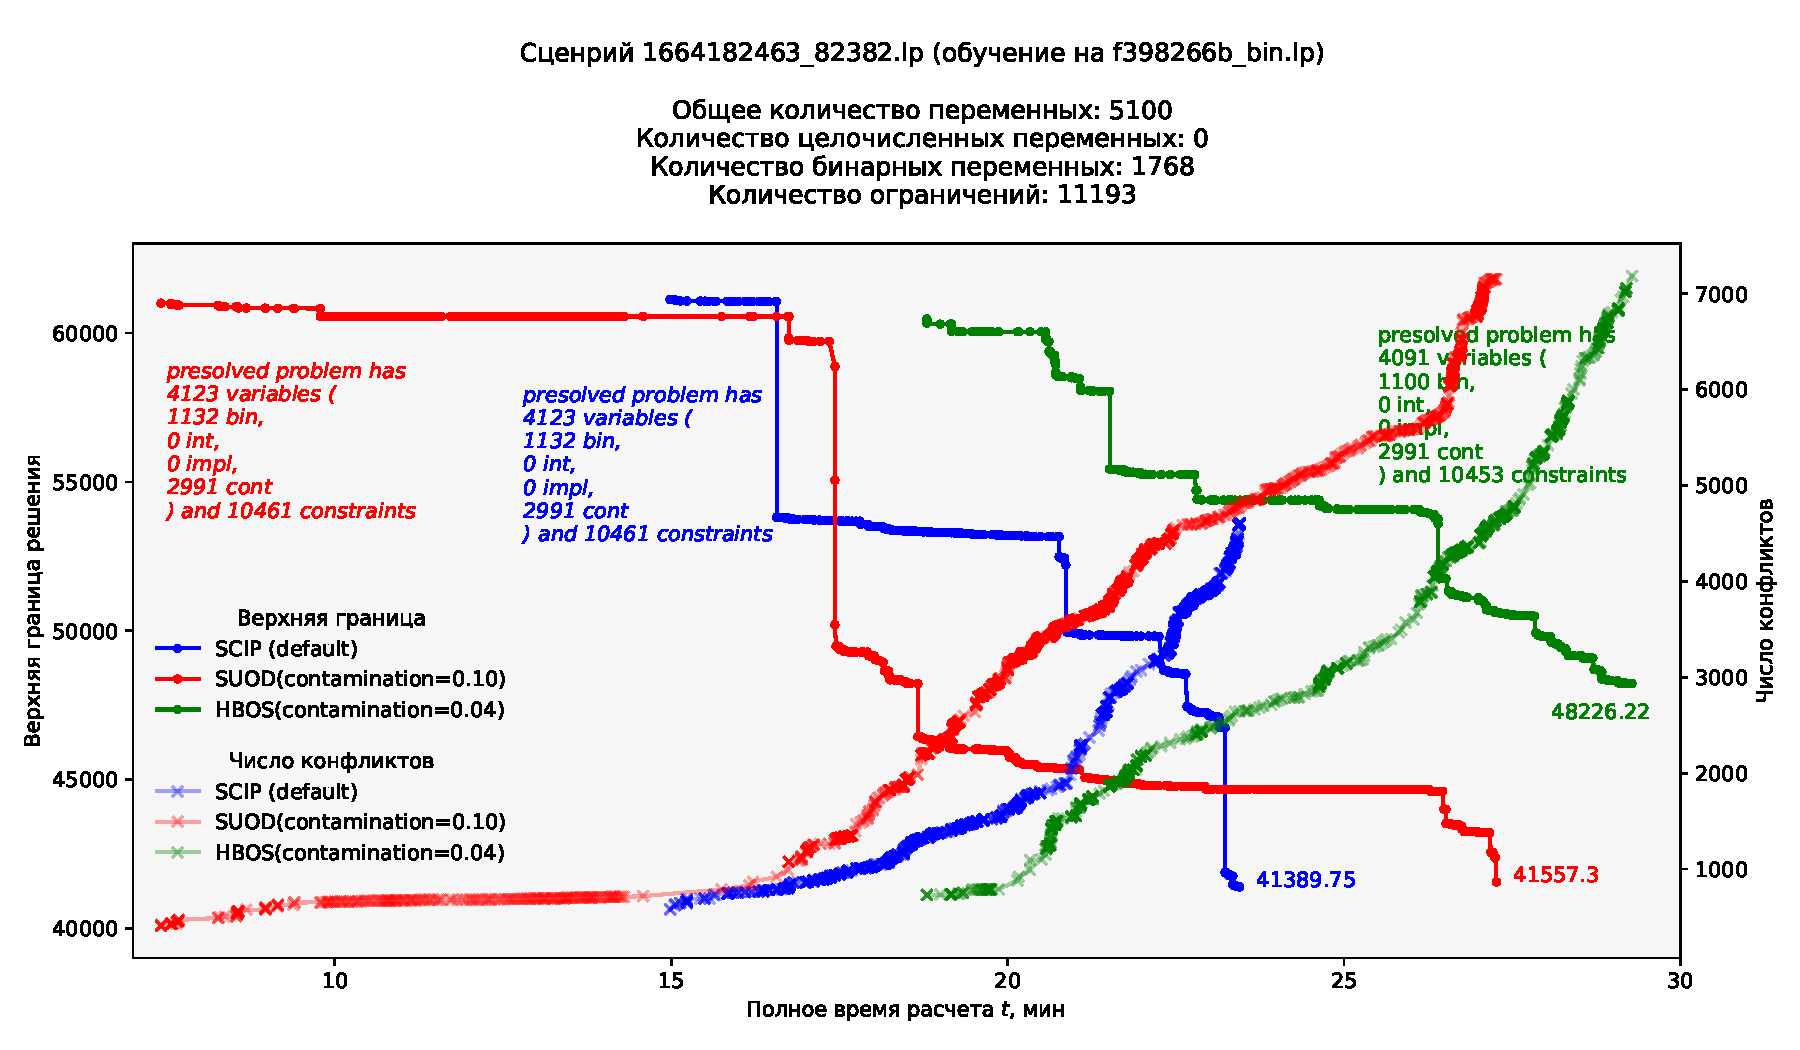
\includegraphics[scale=0.58]{figures/1664182546_82382.pdf}
	\caption{ Сводка результатов вычислительных экспериментов на сценарии \\группы СОП \texttt{1664182546\_82382.lp} }\label{fig:1664182546_82382}
\end{figure}


\subsubsection{Синтетический сценарий \texttt{1664182533\_1587787.lp} с бинарными переменными}

\textbf{Статистика}\footnote{В скобках указана размерность задачи после шага пресолвинга с фиксацией, полученной с помощью ансамбля детекторов аномалий без подбора гиперпараметров детекторов}\vspace*{1mm}

Общее количество переменных: 4759 (3780)

Количество целочисленных переменных: 0 (0)

Количество бинарных переменных: 1701 (1063)

Количество ограничений: 10307 (9581)

lp-файл: \url{https://disk.yandex.ru/d/n0Dqn6pr6GK9mg}

Блок подавления подгруппы первичных эвристик низкой эффективности конфигурационного файла SCIP
\begin{lstlisting}[
title = {\sffamily Фрагмент файла scip.set. Сценарий 1664182533\_1587787.lp},
style = bash,
numbers = none
]
...
heuristics/adaptivediving/freq = -1
heuristics/fracdiving/freq = -1
heuristics/linesearchdiving/freq = -1
heuristics/objpscostdiving/freq = -1
heuristics/pscostdiving/freq = -1
heuristics/rootsoldiving/freq = -1
heuristics/veclendiving/freq = -1
\end{lstlisting}

На рис.~\ref{fig:1664182533_1587787} приведены результаты сравнительного анализа запусков i) решателя SCIP с настройками по умолчанию, ii) решателя SCIP на частично-заданном решении, полученном с помощью ансамбля детекторов аномалий, и iii) решателя SCIP на фиксации, подговтоленной с помощью изолированного детектора HBOS.

Здесь схема с настройками по умолчанию проигрывает схеме на частично-заданном решении, построенном с помощью ансамбля детекторов аномалий, и по времени расчета, и по значению целевой функции. Подбор параметра контаминации детектора HBOS как и в предыдущем случае не позволяет улучшить решение -- кривая <<замирает>> на асимптоте 52070.46.

Таким образом, в данном случае ансамбль детекторов аномалий с обреткой SUOD снижает временные издержки на получение решения и одновременно улучшает целевую функцию.

\textbf{Вывод по сценарию}: принимая во внимание, что ансамбль детекторов аномалий обучался лишь на одном сценарии группы ИКП, который существенно и с точки зрения размерности, и с точки зрения структуры матрицы ограничений отличается от сценария, на котором строился прогнгоз модели, допустимо говорить о трансфере/переносе шаблона, выявленного на сценарии \texttt{f398266b\_bin.lp} группы ИКП.

\begin{figure}[!h]
	\centering
%	\begin{mdframed}[backgroundcolor=gray!25,linecolor=gray!25]
	    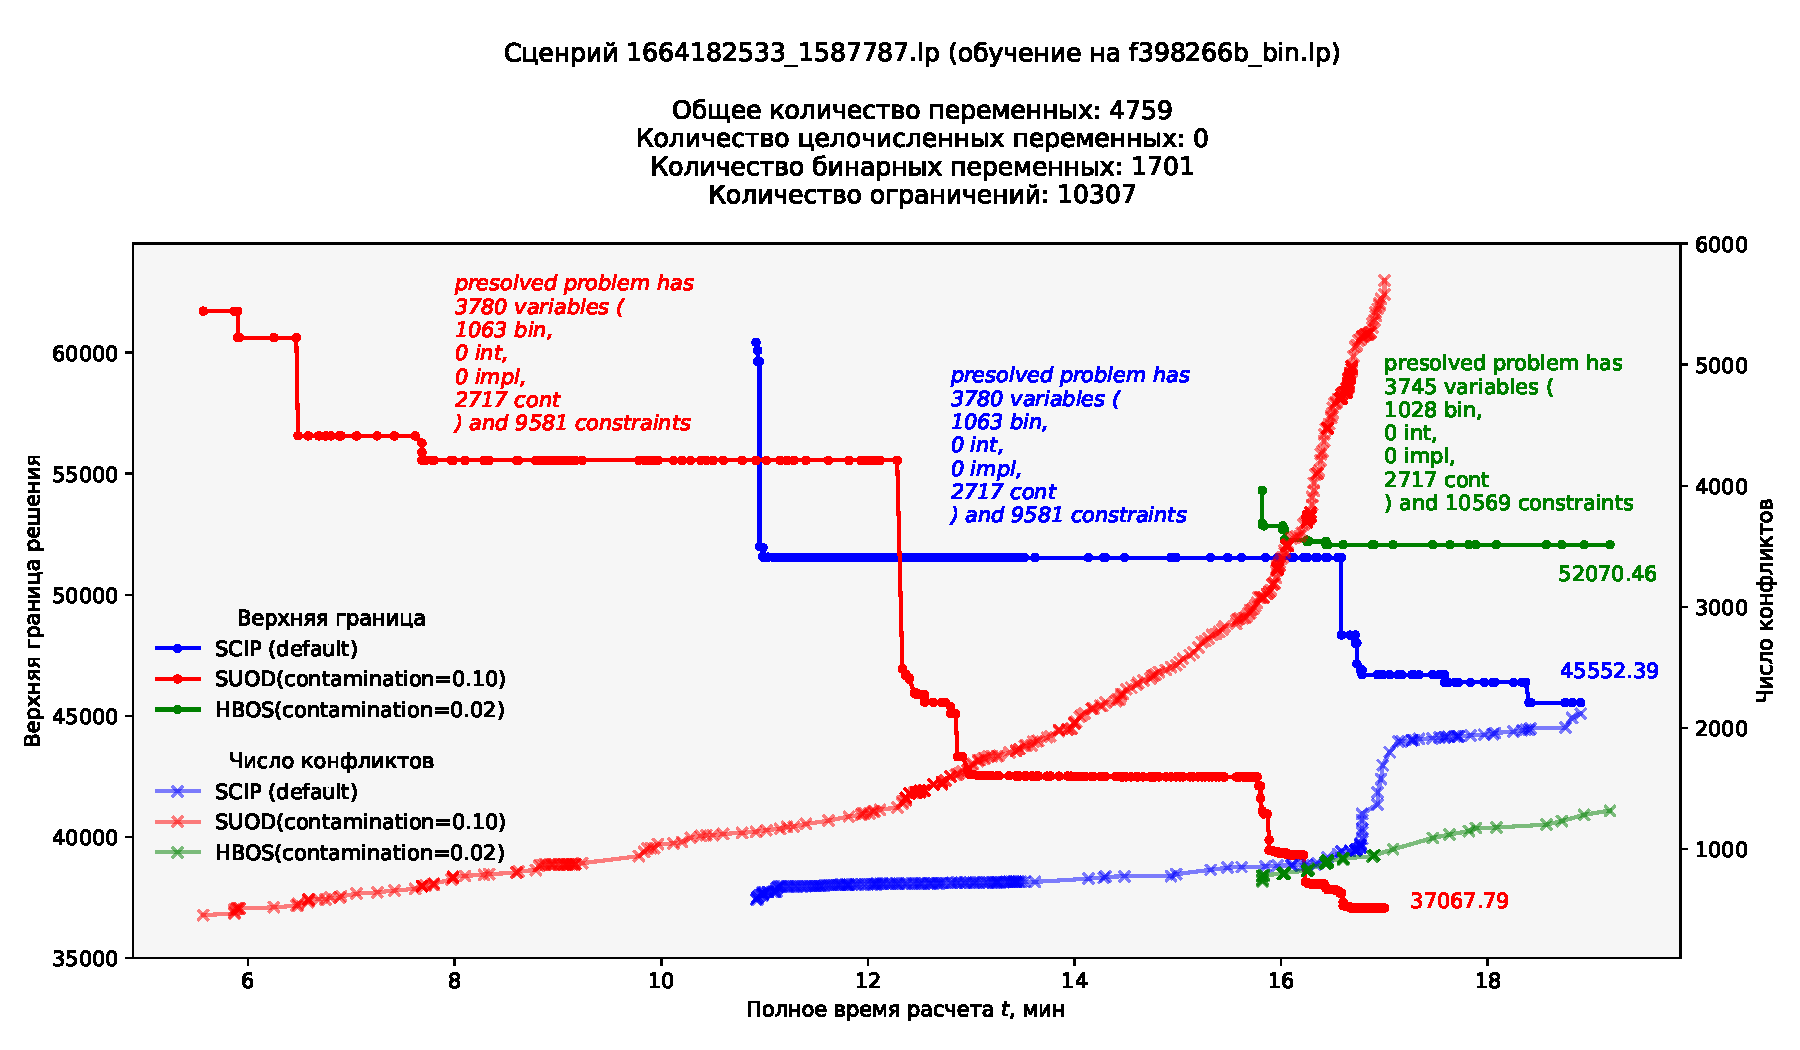
\includegraphics[scale=0.535]{figures/1664182533_1587787.pdf}
	    \caption{ Сводка результатов вычислительных экспериментов \\на сценарии группы СОП \texttt{1664182533\_1587787.lp} }\label{fig:1664182533_1587787}
%	\end{mdframed}
\end{figure}


\subsubsection{Синтетический сценарий \texttt{1664182480\_4326847.lp} с бинарными переменными}

\textbf{Статистика}\footnote{В скобках указана размерность задачи после шага пресолвинга с фиксацией, полученной с помощью ансамбля детекторов аномалий без подбора гиперпараметров детекторов}\vspace*{1mm}

Общее количество переменных: 7123 (6445)

Количество целочисленных переменных: 0 (0)

Количество бинарных переменных: 1548 (1324)

Количество ограничений: 17696 (16805)

lp-файл: \url{https://disk.yandex.ru/d/f_6GH9mzzxAGQg}

Блок подавления подгруппы первичных эвристик низкой эффективности конфигурационного файла SCIP
\begin{lstlisting}[
title = {\sffamily Фрагмент файла scip.set. Сценарий 1664182480\_4326847.lp},
style = bash,
numbers = none
]
...
heuristics/adaptivediving/freq = -1
heuristics/fracdiving/freq = -1
heuristics/linesearchdiving/freq = -1
heuristics/objpscostdiving/freq = -1
heuristics/pscostdiving/freq = -1
heuristics/rootsoldiving/freq = -1
heuristics/veclendiving/freq = -1
\end{lstlisting}

На рис.~\ref{fig:1664182480_4326847} приведены результаты сравнительного анализа запусков i) решателя SCIP с настройками по умолчанию и ii) решателя SCIP на фиксации, подговтоленной с помощью изолированного детектора HBOS.

На рассматриваемом сценарии получить решение с помощью ансамбля детекторов аномалий за отведенное для поиска время не удалось, однако, изолированный детектор HBOS с подобранным параметром контаминации смог выйти на значение целевой функции 53682.08. Это решение проигрывает решению, полученному с помощью SCIP базовой конфигурации (47245.97), но тем не менее указывает жизнеспособность концепции использования стратегии обнаружения аномалий для построения частично-заданного решения на фиксациях с подбором параметра контаминации детекторов.

\textbf{Вывод по сценарию}: принимая во внимание, что ансамбль детекторов аномалий обучался лишь на одном сценарии группы ИКП, который существенно и с точки зрения размерности, и с точки зрения структуры матрицы ограничений отличается от сценария, на котором строился прогнгоз модели, допустимо говорить о трансфере/переносе шаблона, выявленного на сценарии \texttt{f398266b\_bin.lp} группы ИКП.


\begin{figure}[!h]
	\centering
	\includegraphics[scale=0.58]{figures/1664182480\_4326847.pdf}
	\caption{ Сводка результатов вычислительных экспериментов \\на сценарии группы СОП \texttt{1664182480\_4326847.lp} }\label{fig:1664182480_4326847}
\end{figure}


\subsubsection{Синтетический сценарий \texttt{1664182523\_380519.lp} с бинарными переменными}

\textbf{Статистика}\footnote{В скобках указана размерность задачи после шага пресолвинга с фиксацией, полученной с помощью ансамбля детекторов аномалий без подбора гиперпараметров детекторов}\vspace*{1mm}

Общее количество переменных: 4578

Количество целочисленных переменных: 0

Количество бинарных переменных: 1331

Количество ограничений: 10722

lp-файл: \url{https://disk.yandex.ru/d/i-FhZ9LD8ToeXg}

Блок подавления подгруппы первичных эвристик низкой эффективности конфигурационного файла SCIP
\begin{lstlisting}[
title = {\sffamily Фрагмент файла scip.set. Сценарий 1664182523\_380519.lp},
style = bash,
numbers = none
]
...
heuristics/adaptivediving/freq = -1
heuristics/fracdiving/freq = -1
heuristics/linesearchdiving/freq = -1
heuristics/objpscostdiving/freq = -1
heuristics/pscostdiving/freq = -1
heuristics/rootsoldiving/freq = -1
heuristics/veclendiving/freq = -1
\end{lstlisting}

На рис.~\ref{fig:1664182523_380519} приведены результаты сравнительного анализа запусков i) решателя SCIP с настройками по умолчанию, и ii) решателя SCIP на частично-заданном решении, полученном с помощью ансамбля детекторов аномалий.

Здесь ансамбль детекторов аномалий выигрывает 2.78 минуты при целевой функции, значение которой практически не отличается от значения целевой функции в решении, полученном с помощью решателя SCIP базовой конфигурации.

\begin{figure}[!h]
	\centering
	\includegraphics[scale=0.58]{figures/1664182523\_380519.pdf}
	\caption{ Сводка результатов вычислительных экспериментов \\на сценарии группы СОП \texttt{1664182523\_380519.lp} }\label{fig:1664182523_380519}
\end{figure}

\textbf{Вывод по сценарию}: принимая во внимание, что ансамбль детекторов аномалий обучался лишь на одном сценарии группы ИКП, который существенно и с точки зрения размерности, и с точки зрения структуры матрицы ограничений отличается от сценария, на котором строился прогнгоз модели, допустимо говорить о трансфере/переносе шаблона, выявленного на сценарии \texttt{f398266b\_bin.lp} группы ИКП.

\subsection{Концепт построения матрицы признакового описания объекта для задачи выбора стратегии поиска решения}

Каждую проблему из набора решаем различными стратегиями (HiGHS с настройками по умолчанию, SCIP с настройками по умолчанию, ZyOpt 1-ой конфигурации, ZyOpt 2-ой конфигурации и т.д.). Затем выбираем наиболее эффективную стратегию для каждой проблемы. Это и будет разметка. Проблему отображаем на вектор-строку матрицы признакового описания объекта и в итого получаем матрицу плана. Теперь требуется решить задачу мультиклассовой классификации. Классификатор будет возвращать вероятность принадлежности экземпляра классам. Выбираем класс с наибольшей вероятностью. Таким образом можно связать стратегию поиска решения с представлением проблемы и проранжировать стратегии. Начинаем с самой эффективной, а потом по убывающей. 

\section{Влияние правой границы переменных на эффективность процедуры поиска решения}

Гипотеза состоит в том, что если правую границу переменных ограничить каким-то образом, то это должно положительно сказаться на времени поиска первого допустимого решения. 

На проблемах \verb|2023_03_ONPZ_1615.lp| и \verb|2023_01_ONPZ_1591.lp| полезно бесконечные правые границы купировать значением $ 100 \cdot \max(\text{relax\_sol}) $. Однако для проблемы \verb|2023_03_ONPZ_1615.lp| эффективно ограничение бинарных и целочисленных переменных значением $ (2 \cdot UB_{relax}) $ (первое допустимое решение находится за 300 сек.), а для проблемы \verb|2023_01_ONPZ_1591.lp| -- $ (2 \cdot UB_{relax} + 10) $ (первое допустимое решение находится за 543 сек.). При чем, если бинарные и целочисленные переменные проблемы \verb|2023_03_ONPZ_1615.lp| ограничить значением $ (2 \cdot UB_{relax} + 10) $, то решение не удастся найти и за 3600 сек.



\section{Описание вычислительных экспериментов на сценариях группы ИКП}\label{sec:ikp}

На всех сценариях группы ИКП (как с бинарными переменными, так и без них) решения удавалось найти с помощью \emph{метаконфигурации} (см. раздел~\ref{sec:ikp_bins}), включающей прием подавления подгруппы первичных эвристик низкой эффективности и процедуру построения частично-заданного решения на фиксациях (для нулевых бинарных и целочисленных переменных). 

\subsection{Поиск решения на сценариях \emph{без} бинарных переменных. \\Метаконфигурации SUH,  FZBIVSUHPB и ансамбль детекторов аномалий}

Метаконфигурация\footnote{Под метаконфигурацией понимается совокупность конфигурации решателя и набора эвристических приемов} SUH (Suppress Useless Heuristics) процедуры поиска решения сводится к приему подавления подгруппы первичных эвристик низкой эффективности.

\remark{
Решение получено без доменно-ориентированных эвристик, <<теплого>> старта и подбора параметров решателя
}

Конфигурация решателя SCIP для всех сценариев группы ИКП (без бинарных переменных) имеет вид
\begin{lstlisting}[
	title = {\sffamily scip.set. Сценарии группы ИКП без бинарных переменных},
	style = bash,
	numbers = none,
	]
	# критерии останова и перезапуска
	limits/time = 7200
	limits/gap = 0.02  # решение останавливается при зазоре <= 2%
	
	# подавление подгруппы первичных эвристик низкой эффективности
	heuristics/farkasdiving/freq = -1
	heuristics/feaspump/freq = -1
	heuristics/randrounding/freq = -1
	heuristics/shiftandpropagate/freq = -1
	heuristics/shifting/freq = -1
\end{lstlisting}

Сводка результатов вычислительных экспериментов доступна по ссылке \url{https://docs.google.com/document/d/1V9fZLT9cXkbVQ5BvMCwzKrAiASZ2v4-01Z68jVBZUBU/edit?usp=sharing}.

\subsubsection{Сценарий \texttt{F398266B} без бинарных переменных}

\textbf{Статистика}\vspace*{1mm}

Общее количество переменных: 774901

Количество целочисленных переменных: 172449

Количество бинарных переменных: 0

Количество ограничений: 650263

lp-файл: \url{https://disk.yandex.ru/d/o_eAb9475u5ueg}

\vspace*{5mm}\textbf{Анализ решения}\vspace*{1mm}

Пул решений задачи был найден с помощью следующих первичных эвристик:
\begin{itemize}
	\item INTSHIFING,
	
	\item RENS.
\end{itemize}

Файл решения задачи (метаконфигурация SUH) доступен по ссылке \url{https://disk.yandex.ru/d/URRnZ8soTaJEgQ}

Файл статистической сводки (метаконфигурация SUH) доступен по ссылке \url{https://disk.yandex.ru/d/N2tfhj1N6RczzA}

Файл решения задачи (метаконфигурация FZBIVSUHPB) доступен по ссылке \url{https://disk.yandex.ru/d/-y7p5FyJyYirkw}

Файл статистической сводки (метаконфигурация FZBIVSUHPB) доступен по ссылке \url{https://disk.yandex.ru/d/1JaMC9aFjubDbA}

\vspace*{3mm}
\textbf{Вывод по сценарию}: описанная выше метаконфигурация SUH приводит к решению задачи, которое оказывается по отношению к результату на доменно-ориентированных эвристиках (\verb|USE_RECALCULATION_ON_FLOW=true|) для последнего решения из пула допустимых целочисленных решений (ОС Linux Centos 7) на 1.063\% лучше в смысле целевой функции и на 10.20\% -- в смысле временных издержек (\pic{fig:summary_f398266b}). 

Метаконфигурация FZBIVSUHPB (подробнее в разделе~\ref{sec:ikp_bins}) по отношению к тому же результату на доменно-ориентированных эвристиках дает решение задачи, которое на 1.155\% лучше в смысле целевой функции и на 65.27\% -- в смысле временных издержек (\tblref{tab:f398266b_wo_bins}).

Синим цветом обозначен выигрыш в процентах.

{
	%\rowcolors{2}{white}{lightgray!15}
	\begin{table}[!h]
		\centering
		\caption{Сводка результатов анализа эффективности \\метаконфигураций SUH и FZBIVSUHPB. Сценарий \texttt{f398266b} без бинарных переменных}
		\begin{tabular}{ p{2.5cm} p{3.3cm} p{3.4cm} }
			\emph{Способ} & \emph{Полное время расчета, мин} & \emph{Верхняя граница решения, $ \times 10^{10} $} \\
			\hline\hline\\[-3.5mm]
			{CBC+DOH} & 21.38 & $ 5.905048 $ \\
			\hline
			SCIP+SUH & 19.27 {\color{blue} $\ +9.87 $\%} & $ 5.842154 $ {\color{blue} $\ +1.065 $\%} \\
			\hline
			SCIP+FZB... & 9.43 {\color{blue} $\ +55.89 $\%} & $ 5.836815 $ {\color{blue} $\ +1.155 $\%} \\
		\end{tabular}\label{tab:f398266b_wo_bins}
	\end{table}
}

\begin{figure}[!h]
	\centering
	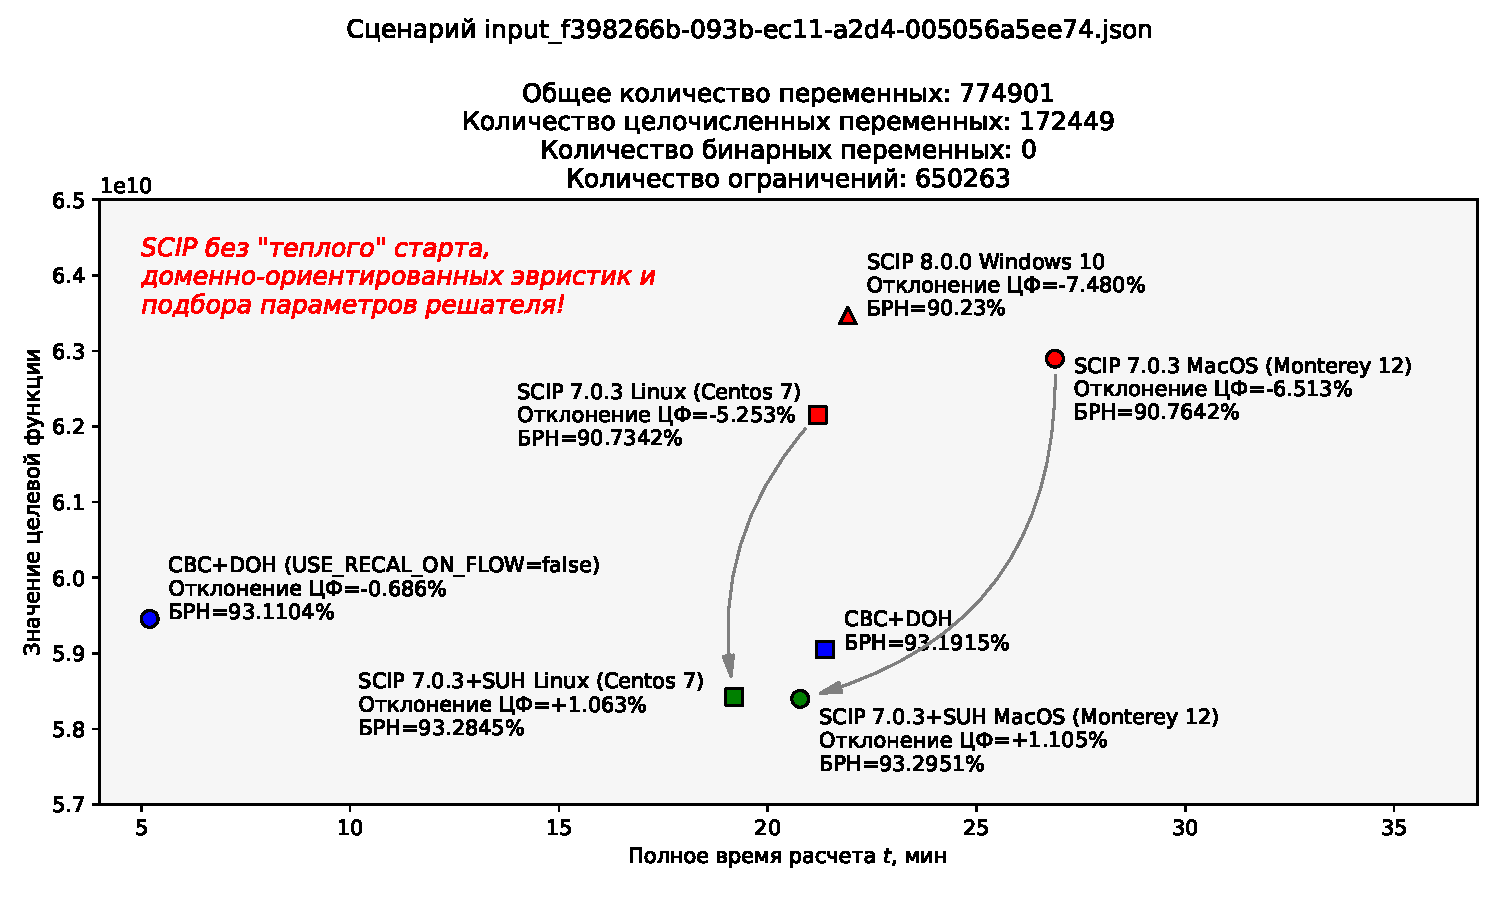
\includegraphics[scale=0.6]{figures/summary_f398266b.pdf}
	\caption{Сводка результатов анализа эффективности метаконфигурации SUH. \\Сценарий \texttt{f398266b} без бинарных переменных}\label{fig:summary_f398266b}
\end{figure}


\subsubsection{Сценарий \texttt{50197DF7} без бинарных переменных}

\textbf{Статистика}\vspace*{1mm}

Общее количество переменных: 718464

Количество целочисленных переменных: 159332

Количество бинарных переменных: 0

Количество ограничений: 595797

lp-файл: \url{https://disk.yandex.ru/d/KO_xj9dkgUdcog}

\vspace*{5mm}\textbf{Анализ решения}\vspace*{1mm}

Пул решений задачи был найден с помощью следующих первичных эвристик:
\begin{itemize}
	\item INTSHIFING,
	
	\item RENS.
\end{itemize}

Файл решения задачи (метаконфигурация SUH) доступен по ссылке \url{https://disk.yandex.ru/d/R4B1fkTx-nE3tg}

Файл статистической сводки (метаконфигурация SUH) доступен по ссылке \url{https://disk.yandex.ru/d/BLvUmZ43vtMFKg}

Файл решения задачи (метаконфигурация FZBIVSUHPB) доступен по ссылке \url{https://disk.yandex.ru/d/yMFLr-6mLfdPAw}

Файл статистической сводки (метаконфигурация FZBIVSUHPB) доступен по ссылке \url{https://disk.yandex.ru/d/XiRSvteL9xC4pg}

\vspace*{3mm}
\textbf{Вывод по сценарию}: описанная выше метаконфигурация SUH приводит к решению задачи, которое оказывается по отношению к результату на доменно-ориентированных эвристиках (\verb|USE_RECALCULATION_ON_FLOW=true|) для последнего решения из пула допустимых целочисленных решений (ОС Linux Centos 7) на 1.25\% лучше в смысле целевой функции и на 46.43\% -- в смысле временных издержек (\pic{fig:summary_50197df7}). 

Метаконфигурация FZBIVSUHPB (подробнее в разделе~\ref{sec:ikp_bins}) по отношению к тому же результату на доменно-ориентированных эвристиках дает решение задачи, которое на 1.191\% лучше в смысле целевой функции и на 82.13\% -- в смысле временных издержек (\tblref{tab:50197df7_wo_bins}).

Синим цветом обозначен выигрыш в процентах.

{
	%\rowcolors{2}{white}{lightgray!15}
	\begin{table}[!h]
		\centering
		\caption{Сводка результатов анализа эффективности \\метаконфигураций SUH и FZBIVSUHPB. Сценарий \texttt{50197df7} без бинарных переменных}
		\begin{tabular}{ p{2.5cm} p{3.3cm} p{3.4cm} }
			\emph{Способ} & \emph{Полное время расчета, мин} & \emph{Верхняя граница решения, $ \times 10^{10} $} \\
			\hline\hline\\[-3.5mm]
			{CBC+DOH} & 18.35 & $ 3.585532 $ \\
			\hline
			SCIP+SUH & 9.83 {\color{blue} $\ +46.43 $\%} & $ 3.540567 $ {\color{blue} $\ +1.252 $\%} \\
			\hline
			SCIP+FZB... & 3.28 {\color{blue} $\ +82.13 $\%} & $ 3.542843 $ {\color{blue} $\ +1.191 $\%} \\
		\end{tabular}\label{tab:50197df7_wo_bins}
	\end{table}
}

\begin{figure}[!h]
	\centering
	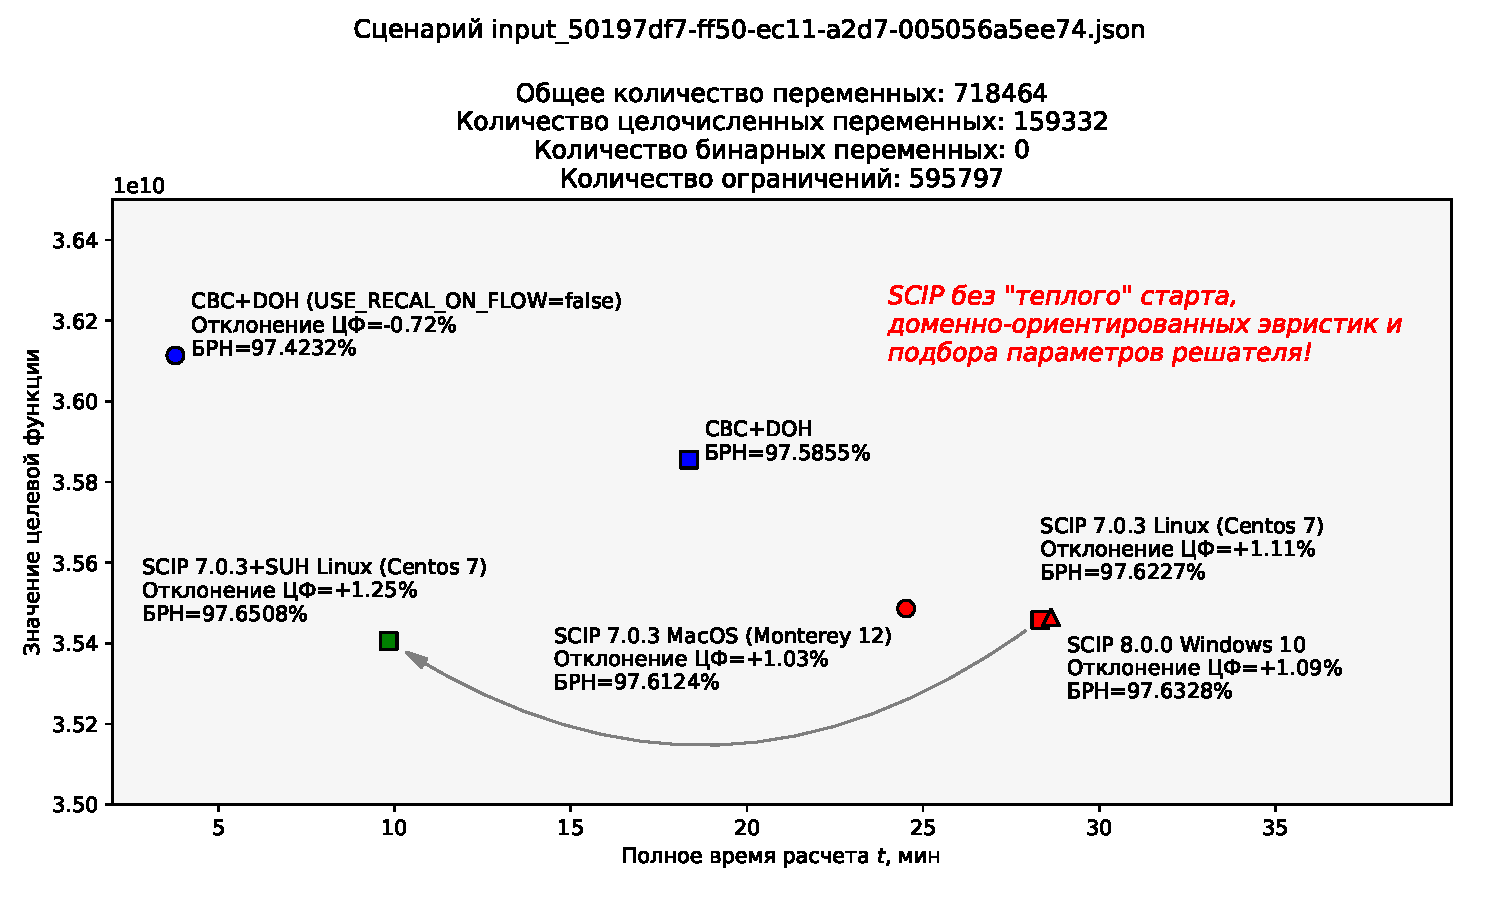
\includegraphics[scale=0.6]{figures/summary_50197df7.pdf}
	\caption{Сводка результатов анализа эффективности метаконфигурации SUH. \\Сценарий \texttt{50197df7} без бинарных переменных}\label{fig:summary_50197df7}
\end{figure}

\subsubsection{Сценарий \texttt{7FAC4231} без бинарных переменных}

\textbf{Статистика}\vspace*{1mm}

Общее количество переменных: 737585

Количество целочисленных переменных: 147789

Количество бинарных переменных: 0

Количество ограничений: 540018

lp-файл: \url{https://disk.yandex.ru/d/qiZAmraUNK1Peg}

\vspace*{5mm}\textbf{Анализ решения}\vspace*{1mm}

Пул решений задачи был найден с помощью следующих первичных эвристик:
\begin{itemize}
	\item INTSHIFING,
	
	\item RENS.
\end{itemize}

Файл решения задачи (метаконфигурация SUH) доступен по ссылке \url{https://disk.yandex.ru/d/20NeMuQ7NF_ccA}

Файл статистической сводки (метаконфигурация SUH) доступен по ссылке \url{https://disk.yandex.ru/d/QxE0HoREHzgHQQ}

Файл решения задачи (метаконфигурация FZBIVSUHPB) доступен по ссылке \url{https://disk.yandex.ru/d/FHZGj_Kyg8dDiw}

Файл статистической сводки (метаконфигурация FZBIVSUHPB) доступен по ссылке \url{https://disk.yandex.ru/d/8H1vw6zkQS7DAg}

\vspace*{3mm}
\textbf{Вывод по сценарию}: описанная выше метаконфигурация SUH приводит к решению задачи, которое оказывается по отношению к результату на доменно-ориентированных эвристиках (\verb|USE_RECALCULATION_ON_FLOW=true|) для последнего решения из пула допустимых целочисленных решений (ОС Linux Centos 7) на 5.22\% лучше в смысле целевой функции и на 27.10\% -- в смысле временных издержек (\pic{fig:summary_7fac4231}).

Метаконфигурация FZBIVSUHPB (подробнее в разделе~\ref{sec:ikp_bins}) по отношению к тому же результату на доменно-ориентированных эвристиках дает решение задачи, которое на 5.452\% лучше в смысле целевой функции и на 90.16\% -- в смысле временных издержек (\tblref{tab:7fac4231_wo_bins}).

Синим цветом обозначен выигрыш в процентах.

{
	%\rowcolors{2}{white}{lightgray!15}
	\begin{table}[!h]
		\centering
		\caption{Сводка результатов анализа эффективности \\метаконфигураций SUH и FZBIVSUHPB. Сценарий \texttt{7fac4231} без бинарных переменных}
		\begin{tabular}{ p{2.5cm} p{3.3cm} p{3.4cm} }
			\emph{Способ} & \emph{Полное время расчета, мин} & \emph{Верхняя граница решения, $ \times 10^{10} $} \\
			\hline\hline\\[-3.5mm]
			{CBC+DOH} & 16.05 & $ 1.087609 $ \\
			\hline
			SCIP+SUH & 11.67 {\color{blue} $\ +27.29 $\%} & $ 1.030866 $ {\color{blue} $\ +5.222 $\%} \\
			\hline
			SCIP+FZB... & 3.58 {\color{blue} $\ +77.69 $\%} & $ 1.028349 $ {\color{blue} $\ +5.452 $\%} \\
		\end{tabular}\label{tab:7fac4231_wo_bins}
	\end{table}
}

\begin{figure}[!h]
	\centering
	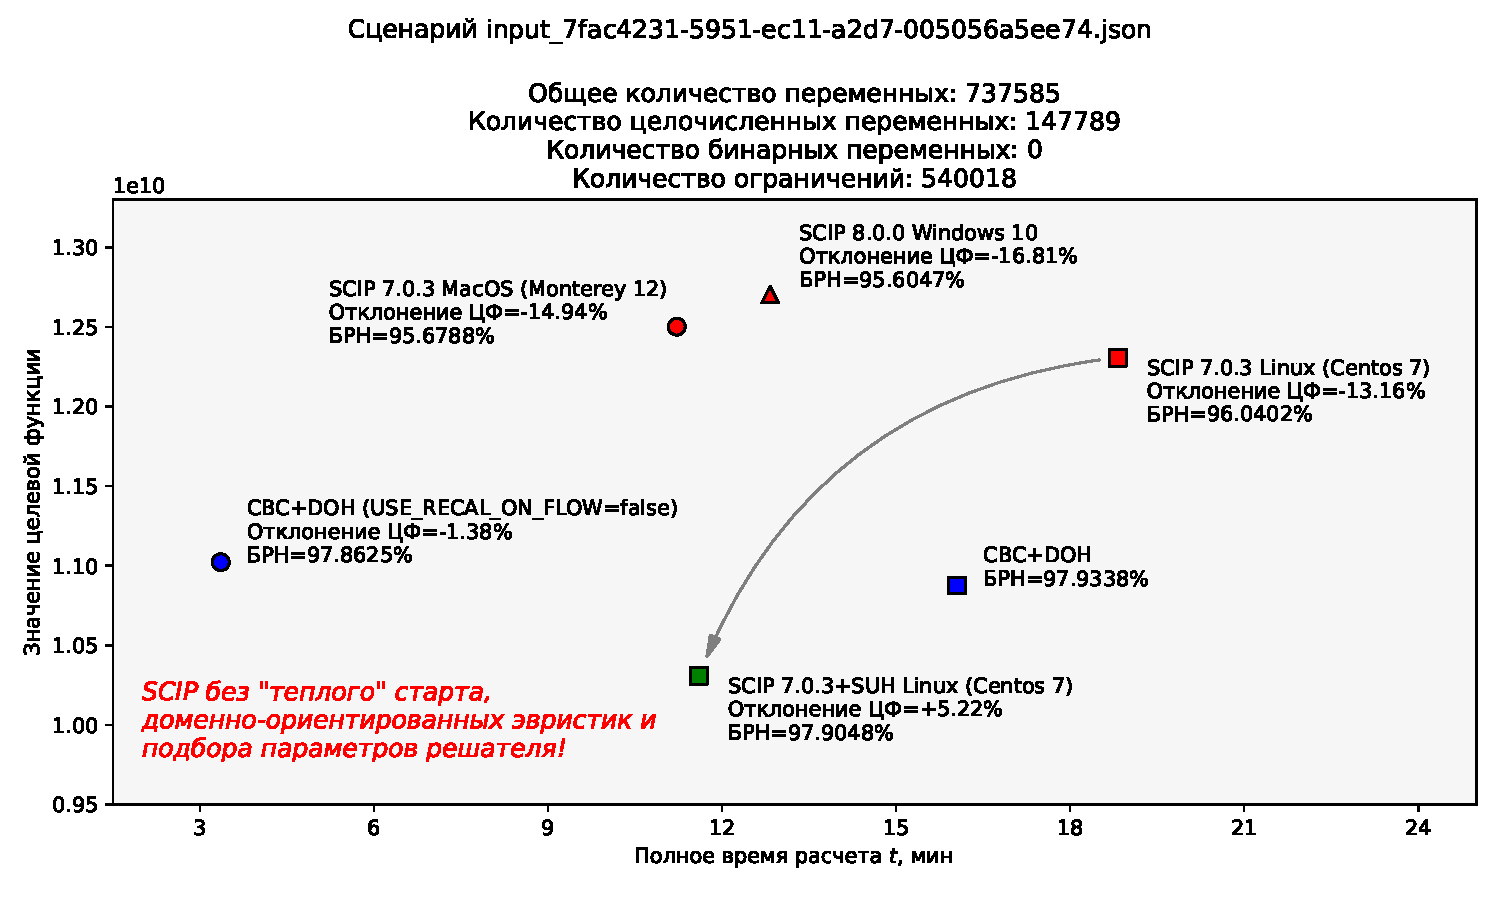
\includegraphics[scale=0.6]{figures/summary_7fac4231.pdf}
	\caption{Сводка результатов анализа эффективности метаконфигурации SUH. \\Сценарий \texttt{7fac4231} без бинарных переменных}\label{fig:summary_7fac4231}
\end{figure}

\subsubsection{Сценарий \texttt{CA485A55} без бинарных переменных}

\textbf{Статистика}\vspace*{1mm}

Общее количество переменных: 718601

Количество целочисленных переменных: 140858

Количество бинарных переменных: 0

Количество ограничений: 514229

lp-файл: \url{https://disk.yandex.ru/d/iSP6xrh4K_wHEQ}

\vspace*{5mm}\textbf{Анализ решения}\vspace*{1mm}

Пул решений задачи был найден с помощью следующих первичных эвристик:
\begin{itemize}
	\item INTSHIFING,
	
	\item RENS.
\end{itemize}

Файл решения задачи (метаконфигурация SUH) доступен по ссылке \url{https://disk.yandex.ru/d/_WzkmgoueNb2Bg}

Файл решения задачи (метаконфигурация FZBIVSUHPB) доступен по ссылке \url{https://disk.yandex.ru/d/sLUW5IxmpMBpcw}

Файл статистической сводки (метаконфигурация FZBIVSUHPB) доступен по ссылке \url{https://disk.yandex.ru/d/3Ls6QrAWVUMdZw}

\vspace*{3mm}
\textbf{Вывод по сценарию}: описанная выше метаконфигурация SUH приводит к решению задачи, которое оказывается по отношению к результату на доменно-ориентированных эвристиках (\verb|USE_RECALCULATION_ON_FLOW=true|) для последнего решения из пула допустимых целочисленных решений (ОС Linux Centos 7) на 0.683\% лучше в смысле целевой функции и на 46.48\% -- в смысле временных издержек (\pic{fig:summary_ca485a55}).

Метаконфигурация FZBIVSUHPB (подробнее в разделе~\ref{sec:ikp_bins}) по отношению к тому же результату на доменно-ориентированных эвристиках дает решение задачи, которое на 1.244\% лучше в смысле целевой функции и на 88.53\% -- в смысле временных издержек (\tblref{tab:ca485a55_wo_bins}).

Синим цветом обозначен выигрыш в процентах.

{
	%\rowcolors{2}{white}{lightgray!15}
	\begin{table}[!h]
		\centering
		\caption{Сводка результатов анализа эффективности \\метаконфигураций SUH и FZBIVSUHPB. Сценарий \texttt{ca485a55} без бинарных переменных}
		\begin{tabular}{ p{2.5cm} p{3.3cm} p{3.4cm} }
			\emph{Способ} & \emph{Полное время расчета, мин} & \emph{Верхняя граница решения, $ \times 10^{10} $} \\
			\hline\hline\\[-3.5mm]
			{CBC+DOH} & 20.05 & $ 4.597048 $ \\
			\hline
			SCIP+SUH & 10.73 {\color{blue} $\ +46.48 $\%} & $ 4.565579 $ {\color{blue} $\ +0.683 $\%} \\
			\hline
			SCIP+FZB... & 4.34 {\color{blue} $\ +78.35 $\%} & $ 4.539819 $ {\color{blue} $\ +1.244 $\%} \\
		\end{tabular}\label{tab:ca485a55_wo_bins}
	\end{table}
}

\begin{figure}[!h]
	\centering
	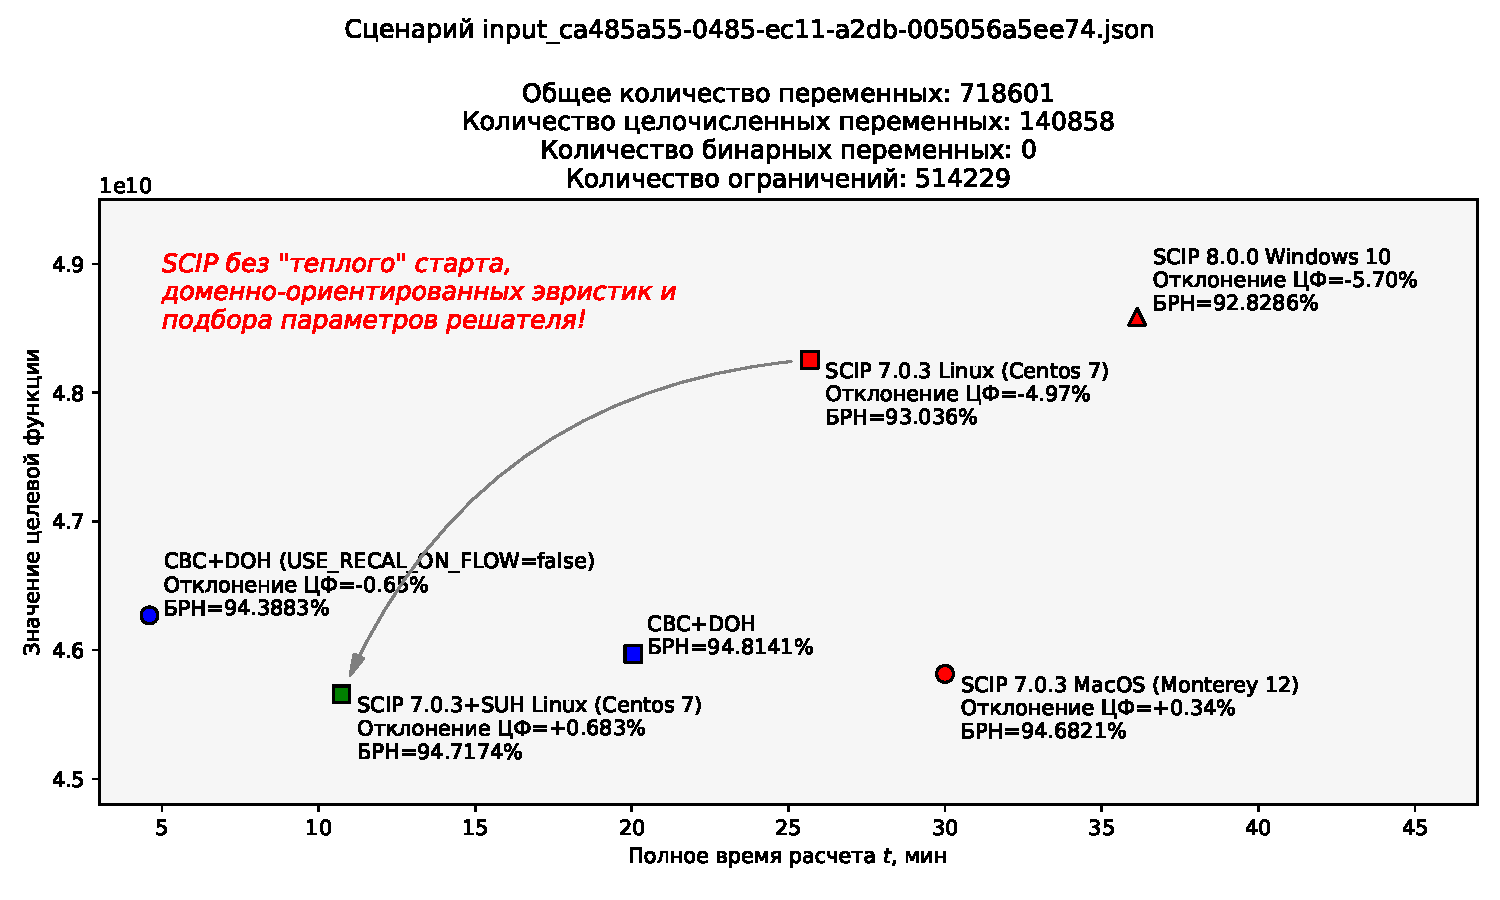
\includegraphics[scale=0.6]{figures/summary_ca485a55.pdf}
	\caption{Сводка результатов анализа эффективности метаконфигурации SUH. \\Сценарий \texttt{ca485a55} без бинарных переменных}\label{fig:summary_ca485a55}
\end{figure}

\subsubsection{Сценарий \texttt{276} без бинарных переменных}

\textbf{Статистика}\vspace*{1mm}

Общее количество переменных: 809224

Количество целочисленных переменных: 162562

Количество бинарных переменных: 0

Количество ограничений: 602190

lp-файл: \url{https://disk.yandex.ru/d/QaS5kd7VRZQ66A}

\vspace*{5mm}\textbf{Анализ решения}\vspace*{1mm}

Пул решений задачи был найден с помощью следующих первичных эвристик:
\begin{itemize}
	\item INTSHIFING,
	
	\item RENS.
\end{itemize}

Файл решения задачи (метаконфигурация SUH) доступен по ссылке \url{https://disk.yandex.ru/d/M2V88djiiGM5PA}

Файл решения задачи (метаконфигурация FZBIVSUHPB) доступен по ссылке \url{https://disk.yandex.ru/d/G0ustAVT6I9CeA}

Файл статистической сводки (метаконфигурация FZBIVSUHPB) доступен по ссылке \url{https://disk.yandex.ru/d/YBXB5GCECJiBIA}

\vspace*{3mm}
\textbf{Вывод по сценарию}: описанная выше метаконфигурация SUH приводит к решению задачи, которое оказывается по отношению к результату на доменно-ориентированных эвристиках (\verb|USE_RECALCULATION_ON_FLOW=true|) для последнего решения из пула допустимых целочисленных решений (ОС Linux Centos 7) на 3.67\% лучше в смысле целевой функции и на 51.56\% -- в смысле временных издержек (\pic{fig:summary_276}).

Метаконфигурация FZBIVSUHPB (подробнее в разделе~\ref{sec:ikp_bins}) по отношению к тому же результату на доменно-ориентированных эвристиках дает решение задачи, которое на 4.86\% лучше в смысле целевой функции и на 78.35\% -- в смысле временных издержек (\tblref{tab:276_wo_bins}).

Синим цветом обозначен выигрыш в процентах.

{
	%\rowcolors{2}{white}{lightgray!15}
	\begin{table}[!h]
		\centering
		\caption{Сводка результатов анализа эффективности \\метаконфигураций SUH и FZBIVSUHPB. Сценарий \texttt{276} без бинарных переменных}
		\begin{tabular}{ p{2.5cm} p{3.3cm} p{3.4cm} }
			\emph{Способ} & \emph{Полное время расчета, мин} & \emph{Верхняя граница решения, $ \times 10^{10} $} \\
			\hline\hline\\[-3.5mm]
			{CBC+DOH} & 29.87 & $ 1.430789 $ \\
			\hline
			SCIP+SUH & 14.47 {\color{blue} $\ +51.56 $\%} & $ 1.378299 $ {\color{blue} $\ +3.669 $\%} \\
			\hline
			SCIP+FZB... & 3.95 {\color{blue} $\ +78.35 $\%} & $ 1.361368 $ {\color{blue} $\ +4.857 $\%} \\
		\end{tabular}\label{tab:276_wo_bins}
	\end{table}
}


\begin{figure}[!h]
	\centering
	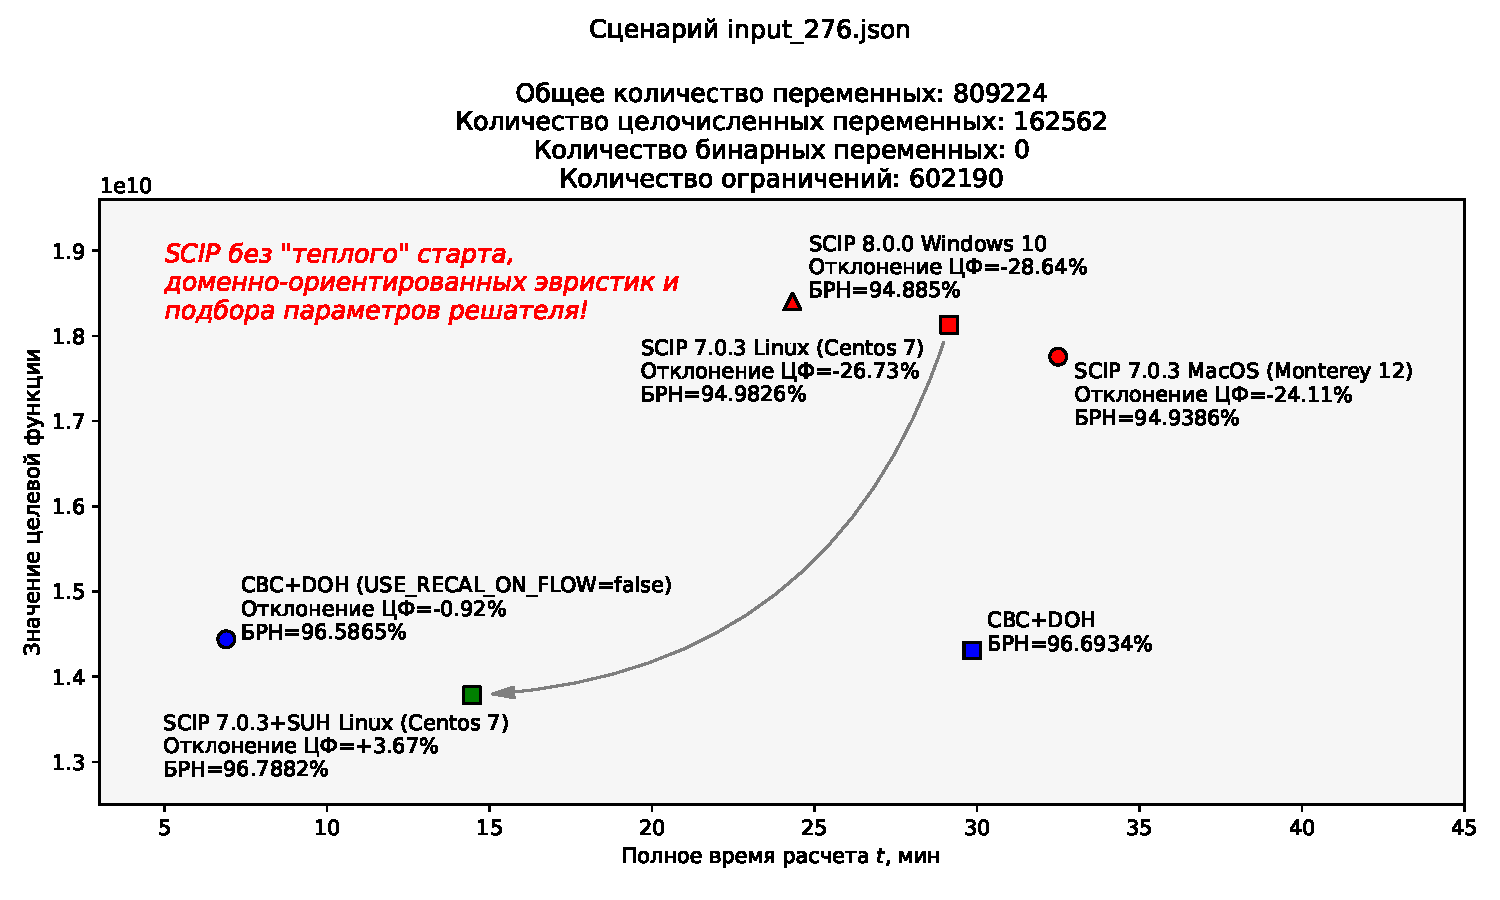
\includegraphics[scale=0.6]{figures/summary_276.pdf}
	\caption{Сводка результатов анализа эффективности метаконфигурации SUH. \\Сценарий \texttt{276} без бинарных переменных}\label{fig:summary_276}
\end{figure}

\subsubsection{Сценарий \texttt{337} без бинарных переменных}

\textbf{Статистика}\vspace*{1mm}

Общее количество переменных: 859075

Количество целочисленных переменных: 173622

Количество бинарных переменных: 0

Количество ограничений: 624327

lp-файл: \url{https://disk.yandex.ru/d/keyQLAagsD7Sbw}

\vspace*{5mm}\textbf{Анализ решения}\vspace*{1mm}

Пул решений задачи был найден с помощью следующих первичных эвристик:
\begin{itemize}
	\item INTSHIFING,
	
	\item RENS.
\end{itemize}

Файл решения задачи (метаконфигурация SUH) доступен по ссылке \url{https://disk.yandex.ru/d/ZUIEo3dDq77FjA}

Файл решения задачи (метаконфигурация FZBIVSUHPB) доступен по ссылке \url{https://disk.yandex.ru/d/0nUXIrIKuzqZlw}

Файл статистической сводки (метаконфигурация FZBIVSUHPB) доступен по ссылке \url{https://disk.yandex.ru/d/U0NCnMQN1akHUA}

\vspace*{3mm}
\textbf{Вывод по сценарию}: описанная выше метаконфигурация SUH приводит к решению задачи, которое оказывается по отношению к результату на доменно-ориентированных эвристиках (\verb|USE_RECALCULATION_ON_FLOW=true|) для последнего решения из пула допустимых целочисленных решений (ОС Linux Centos 7) на 22.12\% лучше в смысле целевой функции и на 18.32\% -- в смысле временных издержек (\pic{fig:summary_337}).

Метаконфигурация FZBIVSUHPB (подробнее в разделе~\ref{sec:ikp_bins}) по отношению к тому же результату на доменно-ориентированных эвристиках дает решение задачи, которое на 22.59\% лучше в смысле целевой функции и на 70.84\% -- в смысле временных издержек (\tblref{tab:337_wo_bins}).

Синим цветом обозначен выигрыш в процентах.

{
	%\rowcolors{2}{white}{lightgray!15}
	\begin{table}[!h]
		\centering
		\caption{Сводка результатов анализа эффективности \\метаконфигураций SUH и FZBIVSUHPB. Сценарий \texttt{337} без бинарных переменных}
		\begin{tabular}{ p{2.5cm} p{3.3cm} p{3.4cm} }
			\emph{Способ} & \emph{Полное время расчета, мин} & \emph{Верхняя граница решения, $ \times 10^{10} $} \\
			\hline\hline\\[-3.5mm]
			{CBC+DOH} & 20.85 & $ 3.825042 $ \\
			\hline
			SCIP+SUH & 17.03 {\color{blue} $\ +18.32 $\%} & $ 2.978782 $ {\color{blue} $\ +22.123 $\%} \\
			\hline
			SCIP+FZB... & 6.08 {\color{blue} $\ +70.84 $\%} & $ 2.961019 $ {\color{blue} $\ +22.588 $\%} \\
		\end{tabular}\label{tab:337_wo_bins}
	\end{table}
}


\begin{figure}[!h]
	\centering
	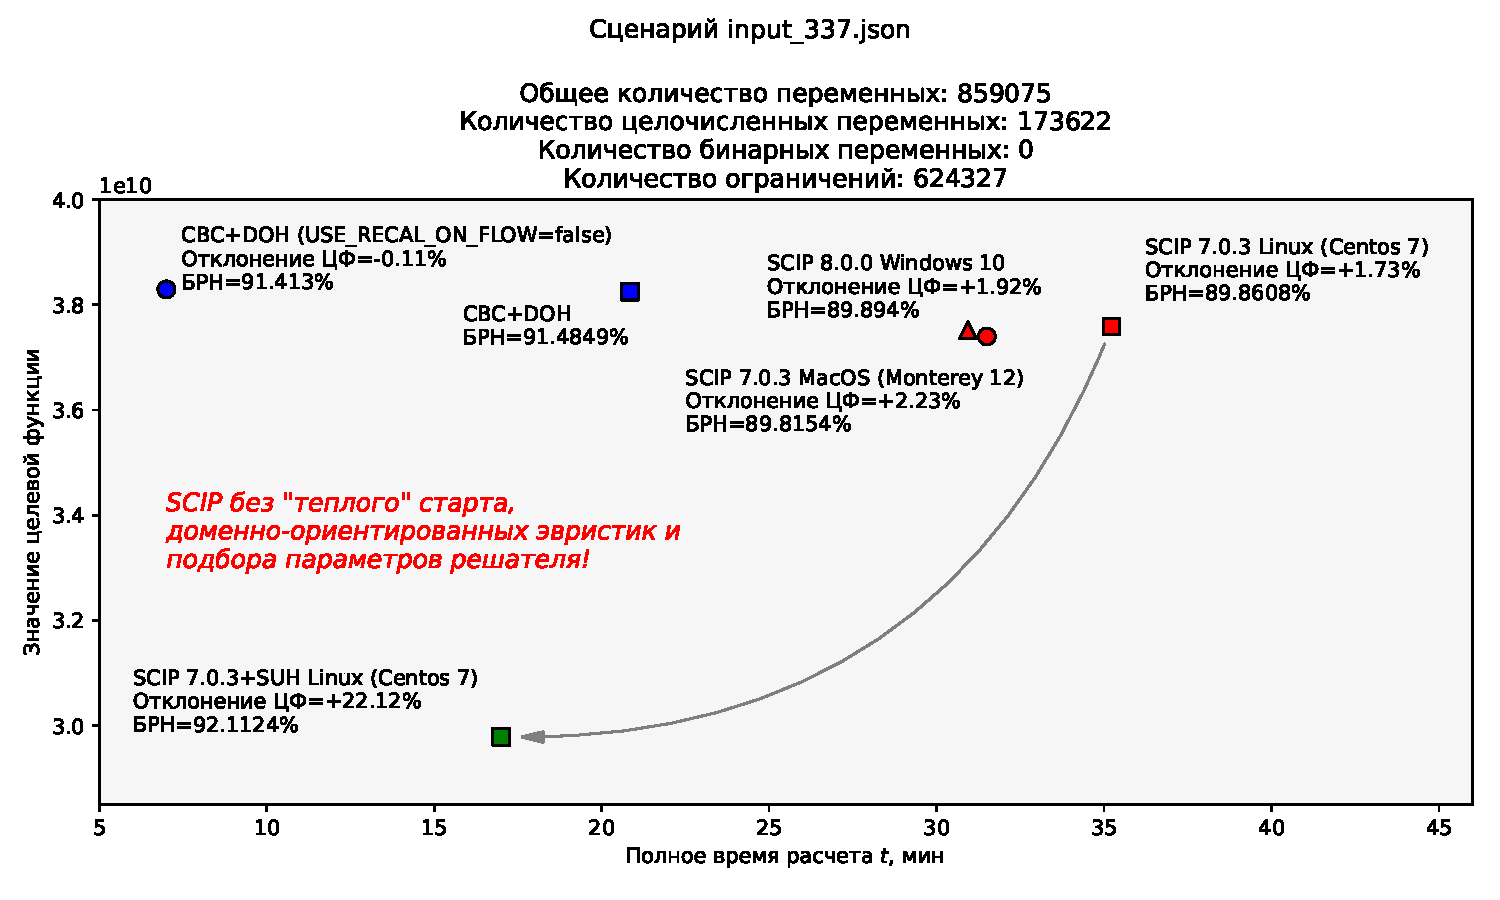
\includegraphics[scale=0.6]{figures/summary_337.pdf}
	\caption{Сводка результатов анализа эффективности метаконфигурации SUH. \\Сценарий \texttt{337} без бинарных переменных}\label{fig:summary_337}
\end{figure}

\subsubsection{Сценарий \texttt{13D686AB} без бинарных переменных}

\textbf{Статистика}\vspace*{1mm}

Общее количество переменных: 786020

Количество целочисленных переменных: 168857

Количество бинарных переменных: 0

Количество ограничений: 598414

lp-файл: \url{https://disk.yandex.ru/d/3KkYKzNl3PjGdg}

Пул решений задачи был найден с помощью следующих первичных эвристик:
\begin{itemize}
	\item INTSHIFING,
	
	\item RENS.
\end{itemize}

Файл решения задачи (метаконфигурация SUH) доступен по ссылке \url{https://disk.yandex.ru/d/EXylMeX6Ytz4tg}

Файл решения задачи (метаконфигурация FZBIVSUHPB) доступен по ссылке \url{https://disk.yandex.ru/d/dXUMVbSWRbqeDQ}

Файл статистической сводки (метаконфигурация FZBIVSUHPB) доступен по ссылке \url{https://disk.yandex.ru/d/Knavj89muxGw-w}

\vspace*{3mm}
\textbf{Вывод по сценарию}: описанная выше метаконфигурация SUH приводит к решению задачи, которое оказывается по отношению к результату на доменно-ориентированных эвристиках (\verb|USE_RECALCULATION_ON_FLOW=true|) для последнего решения из пула допустимых целочисленных решений (ОС Linux Centos 7) на 9.40\% лучше в смысле целевой функции и на 33.03\% -- в смысле временных издержек (\pic{fig:summary_13d686ab}).

Метаконфигурация FZBIVSUHPB (подробнее в разделе~\ref{sec:ikp_bins}) по отношению к тому же результату на доменно-ориентированных эвристиках дает решение задачи, которое на 10.44\% лучше в смысле целевой функции и на  75.82\% -- в смысле временных издержек (\tblref{tab:13d686ab_wo_bins}).

Синим цветом обозначен выигрыш в процентах.

{
	%\rowcolors{2}{white}{lightgray!15}
	\begin{table}[!h]
		\centering
		\caption{Сводка результатов анализа эффективности \\метаконфигураций SUH и FZBIVSUHPB. Сценарий \texttt{13d686ab} без бинарных переменных}
		\begin{tabular}{ p{2.5cm} p{3.3cm} p{3.4cm} }
			\emph{Способ} & \emph{Полное время расчета, мин} & \emph{Верхняя граница решения, $ \times 10^{9} $} \\
			\hline\hline\\[-3.5mm]
			{CBC+DOH} & 28.82 & $ 8.774743 $ \\
			\hline
			SCIP+SUH & 19.30 {\color{blue} $\ +33.03 $\%} & $ 7.949568 $ {\color{blue} $\ +9.403 $\%} \\
			\hline
			SCIP+FZB... & 6.97 {\color{blue} $\ +75.82 $\%} & $ 7.858548 $ {\color{blue} $\ +10.441 $\%} \\
		\end{tabular}\label{tab:13d686ab_wo_bins}
	\end{table}
}

\begin{figure}[!h]
	\centering
	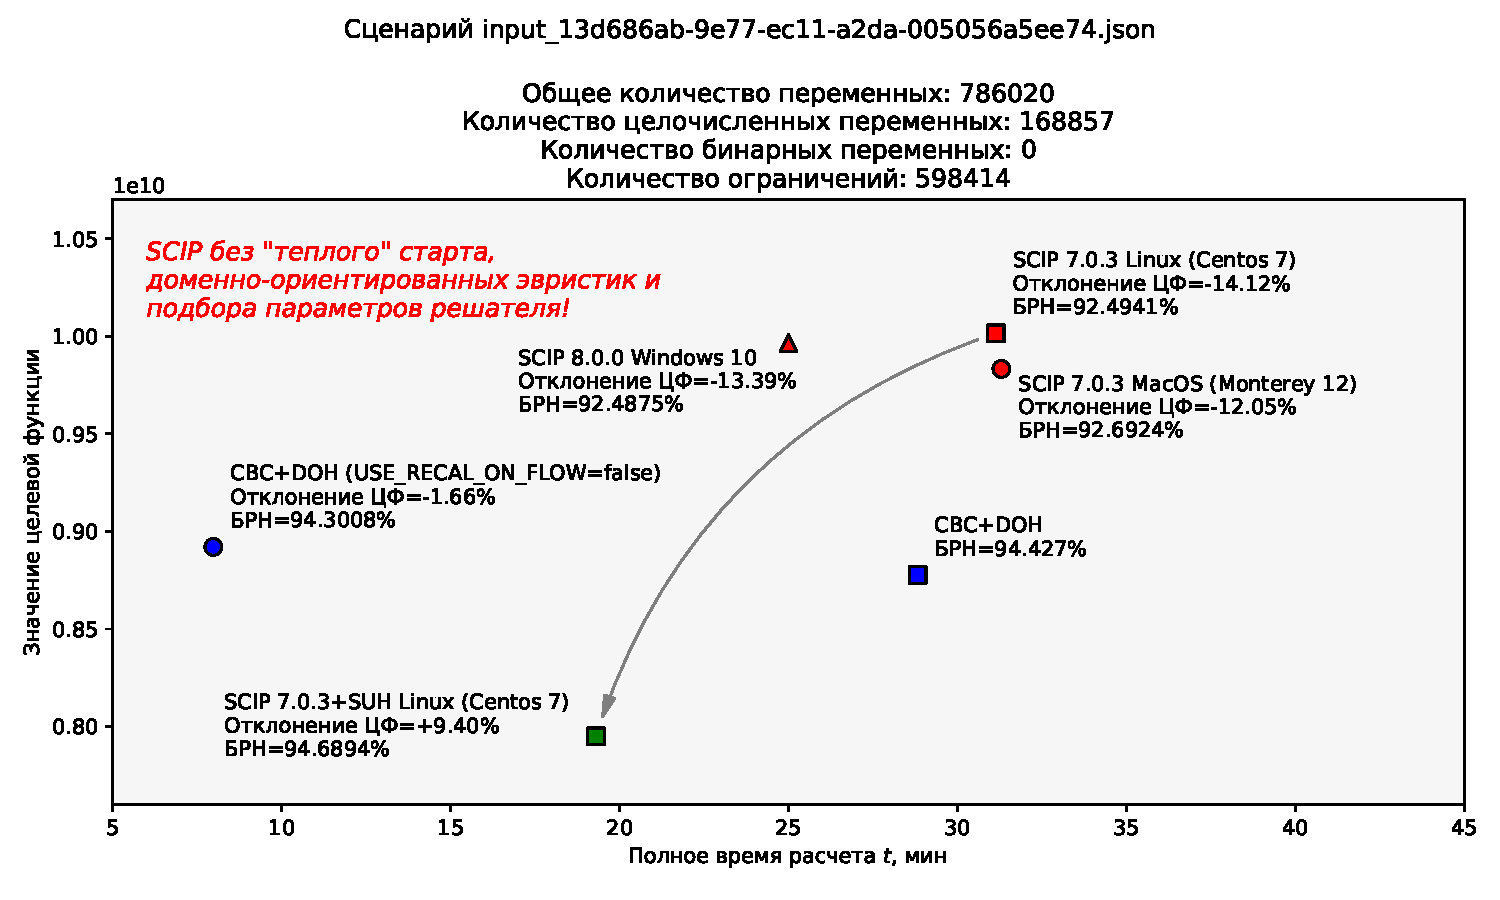
\includegraphics[scale=0.6]{figures/summary_13d686ab.pdf}
	\caption{Сводка результатов анализа эффективности метаконфигурации SUH. \\Сценарий \texttt{13d686ab} без бинарных переменных}\label{fig:summary_13d686ab}
\end{figure}

\subsubsection{Сценарий \texttt{A78CBEAD} без бинарных переменных}

\textbf{Статистика}\vspace*{1mm}

Общее количество переменных: 795400

Количество целочисленных переменных: 180160

Количество бинарных переменных: 0

Количество ограничений: 658339

lp-файл: \url{https://disk.yandex.ru/d/vTPPa1H3VFD7tA}

Пул решений задачи был найден с помощью следующих первичных эвристик:
\begin{itemize}
	\item INTSHIFING,
	
	\item RENS.
\end{itemize}

Файл решения задачи (метаконфигурация SUH) доступен по ссылке \url{https://disk.yandex.ru/d/fARVcHb66ToHxQ}

Файл решения задачи (метаконфигурация FZBIVSUHPB) доступен по ссылке \url{https://disk.yandex.ru/d/4DItEZTja77cog}

Файл статистической сводки (метаконфигурация FZBIVSUHPB) доступен по ссылке \url{https://disk.yandex.ru/d/vn1K834mY5MEng}

\vspace*{3mm}
\textbf{Вывод по сценарию}: описанная выше метаконфигурация SUH приводит к решению задачи, которое оказывается по отношению к приему на доменно-ориентированных эвристиках (\verb|USE_RECALCULATION_ON_FLOW=true|) для последнего решения из пула допустимых целочисленных решений (ОС Linux Centos 7) на 1.57\% лучше в смысле целевой функции и на 23.30\% -- в смысле временных издержек (\pic{fig:summary_a78cbead}).

Метаконфигурация FZBIVSUHPB (подробнее в разделе~\ref{sec:ikp_bins}) по отношению к приему построения решения на доменно-ориентированных эвристиках дает решение задачи, которое на 1.39\% лучше в смысле целевой функции и на  81.04\% -- в смысле временных издержек (\tblref{tab:a78cbead_wo_bins}).

Синим цветом обозначен выигрыш в процентах.

{
	%\rowcolors{2}{white}{lightgray!15}
	\begin{table}[!h]
		\centering
		\caption{Сводка результатов анализа эффективности \\метаконфигураций SUH и FZBIVSUHPB. Сценарий \texttt{a78cbead} без бинарных переменных}
		\begin{tabular}{ p{2.5cm} p{3.3cm} p{3.4cm} }
			\emph{Способ} & \emph{Полное время расчета, мин} & \emph{Верхняя граница решения, $ \times 10^{10} $} \\
			\hline\hline\\[-3.5mm]
			{CBC+DOH} & 26.05& $ 3.801546 $ \\
			\hline
			SCIP+SUH & 19.98 {\color{blue} $\ +23.30 $\%} & $ 3.741685 $ {\color{blue} $\ +1.576 $\%} \\
			\hline
			SCIP+FZB... & 4.94 {\color{blue} $\ +81.04 $\%} & $ 3.748890 $ {\color{blue} $\ +1.386 $\%} \\
		\end{tabular}\label{tab:a78cbead_wo_bins}
	\end{table}
}

\begin{figure}[!h]
	\centering
	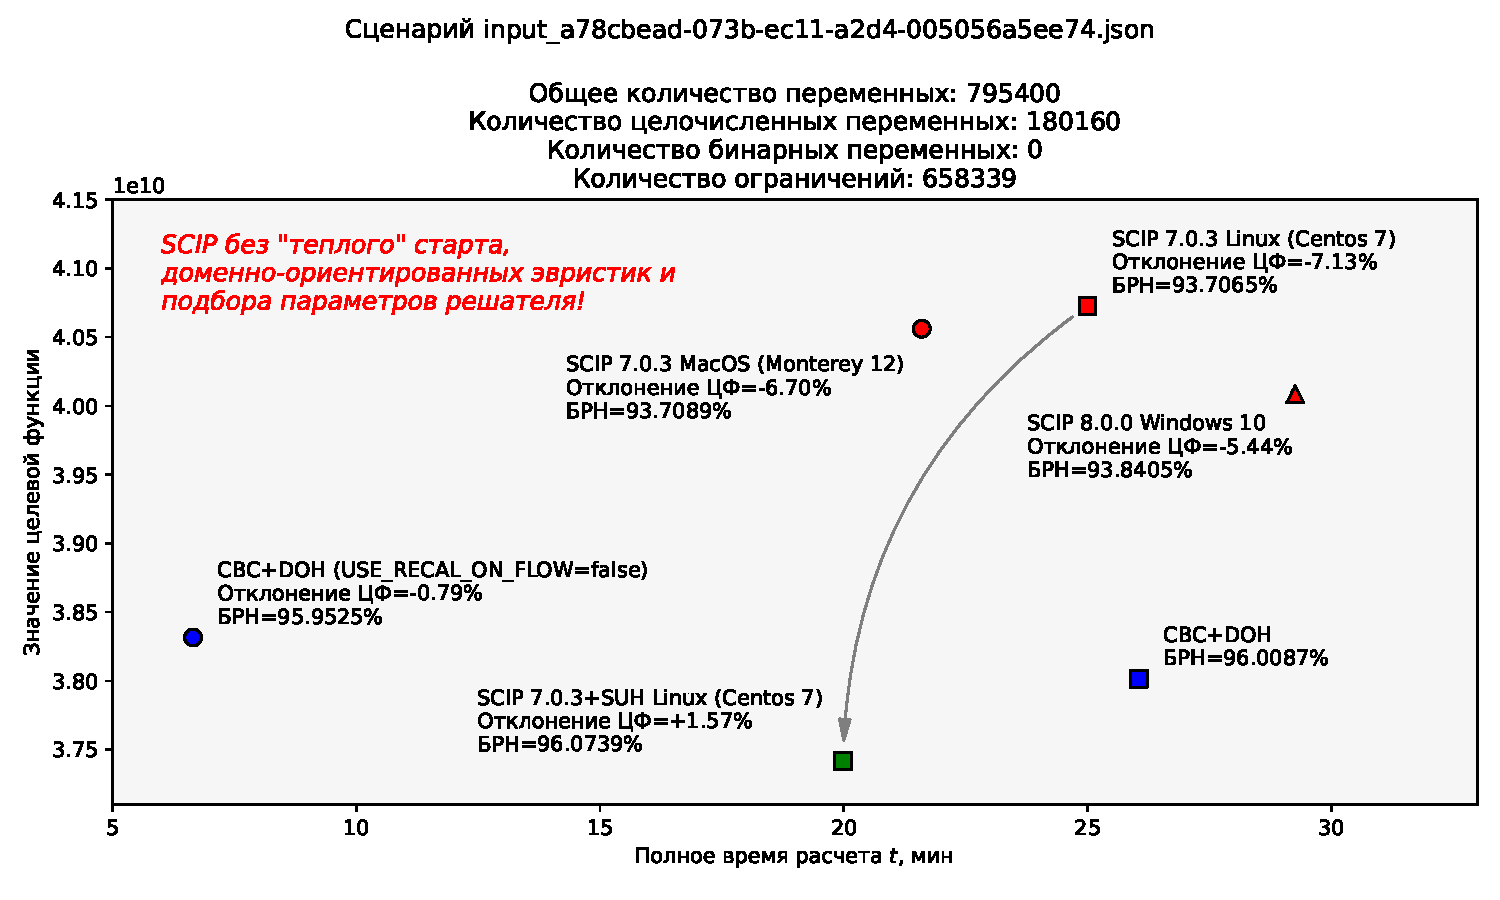
\includegraphics[scale=0.6]{figures/summary_a78cbead.pdf}
	\caption{Сводка результатов анализа эффективности метаконфигурации SUH. \\Сценарий \texttt{a78cbead} без бинарных переменных}\label{fig:summary_a78cbead}
\end{figure}

\subsubsection{Сценарий \texttt{496} (hard) без бинарных переменных}

\textbf{Статистика}\footnote{В первых скобках указана размерность задачи после шага пресолвинга с фиксацией FZBIVSUHPB, а во вторых -- с фиксацией, полученной с помощью ансамбля детекторов аномалий без подбора гиперпараметров детекторов}\vspace*{1mm}

Общее количество переменных: 864743 (48862) (90762)

Количество целочисленных переменных: 177365 (5008) (25872)

Количество бинарных переменных: 0 (332) (27)

Количество ограничений: 610819 (25438) (39119)

lp-файл: \url{https://disk.yandex.ru/d/CUA7wSn35k7Gbw}

Решение задачи было найдено с помощью первичной эвристики {INTSHIFTING}.

Файл решения задачи (метаконфигурация FZBIVSUHPB) доступен по ссылке \url{https://disk.yandex.ru/d/tbMiAbYmaAOrhg}

Файл статистической сводки (метаконфигурация FZBIVSUHPB) доступен по ссылке \url{https://disk.yandex.ru/d/AQptE3s3NF4bug}

Файл решения задачи (ансамбль детекторов аномалий) доступен по ссылке \url{https://disk.yandex.ru/d/VMZLFWoT8OftXA}

Файл статистической сводки (ансамбль детекторов аномалий) доступен по ссылке \url{https://disk.yandex.ru/d/KckqXgoKfv2fyQ}

Решение SCIP+ML получено с помощью ансамбля детекторов аномалий без подбора гиперпараметров детекторов.

\vspace*{3mm}
\textbf{Вывод по сценарию}: метаконфигурация FZBIVSUHPB (подробнее в разделе~\ref{sec:ikp_bins}) по отношению к приему на доменно-ориентированных эвристиках CBC+MS (measure of similarity) дает решение задачи, которое на 9.823\% лучше в смысле целевой функции и на  69.13\% -- в смысле временных издержек (\tblref{tab:496_wo_bins}).

Решение, полученное с помощью ансамбля детекторов аномалий, обученного на сценарии \texttt{f398266b\_bin.lp}, на 9.678\% превосходит CBC+MS в смысле целевой функции и на 71.82\% -- в смысле временных издержек.

SCIP+ML(0.10)f -- решение, полученное с помощью ансамбля детекторов аномалий без подбора параметра контаменации при первом запуске приложения, SCIP+ML(0.10)e -- то же самое, при запуске приложения в <<исследовательском режиме>> (матрица ограничений обучающего поднабора данных и релаксированные решения не вычисляются повторно).

Синим цветом обозначен выигрыш в процентах.

{
	%\rowcolors{2}{white}{lightgray!15}
	\begin{table}[!h]
		\centering
		\caption{Сводка результатов анализа эффективности \\метаконфигураций FZBIVSUHPB и ансамбля детекторов аномалий. \\Сценарий \texttt{496} без бинарных переменных}
		\begin{tabular}{ p{2.7cm} p{3.3cm} p{3.4cm} }
			\emph{Способ} & \emph{Полное время расчета, мин} & \emph{Верхняя граница решения, $ \times 10^{7} $} \\
			\hline\hline\\[-3.5mm]
			{CBC+MS}* & 5.00 & $ 6.536728 $ \\
			\hline
			Gurobi 9.12 & 5.22 {\color{red} $ \ - 0.04\% $} & 5.834197 {\color{blue} $ \ +10.747\% $}\\
			\hline
			SCIP 7.0.3d** & 15.42 {\color{red} $\ -66.15 $\%} & $ 10.66377 $ {\color{red} $\ -38.702 $\%} \\
			\hline
			SCIP+FZB... & 1.54 {\color{blue} $\ +69.13 $\%} & $ 5.894658 $ {\color{blue} $\ +9.823 $\%} \\
			\hline
			SCIP+ML(0.10)f & 4.56 {\color{blue} $\ +8.8 $\%} & 5.904120 {\color{blue} $\ +9.678 $\%} \\
			\hline
			SCIP+ML(0.10)e & 1.51 {\color{blue} $\ +69.76 $\%} & 5.904120 {\color{blue} $\ +9.678 $\%} 
		\end{tabular}\label{tab:496_wo_bins}
	\end{table}
\vspace*{-5mm}\hspace{30mm}\small{* -- опорное решение}
\hspace{15mm}\small{** -- решение было прервано}
}


\subsubsection{Сценарий \texttt{514} (hard) без бинарных переменных}

\textbf{Статистика}\footnote{В первых скобках указана размерность задачи после шага пресолвинга с фиксацией FZBIVSUHPB, а во вторых -- с фиксацией, полученной с помощью ансамбля детекторов аномалий без подбора гиперпараметров детекторов}\vspace*{1mm}

Общее количество переменных: 775879 (77367) (120764)

Количество целочисленных переменных: 145292 (5817) (32895)

Количество бинарных переменных: 0 (30) (14)

Количество ограничений: 541040 (45892) (61074)

lp-файл: \url{https://disk.yandex.ru/d/jQqSqBKb6iG-vw}

Пул решений задачи был найден с помощью следующих первичных эвристик:
\begin{itemize}
	\item INTSHIFTING,
	
	\item RENS.
\end{itemize}

Файл решения задачи (метаконфигурация FZBIVSUHPB) доступен по ссылке \url{https://disk.yandex.ru/d/lN2FdsqwEQcVTQ}

Файл статистической сводки (метаконфигурация FZBIVSUHPB) доступен по ссылке \url{https://disk.yandex.ru/d/iIdbACgh59EpVg}

Файл решения задачи (ансамбль детекторов аномалий) доступен по ссылке \url{https://disk.yandex.ru/d/5kRyOUsIOatHsQ}

Файл статистической сводки (ансамбль детекторов аномалий) доступен по ссылке \url{https://disk.yandex.ru/d/rNUU8HmeBGLFRQ}

Решение SCIP+ML получено с помощью ансамбля детекторов аномалий без подбора гиперпараметров детекторов.

\vspace*{3mm}
\textbf{Вывод по сценарию}: метаконфигурация FZBIVSUHPB (подробнее в разделе~\ref{sec:ikp_bins}) по отношению к приему построения решения с помощью меры подобия CBC+MS (measure of similarity) дает решение задачи, которое на 18.616\% лучше в смысле целевой функции и на  51.82\% хуже в смысле временных издержек (\tblref{tab:514_wo_bins}).

Решение, полученное с помощью ансамбля детекторов аномалий\footnote{Решение принудительно останавливалось на 350 секунде (параметр \texttt{limits/softtime = 350})}, обученного на сценарии \texttt{f398266b\_bin.lp}, на 19.562\% превосходит CBC+MS в смысле целевой функции и на 6.31\% -- в смысле временных издержек.

SCIP+ML(0.10)f -- решение, полученное с помощью ансамбля детекторов аномалий без подбора параметра контаменации при первом запуске приложения, SCIP+ML(0.10)e -- то же самое, при запуске приложения в <<исследовательском режиме>> (матрица ограничений обучающего поднабора данных и релаксированные решения не вычисляются повторно).

Синим цветом обозначен выигрыш в процентах, а красным -- проигрыш.

{
	%\rowcolors{2}{white}{lightgray!15}
	\begin{table}[!h]
		\centering
		\caption{Сводка результатов анализа эффективности \\метаконфигураций FZBIVSUHPB и ансамбля детекторов аномалий. \\Сценарий \texttt{514} без бинарных переменных}
		\begin{tabular}{ p{2.7cm} p{3.3cm} p{3.4cm} }
			\emph{Способ} & \emph{Полное время расчета, мин} & \emph{Верхняя граница решения, $ \times 10^{9} $} \\
			\hline\hline\\[-3.5mm]
			{CBC+MS}* & 13.00 & $ 5.243829 $ \\
			\hline
			Gurobi 9.12 & 11.(6) {\color{blue} $ +10.31 $} & $ 4.239092 $ {\color{blue} $\ +19.160 $\%} \\
			\hline
			SCIP 7.0.3d** & 60.32 {\color{red} $\ -79.47 $\%} & $ 47.82659 $ {\color{red} $\ -89.036 $\%} \\
			\hline
			SCIP+FZB... & 26.98 {\color{red} $\ -51.82 $\%} & $ 4.267692 $ {\color{blue} $\ +18.616 $\%} \\
			\hline
			SCIP+ML(0.10)f & 12.171 {\color{blue} $\ +6.38 $\%} & 4.217134 {\color{blue} $\ +19.580 $\%} \\
			\hline
			SCIP+ML(0.10)e & 6.53  {\color{blue} $\ +49.77 $\%} & 4.217134 {\color{blue} $\ +19.580 $\%}
		\end{tabular}\label{tab:514_wo_bins}
	\end{table}
\vspace{-5mm}\hspace{30mm}\small{* -- опорное решение}
\hspace{15mm}\small{** -- решение было прервано}
}

\subsubsection{Сценарий \texttt{519} (hard) без бинарных переменных}

\textbf{Статистика}\footnote{В скобках указана размерность задачи после шага пресолвинга с фиксацией FZBIVSUHPB}\vspace*{1mm}

Общее количество переменных: 684412 (75034)

Количество целочисленных переменных: 159200 (5424)

Количество бинарных переменных: 0 (44)

Количество ограничений: 447182 (44735)

lp-файл: \url{https://disk.yandex.ru/d/MMvnnYXK4J4Xxw}

Пул решений задачи был найден с помощью следующих первичных эвристик:
\begin{itemize}
	\item INTSHIFING,
	
	\item ONEOPT,
	
	\item VECLENDI,
	
	\item LINESEARCH,
	
	\item RENS.
\end{itemize}

%Файл решения задачи (метаконфигурация FZBIVSUHPB) доступен по ссылке \url{https://disk.yandex.ru/d/lN2FdsqwEQcVTQ}

%Файл статистической сводки (метаконфигурация FZBIVSUHPB) доступен по ссылке \url{https://disk.yandex.ru/d/iIdbACgh59EpVg}

Файл решения задачи (метаконфигурация FZBIVSUHPB) доступен по ссылке \url{https://disk.yandex.ru/d/25B3mUiRYdid3A}

Файл статистической сводки (метаконфигурация FZBIVSUHPB) доступен по ссылке \url{https://disk.yandex.ru/d/L3TyaXp56rZjCA}

Файл решения задачи (ансамбль детекторов аномалий) доступен по ссылке \url{}

Файл статистической сводки (ансамбль детекторов аномалий) доступен по ссылке \url{}

Решение SCIP+ML получено с помощью ансамбля детекторов аномалий без подбора гиперпараметров детекторов.

\vspace*{3mm}
\textbf{Вывод по сценарию}: метаконфигурация FZBIVSUHPB (подробнее в разделе~\ref{sec:ikp_bins}) по отношению к приему построения решения на доменно-ориентированных эвристиках CBC+MS (measure of similarity) дает решение задачи, которое на \% лучше в смысле целевой функции и на  \% хуже в смысле временных издержек (\tblref{tab:519_wo_bins}).

Решение, полученное с помощью отдельного детектора аномалий, обученного на сценарии \texttt{f398266b\_bin.lp}, на \% превосходит CBC+MS в смысле целевой функции и на \% -- в смысле временных издержек.

SCIP+ML(0.10)f -- решение, полученное с помощью ансамбля детекторов аномалий без подбора параметра контаменации при первом запуске приложения, SCIP+ML(0.10)e -- то же самое, при запуске приложения в <<исследовательском режиме>> (матрица ограничений обучающего поднабора данных и релаксированные решения не вычисляются повторно).

Синим цветом обозначен выигрыш в процентах, а красным -- проигрыш.

{
	%\rowcolors{2}{white}{lightgray!15}
	\begin{table}[!h]
		\centering
		\caption{Сводка результатов анализа эффективности \\метаконфигураций FZBIVSUHPB и ансамбля детекторов аномалий. \\Сценарий \texttt{519} без бинарных переменных}
		\begin{tabular}{ p{3.3cm} p{3.3cm} p{3.4cm} }
			\emph{Способ} & \emph{Полное время расчета, мин} & \emph{Верхняя граница решения, $ \times 10^{7} $} \\
			\hline\hline\\[-3.5mm]
			{CBC+MS}* & 6.00 & $ 7.719212 $ \\
			\hline
			Gurobi 9.12 & 3.48 {\color{blue} $\ +42.00 $\%} & $ 7.062839 $ {\color{blue} $\ +8.503 $\%} \\
			\hline
			SCIP 7.0.3d** & 41.92 {\color{red} $\ -91.70 $\%} & $ 31.59748 $ {\color{red} $\ +77.647 $\%} \\
			\hline
			SCIP+FZB (a) & 5.23 {\color{blue} $\ +12.83 $\%} & $ 7.901148 $ {\color{red} $\ -2.302 $\%} \\
			\hline
			SCIP+FZB (b) & 28.83 {\color{red} $\ -79.19 $\%} & $ 7.374810 $ {\color{blue} $\ +4.462 $\%} \\
			\hline
			SCIP+ML(0.10)f & 42.07 {\color{red} $\ -85.74 $ \%} & 7.014369 {\color{blue} $\ +9.130 $\%} \\
			\hline
%			SCIP+ML(0.10)e & 34.08 {\color{red} $\ -82.39 $ \%} & 7.011104 {\color{blue} $\ +9.173 $\%} \\
%			\hline
%			SCIP+ML(0.0468)f & 29.97 {\color{red} $\ -79.98 $ \%} & 7.147467 {\color{blue} $\ +7.408 $\%} \\
%			\hline
%			SCIP+ML(0.0468)e & 21.95 {\color{red} $\ -72.67 $ \%} & 7.147467 {\color{blue} $\ +7.408 $\%} \\
		\end{tabular}\label{tab:519_wo_bins}
	\end{table}
\vspace{-5mm}\hspace{30mm}\small{* -- опорное решение}
\hspace{15mm}\small{** -- решение было прервано}
}


\subsection{Поиск решения на сценариях \emph{с} бинарными переменными. \\Метаконфигурация FZBIVSUHPB}\label{sec:ikp_bins}

На ранних стадиях изучения проблемы высокоразмерных сценариев с бинарными переменными, поиск решения осуществлялся в семь шагов:
\begin{enumerate}
	\item  Подавить подгруппу первичных эвристик низкой эффективности (см. раздел ~\ref{sec:suh}),
	
	\item При разрешении конфликтов и ветвлении\footnote{К сожалению, на сценариях группы ИКП с бинарными переменными решателю SCIP не удается найти решение в корне дерева} отдавать предпочтение бинарным переменным,
	
	\item Найти релаксированное решение задачи,
	
	\item Подобрать порог бинаризации на релаксированном решении для бинарных переменных (см. раздел~\ref{sec:find_bin_thresh}),
	
	\item Зафиксировать \emph{нулевые} 0-bin и \emph{единичные} 1-bin \emph{бинарные переменные}; подать фиксацию решателю,
	
	\item В решении, найденном на предыдущей итерации, зафиксировать \emph{нулевые целочисленные} 0-int и \emph{единичные бинарные} 1-bin \emph{переменные}; полученную фиксацию подать на вход решателю,
	
	\item В решении, полученном на предыдущей итерации, зафиксировать \emph{нулевые бинарные} 0-bin и \emph{целочисленные} 0-int  \emph{переменные}; фиксацию подать на вход решателю.
\end{enumerate}

Процедура поиска оказалась чувствительной к параметру \texttt{autorestartnodes}. Графическая интерпретация результатов вычислительных экспериментов с разверткой процедуры поиска верхней границы решения во времени приведена на рис.~\ref{fig:a78cbead_autorestartnodes_1_2_phase}, \ref{fig:a78cbead_autorestartnodes_3_phase}, \ref{fig:50197df7_autorestartnodes} и \ref{fig:7fac4231_autorestartnodes}.

Позже описанную процедуру удалось упростить и свести к следующей \emph{метаконфигурации} {FZBIVSUHPB} (Fixed Zero Binary and Integer Variables, Suppress Useless Heuristics, Prefer Binary):
\begin{enumerate}
	\item Подавить подгруппу первичных эвристик низкой эффективности,
	
	\item При разрешении конфликтов и ветвлении отдавать предпочтение \emph{бинарным} переменным,
	
	\item Зафиксировать \emph{нулевые бинарные} 0-bin и \emph{нулевые целочисленные} 0-int  \emph{переменные} в релаксированном решении (см. раздел~\ref{sec:bin_int_relax_fix}).
\end{enumerate}

Конфигурация решателя SCIP для всех сценариев группы ИКП (с бинарными переменными) имеет вид
\begin{lstlisting}[
	title = {\sffamily scip.set. Сценарии группы ИКП с бинарными переменными},
	style = bash,
	numbers = none,
	]
# критерии останова и перезапуска
limits/time = 7200
limits/autorestartnodes = -1
limits/gap = 0.02  # решение останавливается при зазоре <= 2%

# управление стратегиями анализа конфликтов и ветвления
conflict/preferbinary = True
branching/preferbinary = True

# подавление подгруппы первичных эвристик низкой эффективности
heuristics/farkasdiving/freq = -1
heuristics/feaspump/freq = -1
heuristics/randrounding/freq = -1
heuristics/shiftandpropagate/freq = -1
heuristics/shifting/freq = -1
\end{lstlisting}

Все эксперименты проводились на виртуальной машине Linux (Centos 7) Intel Core™ i7 (8~CPUs), 3.6GHz, RAM 16Gb.

Сводка результатов вычислительных экспериментов доступна по ссылке \url{https://docs.google.com/document/d/1V9fZLT9cXkbVQ5BvMCwzKrAiASZ2v4-01Z68jVBZUBU/edit?usp=sharing}.

Кодовая база решения доступна по ссылке \url{https://gitdp.zyfra.com/ds_and_math_users/ml-dl-in-operations-reaseearches.git}

\subsubsection{Сценарий \texttt{A78CBEAD} с бинарными переменными}

\textbf{Статистика}\vspace*{1mm}

Общее количество переменных: 797818

Количество целочисленных переменных: 180160

Количество бинарных переменных: 2418

Количество ограничений: 663175

lp-файл: \url{https://disk.yandex.ru/d/JbT3KR5Yi1ZomQ}

\vspace*{5mm}\textbf{Анализ решения}\vspace*{1mm}

Пул решений задачи был найден с помощью следующих первичных эвристик:
\begin{itemize}
	\item DISTRIBUTIOINDIVING,
	
	\item ONEOPT,
	
	\item GINS.
\end{itemize}

Фргамент лога сессии SCIP
\begin{lstlisting}[
style = bash,
numbers = none
]
...
 time | node  | left  |LP iter|LP it/n|mem/heur|mdpt |vars |cons |rows |cuts |sepa|confs|strbr|  dualbound   | primalbound  |  gap   | compl. 
d1790s|  1881 |  1668 |  1010k| 296.9 |distribu|  93 |  50k|  43k|  43k|   0 |  1 | 385 |3585 | 3.757279e+10 | 3.894342e+10 |   3.65%|   7.70%
d1790s|  1881 |  1668 |  1010k| 296.9 |distribu|  93 |  50k|  43k|  43k|   0 |  1 | 385 |3585 | 3.757279e+10 | 3.894341e+10 |   3.65%|   7.70%
i1792s|  1882 |  1667 |  1011k| 297.0 |  oneopt|  93 |  50k|  43k|  43k|8612 |  0 | 385 |3585 | 3.757279e+10 | 3.893993e+10 |   3.64%|   7.70%
1796s|  1900 |  1687 |  1016k| 297.0 |  3669M |  93 |  50k|  43k|  43k|8644 |  1 | 387 |3585 | 3.757279e+10 | 3.893993e+10 |   3.64%|   2.82%
L1902s|  1982 |  1769 |  1090k| 313.4 |    gins|  93 |  50k|  43k|  43k|8935 |  1 | 398 |3590 | 3.757279e+10 | 3.875897e+10 |   3.16%|   2.83%
L1912s|  1982 |  1769 |  1090k| 313.4 |    gins|  93 |  50k|  43k|  43k|8935 |  1 | 398 |3590 | 3.757279e+10 | 3.864257e+10 |   2.85%|   2.83%
i1920s|  1982 |  1769 |  1099k| 316.2 |  oneopt|  93 |  50k|  43k|  43k|8935 |  1 | 398 |3590 | 3.757279e+10 | 3.864241e+10 |   2.85%|   2.83%
1954s|  2000 |  1787 |  1133k| 325.5 |  3731M |  93 |  50k|  43k|  43k|9004 |  1 | 398 |3591 | 3.757279e+10 | 3.864241e+10 |   2.85%|   2.83%
\end{lstlisting}

Файл решения задачи доступен по ссылке \url{https://disk.yandex.ru/d/6FPE-S5VupA6iw}

Файл статистической сводки доступен по ссылке \url{https://disk.yandex.ru/d/9G-v54ywEK1TJA}

\vspace*{3mm}
\textbf{Вывод по сценарию}: описанная выше метаконфигурация приводит к решению задачи, которое оказывается по отношению к результату на доменно-ориентированных эвристиках для последнего решения из пула допустимых целочисленных решений на 2.46\% лучше в смысле целевой функции и на 19.64\% -- в смысле временных издержек (\tblref{tab:a78cbead}).

В \tblref{tab:a78cbead}  через SCIP+MC~$ (a) $ обозначается решение, построенное на метаконфигурации SCIP, отвечающее \emph{первому} допустимому целочисленному решению, верхняя граница которого не превышает верхнюю границу решения на доменно-ориентированных эвристиках, а через SCIP+MC~$ (b) $ -- решение, отвечающее \emph{последнему} допустимому целочисленному решению в наборе полученных.

Синим цветом обозначен выигрыш в процентах.

{
%\rowcolors{2}{white}{lightgray!15}
\begin{table}[!h]
	\centering
	\caption{Сводка результатов анализа эффективности\\метаконфигурации FZBIVSUHPB. Сценарий \texttt{a78cbead} с бинарными переменными}
	\begin{tabular}{ p{2.5cm} p{3.3cm} p{3.4cm} }
		\emph{Способ} & \emph{Полное время расчета, мин} & \emph{Верхняя граница решения, $ \times 10^{10} $} \\
		\hline\hline\\[-3.5mm]
		{CBC+DOH} & 39.82 & $ 3.961502 $ \\
		\hline
		SCIP+MC ($ a $) & 29.83 {\color{blue} $\ +25.09 $\%} & $ 3.894342 $ {\color{blue} $\ +1.70 $\%} \\
		\hline
		SCIP+MC ($ b $) & 32.00 {\color{blue} $\ +19.64 $\%} & $ 3.864241 $ {\color{blue} $\ +2.46 $\%} \\
	\end{tabular}\label{tab:a78cbead}
\end{table}
}

\subsubsection{Сценарий \texttt{7FAC4231} с бинарными переменными}

\textbf{Статистика}\vspace*{1mm}

Общее количество переменных: 740251

Количество целочисленных переменных: 147789

Количество бинарных переменных: 2666

Количество ограничений: 545350

lp-файл: \url{https://disk.yandex.ru/d/3NbbjfLW5zhejQ}

\vspace*{5mm}\textbf{Анализ решения}\vspace*{1mm}

Пул решений задачи был найден с помощью следующих первичных эвристик:
\begin{itemize}
	\item INTSHIFTING,
	
	\item ONEOPT,
	
	\item GINS,
	
	\item CROSSOVER,
	
	\item ALNS.
\end{itemize}

Фрагмент лога сессии SCIP
\begin{lstlisting}[
style = bash,
numbers = none
]
...
 time | node  | left  |LP iter|LP it/n|mem/heur|mdpt |vars |cons |rows |cuts |sepa|confs|strbr|  dualbound   | primalbound  |  gap   | compl. 
r 454s|   372 |   341 | 91171 | 102.3 |intshift| 309 |  41k|  33k|  34k|2788 |  5 |  57 |3711 | 1.053077e+10 | 1.309195e+10 |  24.32%|   0.78%
i 454s|   373 |   340 | 91171 | 102.0 |  oneopt| 309 |  41k|  33k|  34k|2788 |  0 |  57 |3711 | 1.053077e+10 | 1.308634e+10 |  24.27%|   0.78%
463s|   400 |   369 | 93623 | 101.3 |  2493M | 309 |  41k|  33k|  34k|2950 |  1 |  57 |3761 | 1.053077e+10 | 1.308634e+10 |  24.27%|   0.29%
L 507s|   473 |   442 |106991 | 113.9 |    gins| 309 |  41k|  33k|  34k|3084 |  1 |  57 |3813 | 1.053077e+10 | 1.297515e+10 |  23.21%|   0.29%
L 512s|   473 |   442 |106991 | 113.9 |    gins| 309 |  41k|  33k|  34k|3084 |  1 |  57 |3813 | 1.053077e+10 | 1.292548e+10 |  22.74%|   0.29%
L 522s|   473 |   442 |106991 | 113.9 |    gins| 309 |  41k|  33k|  34k|3084 |  1 |  57 |3813 | 1.053077e+10 | 1.289283e+10 |  22.43%|   0.29%
L 525s|   473 |   442 |106991 | 113.9 |    gins| 309 |  41k|  33k|  34k|3084 |  1 |  57 |3813 | 1.053077e+10 | 1.286340e+10 |  22.15%|   0.29%
i 529s|   473 |   442 |112279 | 125.1 |  oneopt| 309 |  41k|  33k|  34k|3084 |  1 |  57 |3813 | 1.053077e+10 | 1.285668e+10 |  22.09%|   0.29%
r 531s|   474 |   443 |120630 | 142.5 |intshift| 309 |  41k|  33k|  34k|3084 |  1 |  58 |3813 | 1.053077e+10 | 1.197786e+10 |  13.74%|   0.29%
i 532s|   474 |   373 |124926 | 151.6 |  oneopt| 309 |  41k|  33k|  34k|3084 |  1 |  58 |3813 | 1.053077e+10 | 1.197230e+10 |  13.69%|   0.29%
536s|   500 |   399 |126496 | 146.9 |  2579M | 309 |  41k|  33k|  34k|3181 |  1 |  58 |3822 | 1.053077e+10 | 1.197230e+10 |  13.69%|   0.29%
567s|   600 |   499 |158520 | 175.8 |  2613M | 309 |  41k|  33k|  34k|3641 |  1 |  60 |3933 | 1.053095e+10 | 1.197230e+10 |  13.69%|   0.29%
L 739s|   659 |   554 |189783 | 207.6 |    gins| 309 |  41k|  33k|  34k|4060 |  1 |  62 |3978 | 1.053095e+10 | 1.191898e+10 |  13.18%|   0.29%
i 741s|   660 |   555 |198453 | 220.4 |  oneopt| 309 |  41k|  33k|  34k|4060 |  1 |  62 |3981 | 1.053095e+10 | 1.191889e+10 |  13.18%|   0.30%
794s|   700 |   595 |236166 | 261.7 |  2689M | 309 |  41k|  33k|  34k|4418 |  1 |  62 |4010 | 1.053095e+10 | 1.191889e+10 |  13.18%|   0.32%
836s|   800 |   695 |277232 | 280.4 |  2728M | 309 |  41k|  33k|  34k|4757 |  1 |  64 |4027 | 1.053219e+10 | 1.191889e+10 |  13.17%|   0.32%
L 967s|   860 |   693 |295017 | 281.5 |crossove| 309 |  41k|  33k|  34k|5000 |  1 |  64 |4059 | 1.053219e+10 | 1.154287e+10 |   9.60%|   0.32%
i 968s|   860 |   693 |300734 | 288.1 |  oneopt| 309 |  41k|  33k|  34k|5000 |  1 |  64 |4059 | 1.053219e+10 | 1.154284e+10 |   9.60%|   0.32%
990s|   900 |   733 |312921 | 288.9 |  2793M | 309 |  41k|  33k|  34k|5288 |  1 |  64 |4139 | 1.053219e+10 | 1.154284e+10 |   9.60%|   0.33%
1042s|  1000 |   823 |346085 | 293.2 |  2816M | 309 |  41k|  33k|  34k|5725 |  1 |  65 |4281 | 1.053219e+10 | 1.154284e+10 |   9.60%|   0.33%
L1083s|  1003 |   826 |347173 | 293.4 |    alns| 309 |  41k|  33k|  34k|5747 |  2 |  65 |4284 | 1.053219e+10 | 1.153273e+10 |   9.50%|   0.33%
i1084s|  1004 |   827 |352908 | 298.8 |  oneopt| 309 |  41k|  33k|  34k|5747 |  1 |  65 |4284 | 1.053219e+10 | 1.118743e+10 |   6.22%|   0.33%
1113s|  1100 |   699 |373504 | 291.4 |  2860M | 309 |  41k|  33k|  34k|6055 |  3 |  65 |4323 | 1.053219e+10 | 1.118743e+10 |   6.22%|   0.44%
1140s|     1 |     0 |419115 |     - |  3039M |   0 |  41k|  34k|  34k|   0 |  0 |  65 |4323 | 1.053219e+10 | 1.118743e+10 |   6.22%| unknown
\end{lstlisting}

Файл решения задачи доступен по ссылке \url{https://disk.yandex.ru/d/TmA6hqFV87eGTg}

Файл статистической сводки доступен по ссылке \url{https://disk.yandex.ru/d/CsGV_oal4OTxOQ}

\vspace*{3mm}
\textbf{Вывод по сценарию}: описанная выше метаконфигурация приводит к решению задачи, которое оказывается по отношению к результату на доменно-ориентированных эвристиках для последнего решения из пула допустимых целочисленных решений на 3.38\% лучше в смысле целевой функции и на 33.07\% -- в смысле временных издержек (\tblref{tab:7fac4231}).

В \tblref{tab:7fac4231}  через SCIP+MC~$ (a) $ обозначается решение, построенное на метаконфигурации SCIP, отвечающее \emph{первому} допустимому целочисленному решению, верхняя граница которого не превышает верхнюю границу решения на доменно-ориентированных эвристиках, а через SCIP+MC~$ (b) $ -- решение, отвечающее \emph{последнему} допустимому целочисленному решению в наборе полученных.

Синим цветом обозначен выигрыш в процентах.

{
	%\rowcolors{2}{white}{lightgray!15}
	\begin{table}[!h]
		\centering
		\caption{Сводка результатов анализа эффективности\\метаконфигурации FZBIVSUHPB. Сценарий \texttt{7fac4231} с бинарными переменными}
		\begin{tabular}{ p{2.5cm} p{3.3cm} p{3.4cm} }
			\emph{Способ} & \emph{Полное время расчета, мин} & \emph{Верхняя граница решения, $ \times 10^{10} $} \\
			\hline\hline\\[-3.5mm]
			{CBC+DOH} & 27.00 & $ 1.157865 $ \\
			\hline
			SCIP+MC ($ a $) & 18.05 {\color{blue} $\ +33.15 $\%} & $ 1.153273 $ {\color{blue} $\ +0.40 $\%} \\
			\hline
			SCIP+MC ($ b $) & 18.07 {\color{blue} $\ +33.07 $\%} & $ 1.118743 $ {\color{blue} $\ +3.38 $\%} \\
		\end{tabular}\label{tab:7fac4231}
	\end{table}
}

\subsubsection{Сценарий \texttt{50197DF7} с бинарными переменными}

\textbf{Статистика}\vspace*{1mm}

Общее количество переменных: 720954

Количество целочисленных переменных: 159332

Количество бинарных переменных: 2490

Количество ограничений: 600777

lp-файл: \url{https://disk.yandex.ru/d/qWeSKb2WEs6kQA}

\vspace*{5mm}\textbf{Анализ решения}\vspace*{1mm}

Пул решений задачи был найден с помощью следующих первичных эвристик:
\begin{itemize}
	\item INTSHIFTING,
	
	\item ONEOPT,
	
	\item GINS.
\end{itemize}

Фрагмент лога сессии SCIP
\begin{lstlisting}[
	style = bash,
	numbers = none
	]
	...
 time | node  | left  |LP iter|LP it/n|mem/heur|mdpt |vars |cons |rows |cuts |sepa|confs|strbr|  dualbound   | primalbound  |  gap   | compl. 
r 836s|   963 |   948 |155676 |  53.5 |intshift| 409 |  41k|  34k|  35k|4367 |  1 |  69 |7354 | 3.554610e+10 | 3.676991e+10 |   3.44%| unknown
i 836s|   964 |   947 |155676 |  53.5 |  oneopt| 409 |  41k|  34k|  35k|4367 |  0 |  69 |7354 | 3.554610e+10 | 3.676497e+10 |   3.43%| unknown
846s|  1000 |   985 |157559 |  53.4 |  2577M | 409 |  41k|  34k|  35k|4396 |  1 |  69 |7444 | 3.554610e+10 | 3.676497e+10 |   3.43%| unknown
L 885s|  1064 |  1049 |157869 |  50.5 |    gins| 409 |  41k|  34k|  35k|4397 |  1 |  69 |7484 | 3.554610e+10 | 3.659894e+10 |   2.96%| unknown
L 931s|  1064 |  1049 |157869 |  50.5 |    gins| 409 |  41k|  34k|  35k|4397 |  1 |  69 |7484 | 3.554610e+10 | 3.656967e+10 |   2.88%| unknown
i 962s|  1064 |  1049 |161589 |  54.0 |  oneopt| 409 |  41k|  34k|  35k|4397 |  1 |  69 |7484 | 3.554610e+10 | 3.656967e+10 |   2.88%| unknown
969s|  1100 |  1085 |161769 |  52.4 |  2620M | 409 |  41k|  34k|  35k|4397 |  1 |  69 |7532 | 3.554610e+10 | 3.656967e+10 |   2.88%| unknown
L 988s|  1164 |  1149 |161992 |  49.7 |    gins| 409 |  41k|  34k|  35k|4397 |  1 |  69 |7557 | 3.554610e+10 | 3.630031e+10 |   2.12%| unknown
L 993s|  1164 |  1149 |161992 |  49.7 |    gins| 409 |  41k|  34k|  35k|4397 |  1 |  69 |7557 | 3.554610e+10 | 3.625804e+10 |   2.00%| unknown
L1000s|  1164 |  1149 |161992 |  49.7 |    gins| 409 |  41k|  34k|  35k|4397 |  1 |  69 |7557 | 3.554610e+10 | 3.623675e+10 |   1.94%| unknown
\end{lstlisting}

Файл решения задачи доступен по ссылке \url{https://disk.yandex.ru/d/2_FDqS70q0UBqA}

Файл статистической сводки доступен по ссылке \url{https://disk.yandex.ru/d/SkRLoRYzQDI-Aw}

\vspace*{3mm}
\textbf{Вывод по сценарию}: описанная выше метаконфигурация приводит к решению задачи, которое оказывается по отношению к результату на доменно-ориентированных эвристиках для последнего решения из пула допустимых целочисленных решений на 2.87\% лучше в смысле целевой функции и на 36.08\% -- в смысле временных издержек (\tblref{tab:50197df7}).

В \tblref{tab:50197df7}  через SCIP+MC~$ (a) $ обозначается решение, построенное на метаконфигурации SCIP, отвечающее \emph{первому} допустимому целочисленному решению, верхняя граница которого не превышает верхнюю границу решения на доменно-ориентированных эвристиках, а через SCIP+MC~$ (b) $ -- решение, отвечающее \emph{последнему} допустимому целочисленному решению в наборе полученных.

Синим цветом обозначен выигрыш в процентах.

{
	%\rowcolors{2}{white}{lightgray!15}
	\begin{table}[!h]
		\centering
		\caption{Сводка результатов анализа эффективности\\метаконфигурации FZBIVSUHPB. Сценарий \texttt{50197df7} с бинарными переменными}
		\begin{tabular}{ p{2.5cm} p{3.3cm} p{3.4cm} }
			\emph{Способ} & \emph{Полное время расчета, мин} & \emph{Верхняя граница решения, $ \times 10^{10} $} \\
			\hline\hline\\[-3.5mm]
			{CBC+DOH} & 28.27 & $ 3.730552 $ \\
			\hline
			SCIP+MC ($ a $) & 13.93 {\color{blue} $\ +50.73 $\%} & $ 3.676991 $ {\color{blue} $\ +1.44 $\%} \\
			\hline
			SCIP+MC ($ b $) & 18.07 {\color{blue} $\ +36.08 $\%} & $ 3.623675 $ {\color{blue} $\ +2.87 $\%} \\
		\end{tabular}\label{tab:50197df7}
	\end{table}
}

\subsubsection{Сценарий \texttt{F398266B} с бинарными переменными}\label{sec:f398266b_bin}

\textbf{Статистика}\vspace*{1mm}

Общее количество переменных: 777271

Количество целочисленных переменных: 172449

Количество бинарных переменных: 2370

Количество ограничений: 655003

lp-файл: \url{https://disk.yandex.ru/d/4YFYJSB1I1wsmQ} 

\vspace*{5mm}\textbf{Анализ решения}\vspace*{1mm}

Пул решений задачи был найден с помощью следующих первичных эвристик:
\begin{itemize}
	\item DISTRIBUTIOINDIVING,
	
	\item ONEOPT,
	
	\item CROSSOVER.
\end{itemize}

Фрагмент лога сессии SCIP
\begin{lstlisting}[
	style = bash,
	numbers = none
	]
	...
 time | node  | left  |LP iter|LP it/n|mem/heur|mdpt |vars |cons |rows |cuts |sepa|confs|strbr|  dualbound   | primalbound  |  gap   | compl. 
d1163s|   433 |   434 |462507 | 790.8 |distribu|  51 |  59k|  48k|  49k|   0 |  1 |  17 |1387 | 5.857793e+10 | 6.054807e+10 |   3.36%| unknown
d1164s|   433 |   434 |462644 | 791.1 |distribu|  51 |  59k|  48k|  49k|   0 |  1 |  17 |1387 | 5.857793e+10 | 6.054779e+10 |   3.36%| unknown
d1164s|   433 |   434 |462746 | 791.3 |distribu|  51 |  59k|  48k|  49k|   0 |  1 |  17 |1387 | 5.857793e+10 | 6.054778e+10 |   3.36%| unknown
d1164s|   433 |   434 |462780 | 791.4 |distribu|  51 |  59k|  48k|  49k|   0 |  1 |  17 |1387 | 5.857793e+10 | 6.054776e+10 |   3.36%| unknown
d1164s|   433 |   434 |462801 | 791.4 |distribu|  51 |  59k|  48k|  49k|   0 |  1 |  17 |1387 | 5.857793e+10 | 6.054776e+10 |   3.36%| unknown
d1165s|   433 |   434 |462836 | 791.5 |distribu|  51 |  59k|  48k|  49k|   0 |  1 |  17 |1387 | 5.857793e+10 | 6.054776e+10 |   3.36%| unknown
d1165s|   433 |   434 |462856 | 791.6 |distribu|  51 |  59k|  48k|  49k|   0 |  1 |  17 |1387 | 5.857793e+10 | 6.054774e+10 |   3.36%| unknown
i1167s|   434 |   433 |463020 | 790.1 |  oneopt|  51 |  59k|  48k|  49k|4333 |  0 |  17 |1387 | 5.857793e+10 | 6.053918e+10 |   3.35%| unknown
1250s|   500 |   501 |531180 | 822.2 |  3321M |  51 |  59k|  48k|  49k|4529 |  1 |  26 |1402 | 5.857793e+10 | 6.053918e+10 |   3.35%| unknown
1579s|   600 |   601 |663342 | 905.6 |  3398M |  51 |  59k|  48k|  49k|5175 |  1 |  36 |1426 | 5.857932e+10 | 6.053918e+10 |   3.35%| unknown
L1892s|   634 |   635 |704819 | 922.5 |crossove|  55 |  59k|  48k|  49k|5448 |  2 |  41 |1433 | 5.858028e+10 | 6.021605e+10 |   2.79%| unknown
i1895s|   634 |   635 |715376 | 939.1 |  oneopt|  55 |  59k|  48k|  49k|5448 |  2 |  41 |1433 | 5.858028e+10 | 6.021603e+10 |   2.79%| unknown
1952s|   700 |   701 |770566 | 929.4 |  3457M |  63 |  59k|  48k|  49k|5644 |  1 |  50 |1442 | 5.858050e+10 | 6.021603e+10 |   2.79%| unknown
2095s|   800 |   801 |879949 | 950.0 |  3489M |  65 |  59k|  48k|  49k|5964 |  1 |  62 |1476 | 5.858065e+10 | 6.021603e+10 |   2.79%| unknown
\end{lstlisting}

Файл решения задачи доступен по ссылке \url{https://disk.yandex.ru/d/KXzdrUx6TZbXEw}

Файл статистической сводки доступен по ссылке \url{https://disk.yandex.ru/d/FERoaFsr5zbkjA}

\vspace*{3mm}
\textbf{Вывод по сценарию}: описанная выше метаконфигурация приводит к решению задачи, которое оказывается по отношению к результату на доменно-ориентированных эвристиках для последнего решения из пула допустимых целочисленных решений на 0.97\% лучше в смысле целевой функции и на 56.24\% -- в смысле временных издержек (\tblref{tab:f398266b}).

В \tblref{tab:f398266b}  через SCIP+MC~$ (a) $ обозначается решение, построенное на метаконфигурации SCIP, отвечающее \emph{первому} допустимому целочисленному решению, верхняя граница которого не превышает верхнюю границу решения на доменно-ориентированных эвристиках, а через SCIP+MC~$ (b) $ -- решение, отвечающее \emph{последнему} допустимому целочисленному решению в наборе полученных.

Синим цветом обозначен выигрыш в процентах.

{
	%\rowcolors{2}{white}{lightgray!15}
	\begin{table}[!h]
		\centering
		\caption{Сводка результатов анализа эффективности\\метаконфигурации FZBIVSUHPB. Сценарий \texttt{f398266b} с бинарными переменными}
		\begin{tabular}{ p{2.5cm} p{3.3cm} p{3.4cm} }
			\emph{Способ} & \emph{Полное время расчета, мин} & \emph{Верхняя граница решения, $ \times 10^{10} $} \\
			\hline\hline\\[-3.5mm]
			{CBC+DOH} & 72.17 & $ 6.080841 $ \\
			\hline
			SCIP+MC ($ a $) & 19.38 {\color{blue} $\ +73.15 $\%} & $ 6.054807 $ {\color{blue} $\ +0.43 $\%} \\
			\hline
			SCIP+MC ($ b $) & 31.58 {\color{blue} $\ +56.24 $\%} & $ 6.021603 $ {\color{blue} $\ +0.97 $\%} \\
		\end{tabular}\label{tab:f398266b}
	\end{table}
}

\subsubsection{Сценарий \texttt{337} с бинарными переменными}

\textbf{Статистика}\vspace*{1mm}

Общее количество переменных: 859230

Количество целочисленных переменных: 173622

Количество бинарных переменных: 155

Количество ограничений: 624637

lp-файл: \url{https://disk.yandex.ru/d/Kc11p9v7D-kxYA}

\vspace*{5mm}\textbf{Анализ решения}\vspace*{1mm}

Пул решений задачи был найден с помощью следующих первичных эвристик:
\begin{itemize}
	\item INTSHIFTING,
	
	\item RENS,
	
	\item ONEOPT.
\end{itemize}

Фрагмент лога сессии SCIP

\begin{lstlisting}[
style = bash,
numbers = none
]
time | node  | left  |LP iter|LP it/n|mem/heur|mdpt |vars |cons |rows |cuts |sepa|confs|strbr|  dualbound   | primalbound  |  gap   | compl. 
r 107s|     1 |     0 | 55407 |     - |intshift|   0 |  56k|  43k|  45k|1799 | 13 |   0 |   0 | 2.947544e+10 | 4.344720e+10 |  47.40%| unknown
L 247s|     1 |     0 | 55407 |     - |    rens|   0 |  56k|  43k|  45k|1799 | 13 |   0 |   0 | 2.947544e+10 | 3.022206e+10 |   2.53%| unknown
249s|     1 |     0 | 55407 |     - |  2785M |   0 |  56k|  43k|  45k|1799 | 13 |   0 |   0 | 2.947544e+10 | 3.022206e+10 |   2.53%| unknown
i 250s|     1 |     0 | 58839 |     - |  oneopt|   0 |  56k|  43k|  45k|1799 | 13 |   0 |   0 | 2.947544e+10 | 3.022205e+10 |   2.53%| unknown
250s|     1 |     0 | 58839 |     - |  2809M |   0 |  56k|  43k|  45k|1799 | 13 |   0 |   0 | 2.947544e+10 | 3.022205e+10 |   2.53%| unknown
251s|     1 |     0 | 58891 |     - |  2813M |   0 |  56k|  43k|  45k|1820 | 14 |   0 |   0 | 2.947544e+10 | 3.022205e+10 |   2.53%| unknown
251s|     1 |     0 | 58900 |     - |  2813M |   0 |  56k|  43k|  44k|1824 | 15 |   0 |   0 | 2.947544e+10 | 3.022205e+10 |   2.53%| unknown
253s|     1 |     0 | 59074 |     - |  2816M |   0 |  56k|  43k|  44k|1824 | 15 |   0 |  12 | 2.947544e+10 | 3.022205e+10 |   2.53%| unknown
254s|     1 |     0 | 59236 |     - |  2821M |   0 |  56k|  43k|  44k|1918 | 16 |   0 |  12 | 2.948327e+10 | 3.022205e+10 |   2.51%| unknown
254s|     1 |     0 | 59300 |     - |  2821M |   0 |  56k|  43k|  44k|1945 | 17 |   0 |  12 | 2.948327e+10 | 3.022205e+10 |   2.51%| unknown
255s|     1 |     0 | 59321 |     - |  2821M |   0 |  56k|  43k|  44k|1945 | 17 |   0 |  19 | 2.948327e+10 | 3.022205e+10 |   2.51%| unknown
256s|     1 |     0 | 59349 |     - |  2825M |   0 |  56k|  43k|  44k|1959 | 18 |   0 |  19 | 2.948327e+10 | 3.022205e+10 |   2.51%| unknown
256s|     1 |     0 | 59352 |     - |  2825M |   0 |  56k|  43k|  44k|1964 | 19 |   0 |  19 | 2.948327e+10 | 3.022205e+10 |   2.51%| unknown
258s|     1 |     0 | 59368 |     - |  2825M |   0 |  56k|  43k|  44k|1964 | 19 |   0 |  35 | 2.957927e+10 | 3.022205e+10 |   2.17%| unknown
259s|     1 |     0 | 59451 |     - |  2829M |   0 |  56k|  43k|  44k|2014 | 20 |   0 |  35 | 2.957927e+10 | 3.022205e+10 |   2.17%| unknown
259s|     1 |     0 | 59466 |     - |  2829M |   0 |  56k|  43k|  44k|2024 | 21 |   0 |  35 | 2.957927e+10 | 3.022205e+10 |   2.17%| unknown
259s|     1 |     2 | 59466 |     - |  2829M |   0 |  56k|  43k|  44k|2024 | 21 |   0 |  35 | 2.957927e+10 | 3.022205e+10 |   2.17%| unknown
\end{lstlisting}

Файл решения задачи доступен по ссылке \url{https://disk.yandex.ru/d/zwVhKYKEMlMlQw}

Файл статистической сводки доступен по ссылке \url{https://disk.yandex.ru/d/T9sAbRH6uWh4Uw}

\vspace*{3mm}
\textbf{Вывод по сценарию}: описанная выше метаконфигурация приводит к решению задачи, которое оказывается по отношению к результату на доменно-ориентированных эвристиках для последнего решения из пула допустимых целочисленных решений на ...\% лучше в смысле целевой функции и на ...\% -- в смысле временных издержек (\tblref{tab:337}).

В \tblref{tab:337}  через SCIP+MC~$ (a) $ обозначается решение, построенное на метаконфигурации SCIP, отвечающее \emph{первому} допустимому целочисленному решению, верхняя граница которого не превышает верхнюю границу решения на доменно-ориентированных эвристиках, а через SCIP+MC~$ (b) $ -- решение, отвечающее \emph{последнему} допустимому целочисленному решению в наборе полученных.

Синим цветом обозначен выигрыш в процентах.

{
	%\rowcolors{2}{white}{lightgray!15}
	\begin{table}[!h]
		\centering
		\caption{Сводка результатов анализа эффективности\\метаконфигурации FZBIVSUHPB. Сценарий \texttt{337} с бинарными переменными}
		\begin{tabular}{ p{2.5cm} p{3.3cm} p{3.4cm} }
			\emph{Способ} & \emph{Полное время расчета, мин} & \emph{Верхняя граница решения, $ \times 10^{10} $} \\
			\hline\hline\\[-3.5mm]
			{CBC+DOH} & 18.00 & $ 4.047865 $ \\
			\hline
			SCIP+MC ($ a $) & 4.12 {\color{blue} $\ +77.11 $\%} & $ 3.022206 $ {\color{blue} $\ +25.34 $\%} \\
			\hline
			SCIP+MC ($ b $) &  4.30 {\color{blue} $\ +76.11 $\%} & $ 3.022205 $ {\color{blue} $\ +25.34 $\%} \\
		\end{tabular}\label{tab:337}
	\end{table}







%\begin{landscape}
	\begin{figure}[!h]
		\centering
		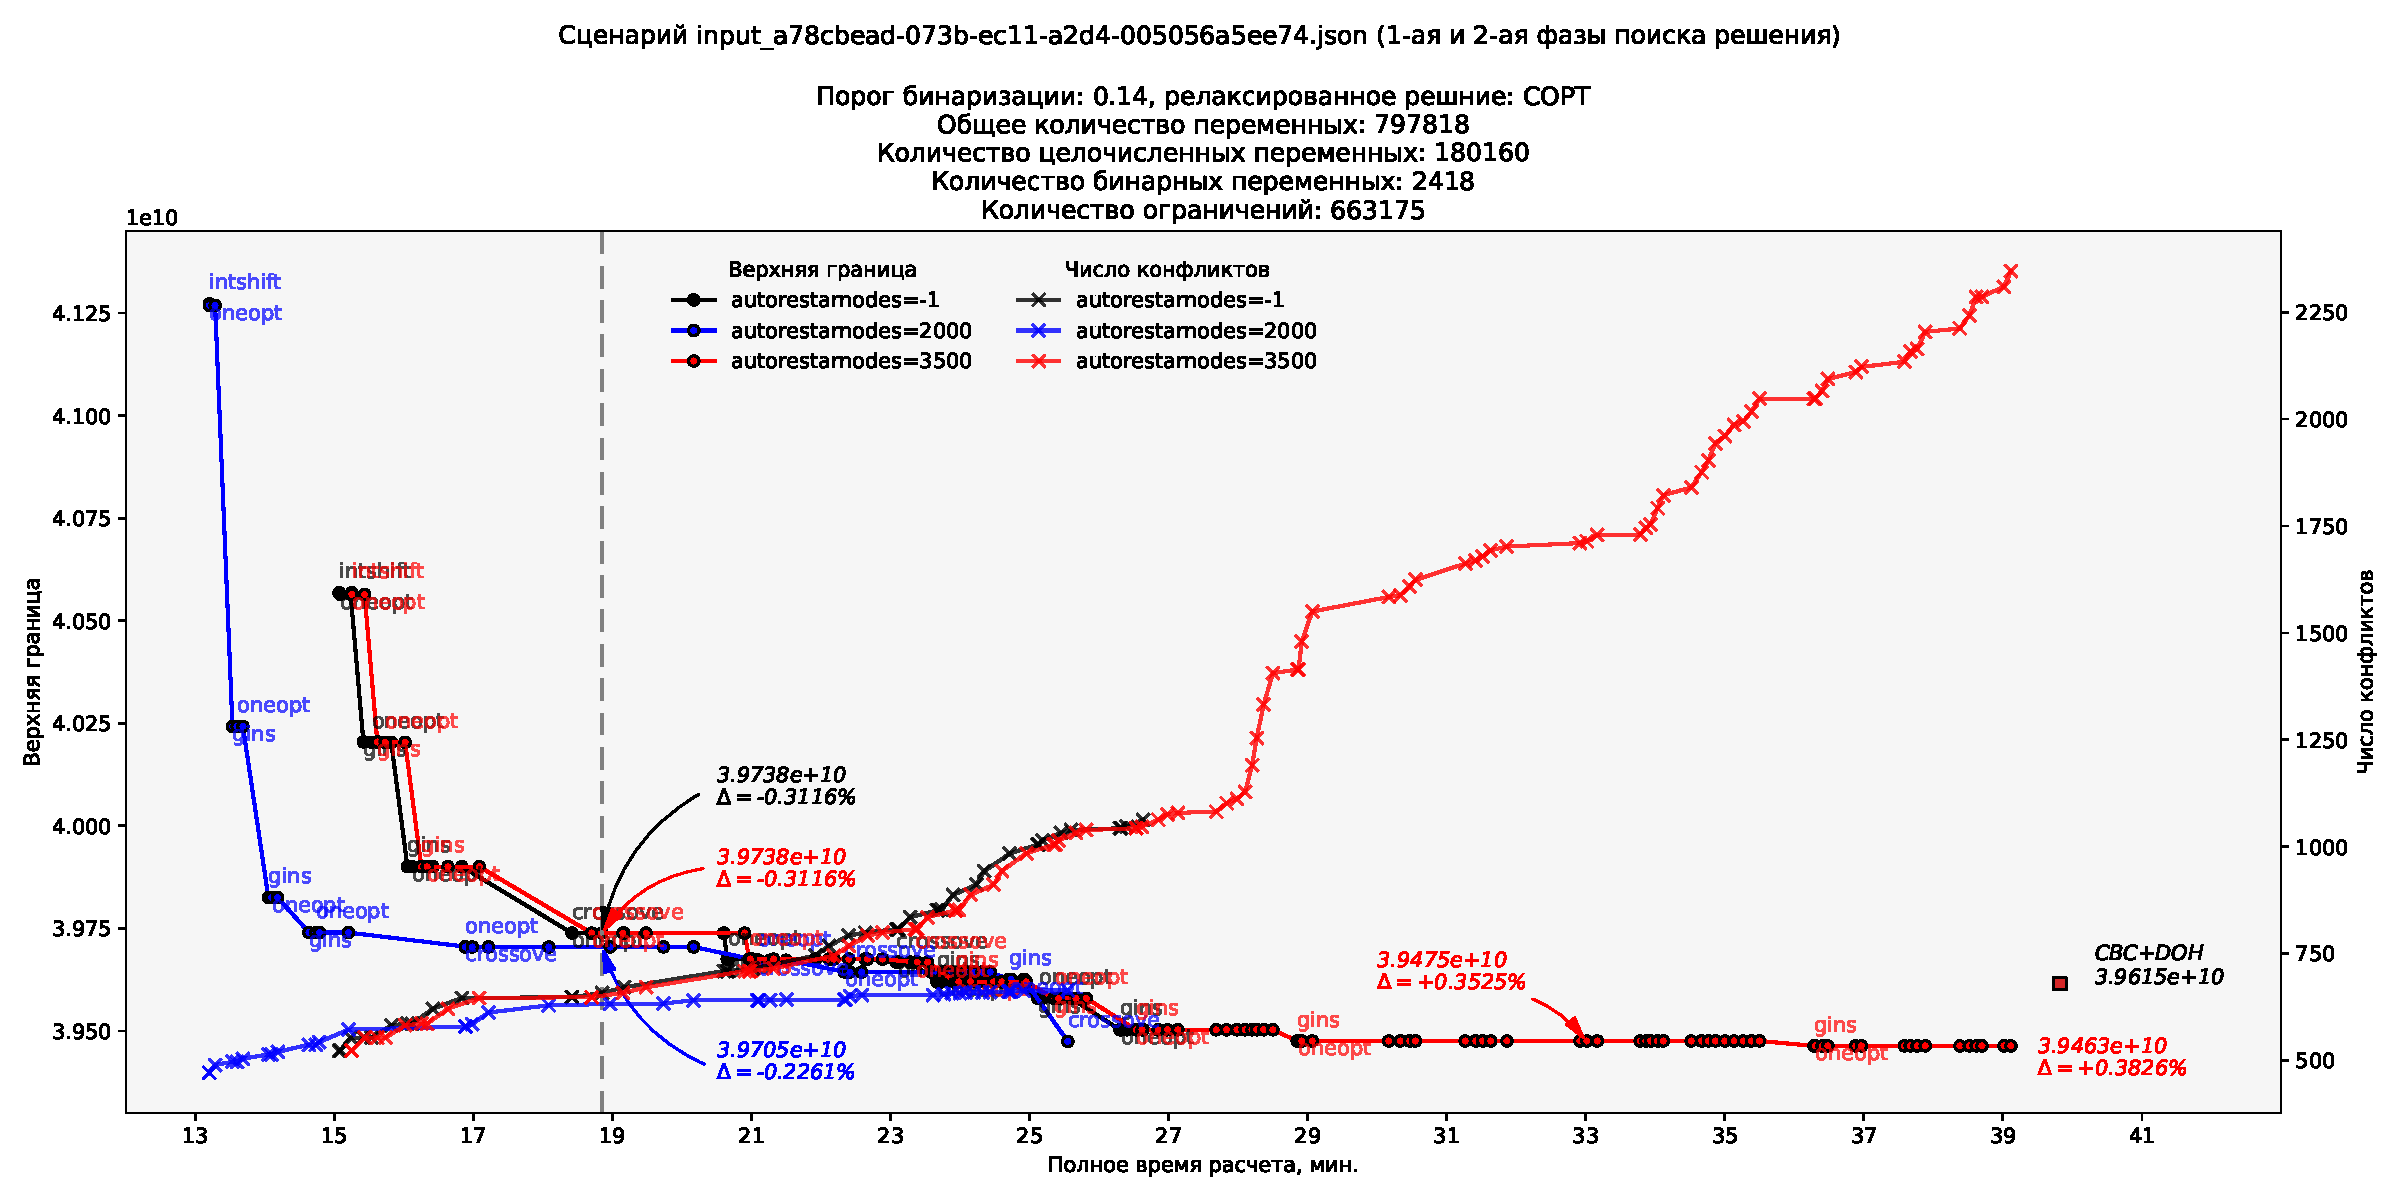
\includegraphics[scale=0.42]{figures/a78cbead_autorestartnodes_1_2_phase.pdf}
		\caption{ Динамика изменения верхней границы решения и числа конфликтов во времени в зависимости \\от значения параметра \texttt{autorestartnodes}. Сценарий \texttt{input\_a78cbead}. Первая и вторая фазы поиска решения }\label{fig:a78cbead_autorestartnodes_1_2_phase}
	\end{figure}
%\end{landscape}

%\begin{landscape}
\begin{figure}[!h]
	\centering
	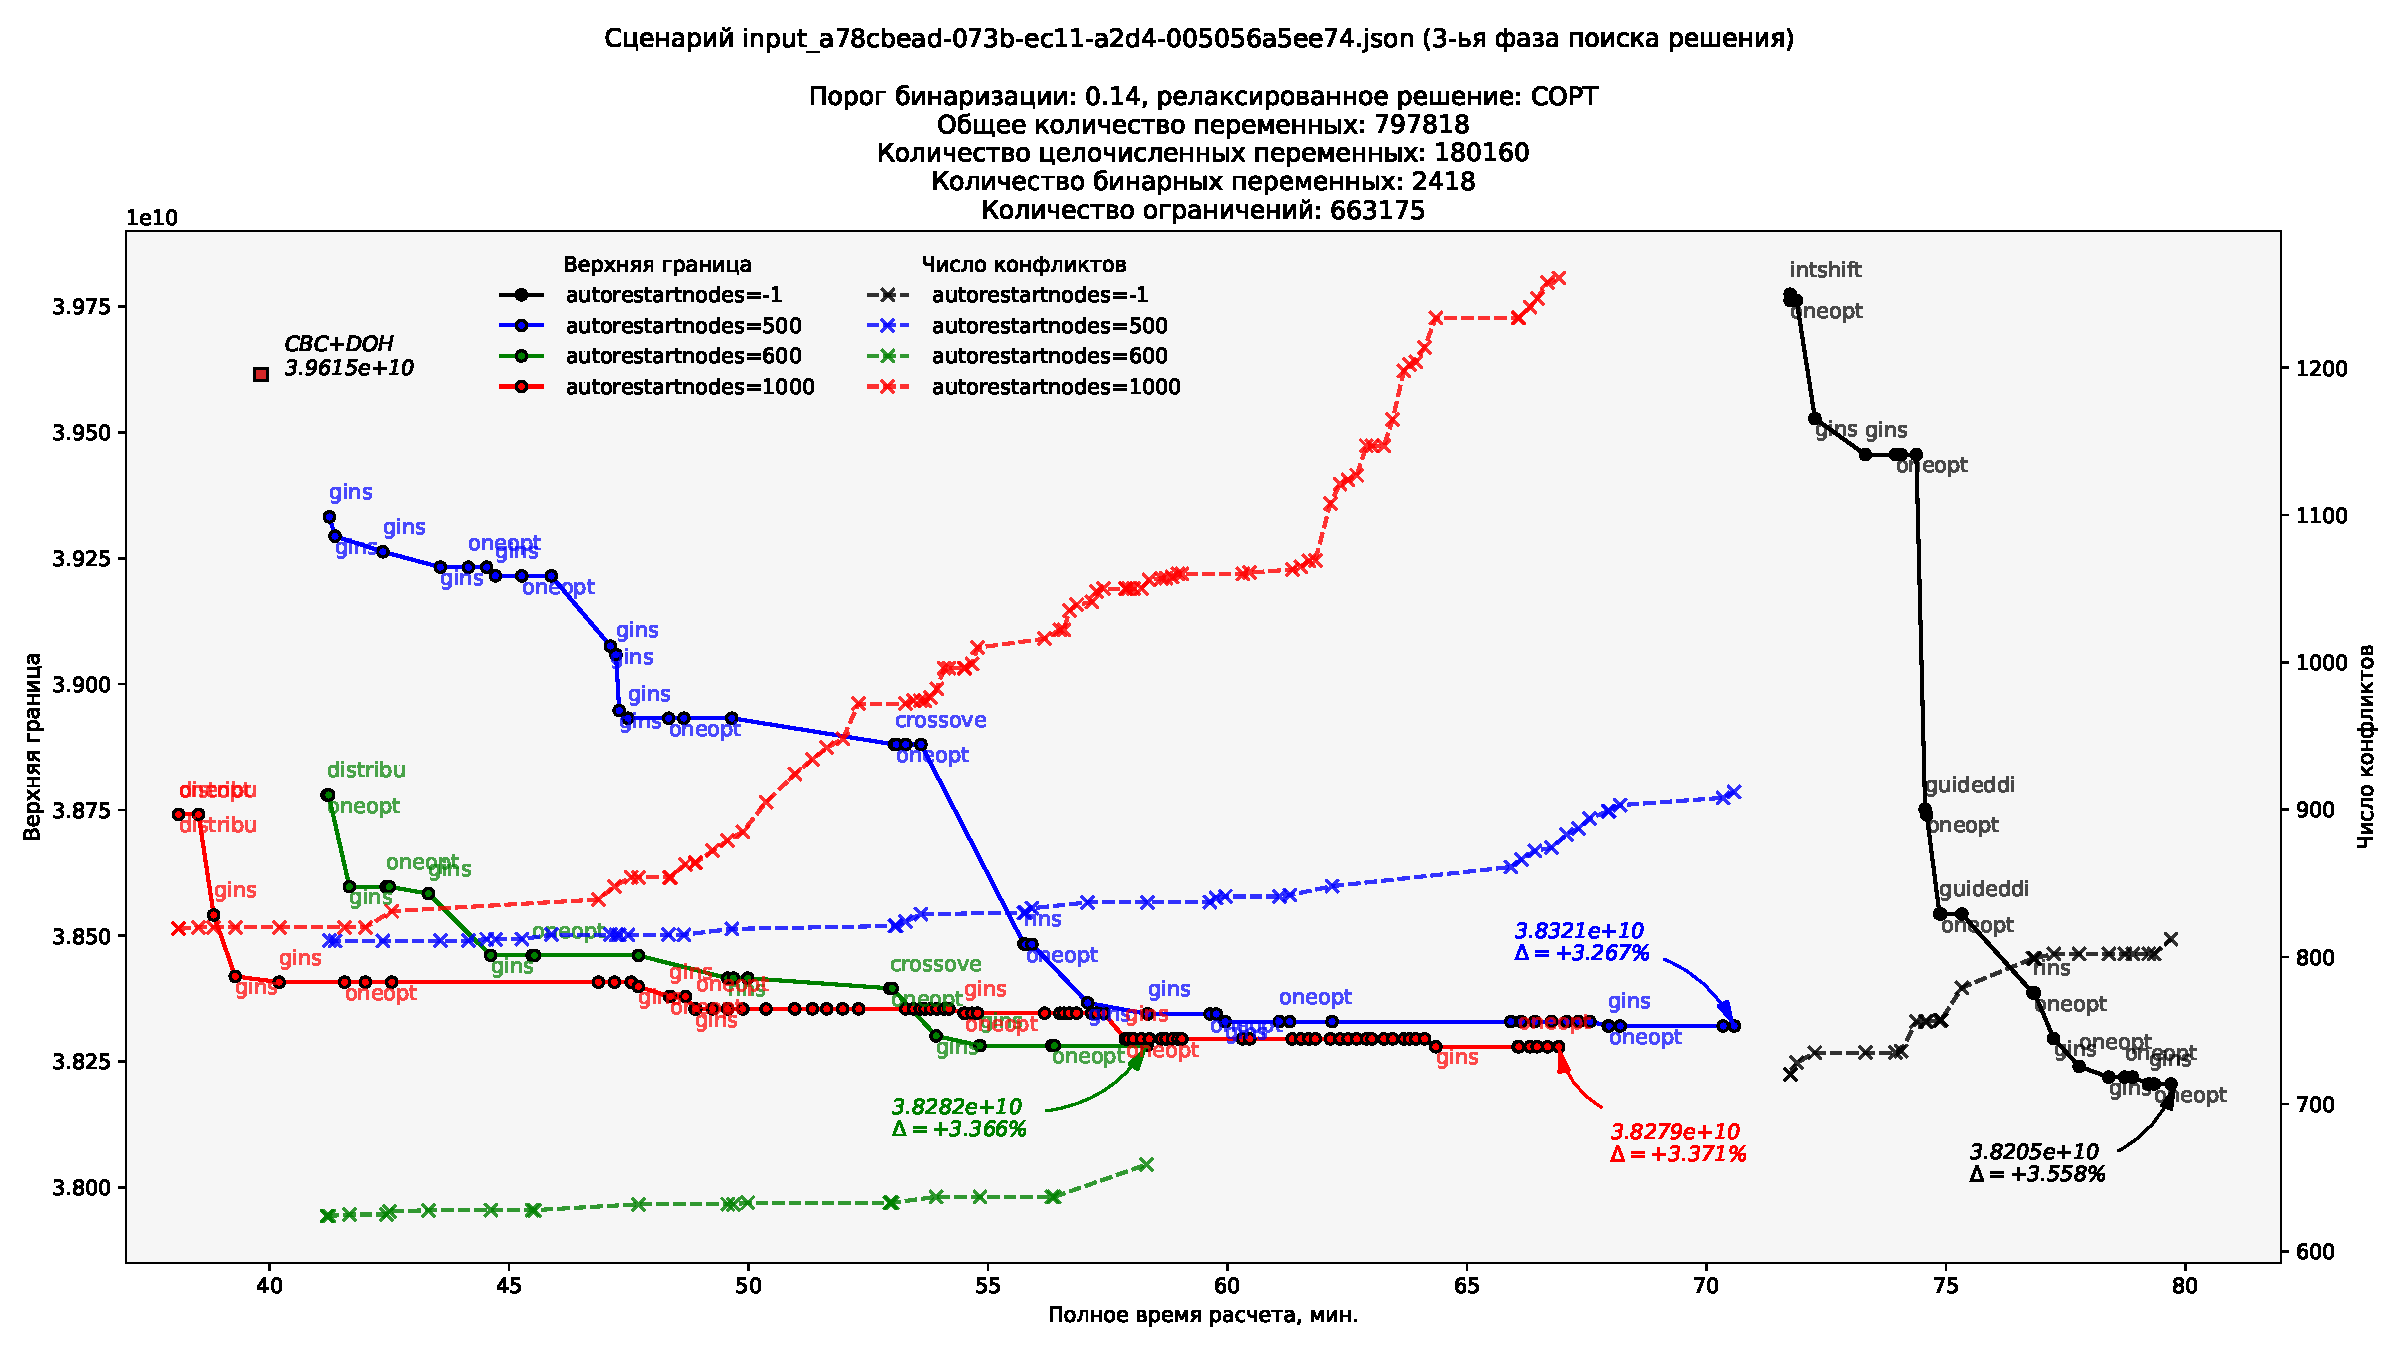
\includegraphics[scale=0.42]{figures/a78cbead_autorestartnodes_3_phase.pdf}
	\caption{ Динамика изменения верхней границы решения и числа конфликтов во времени в зависимости \\от значения параметра \texttt{autorestartnodes}. Сценарий \texttt{a78cbead}. Третья фаза поиска решения }\label{fig:a78cbead_autorestartnodes_3_phase}
\end{figure}
%\end{landscape}

%\begin{landscape}
\begin{figure}[!h]
	\centering
	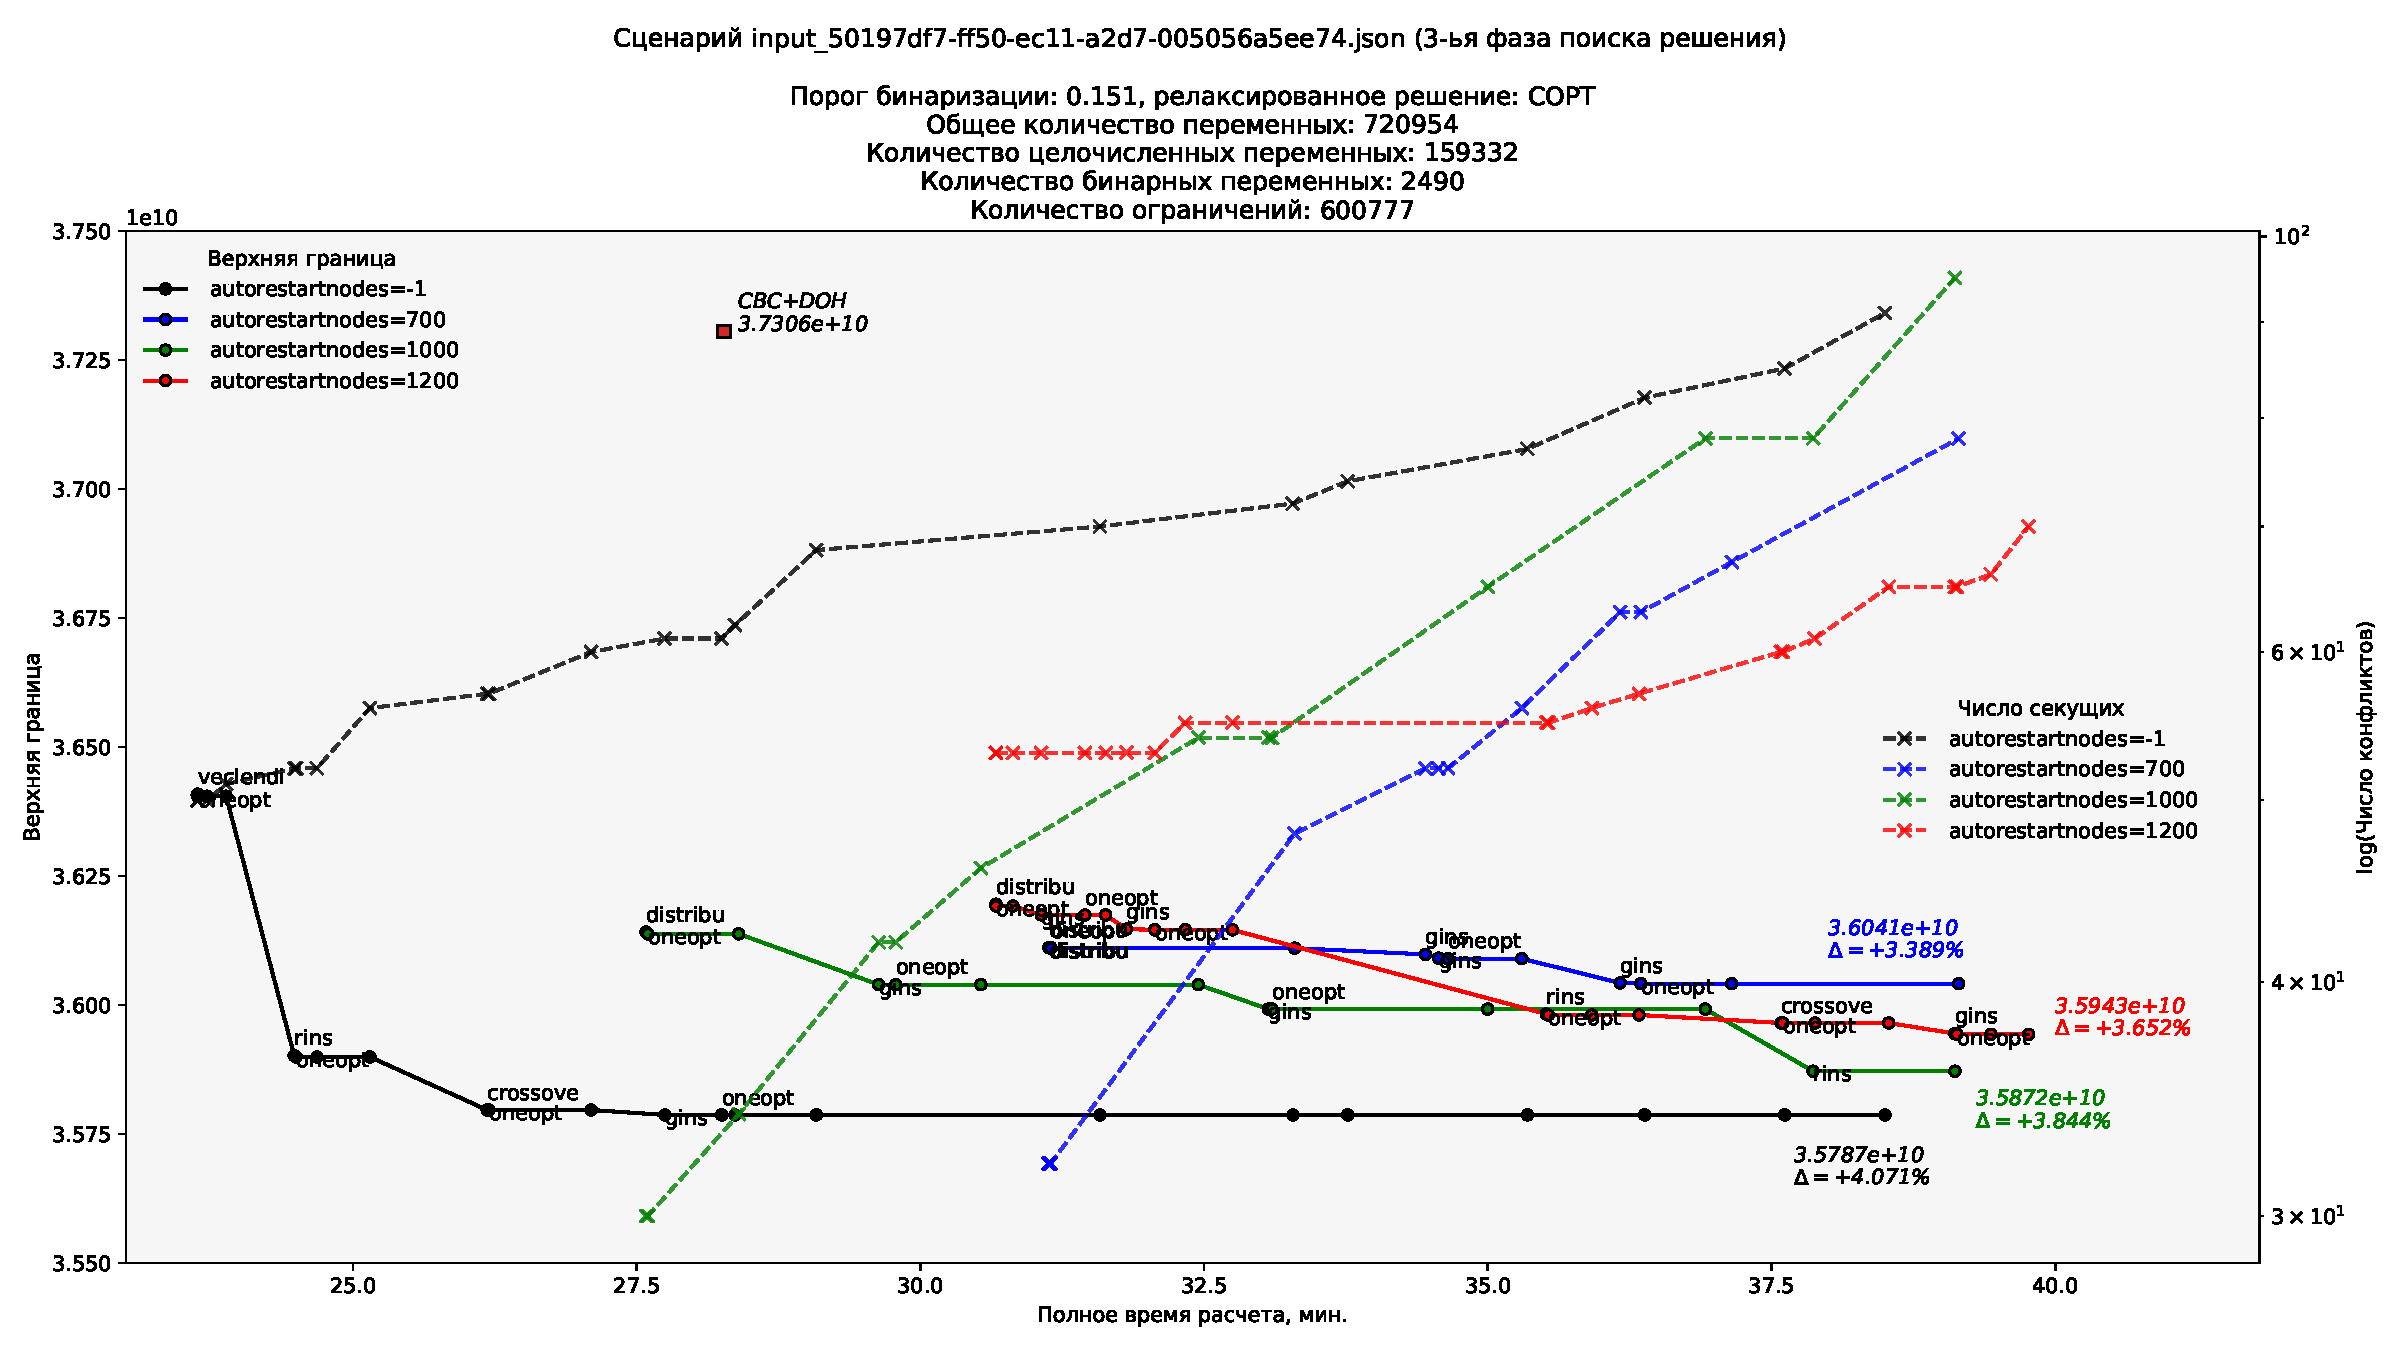
\includegraphics[scale=0.42]{figures/50197df7_autorestartnodes.pdf}
	\caption{ Динамика изменения верхней границы решения и числа конфликтов во времени в зависимости \\от значения параметра \texttt{autorestartnodes}. Сценарий \texttt{50197df7}. Третья фаза поиска решения}\label{fig:50197df7_autorestartnodes}
\end{figure}
%\end{landscape}

%\begin{landscape}
\begin{figure}[!h]
	\centering
	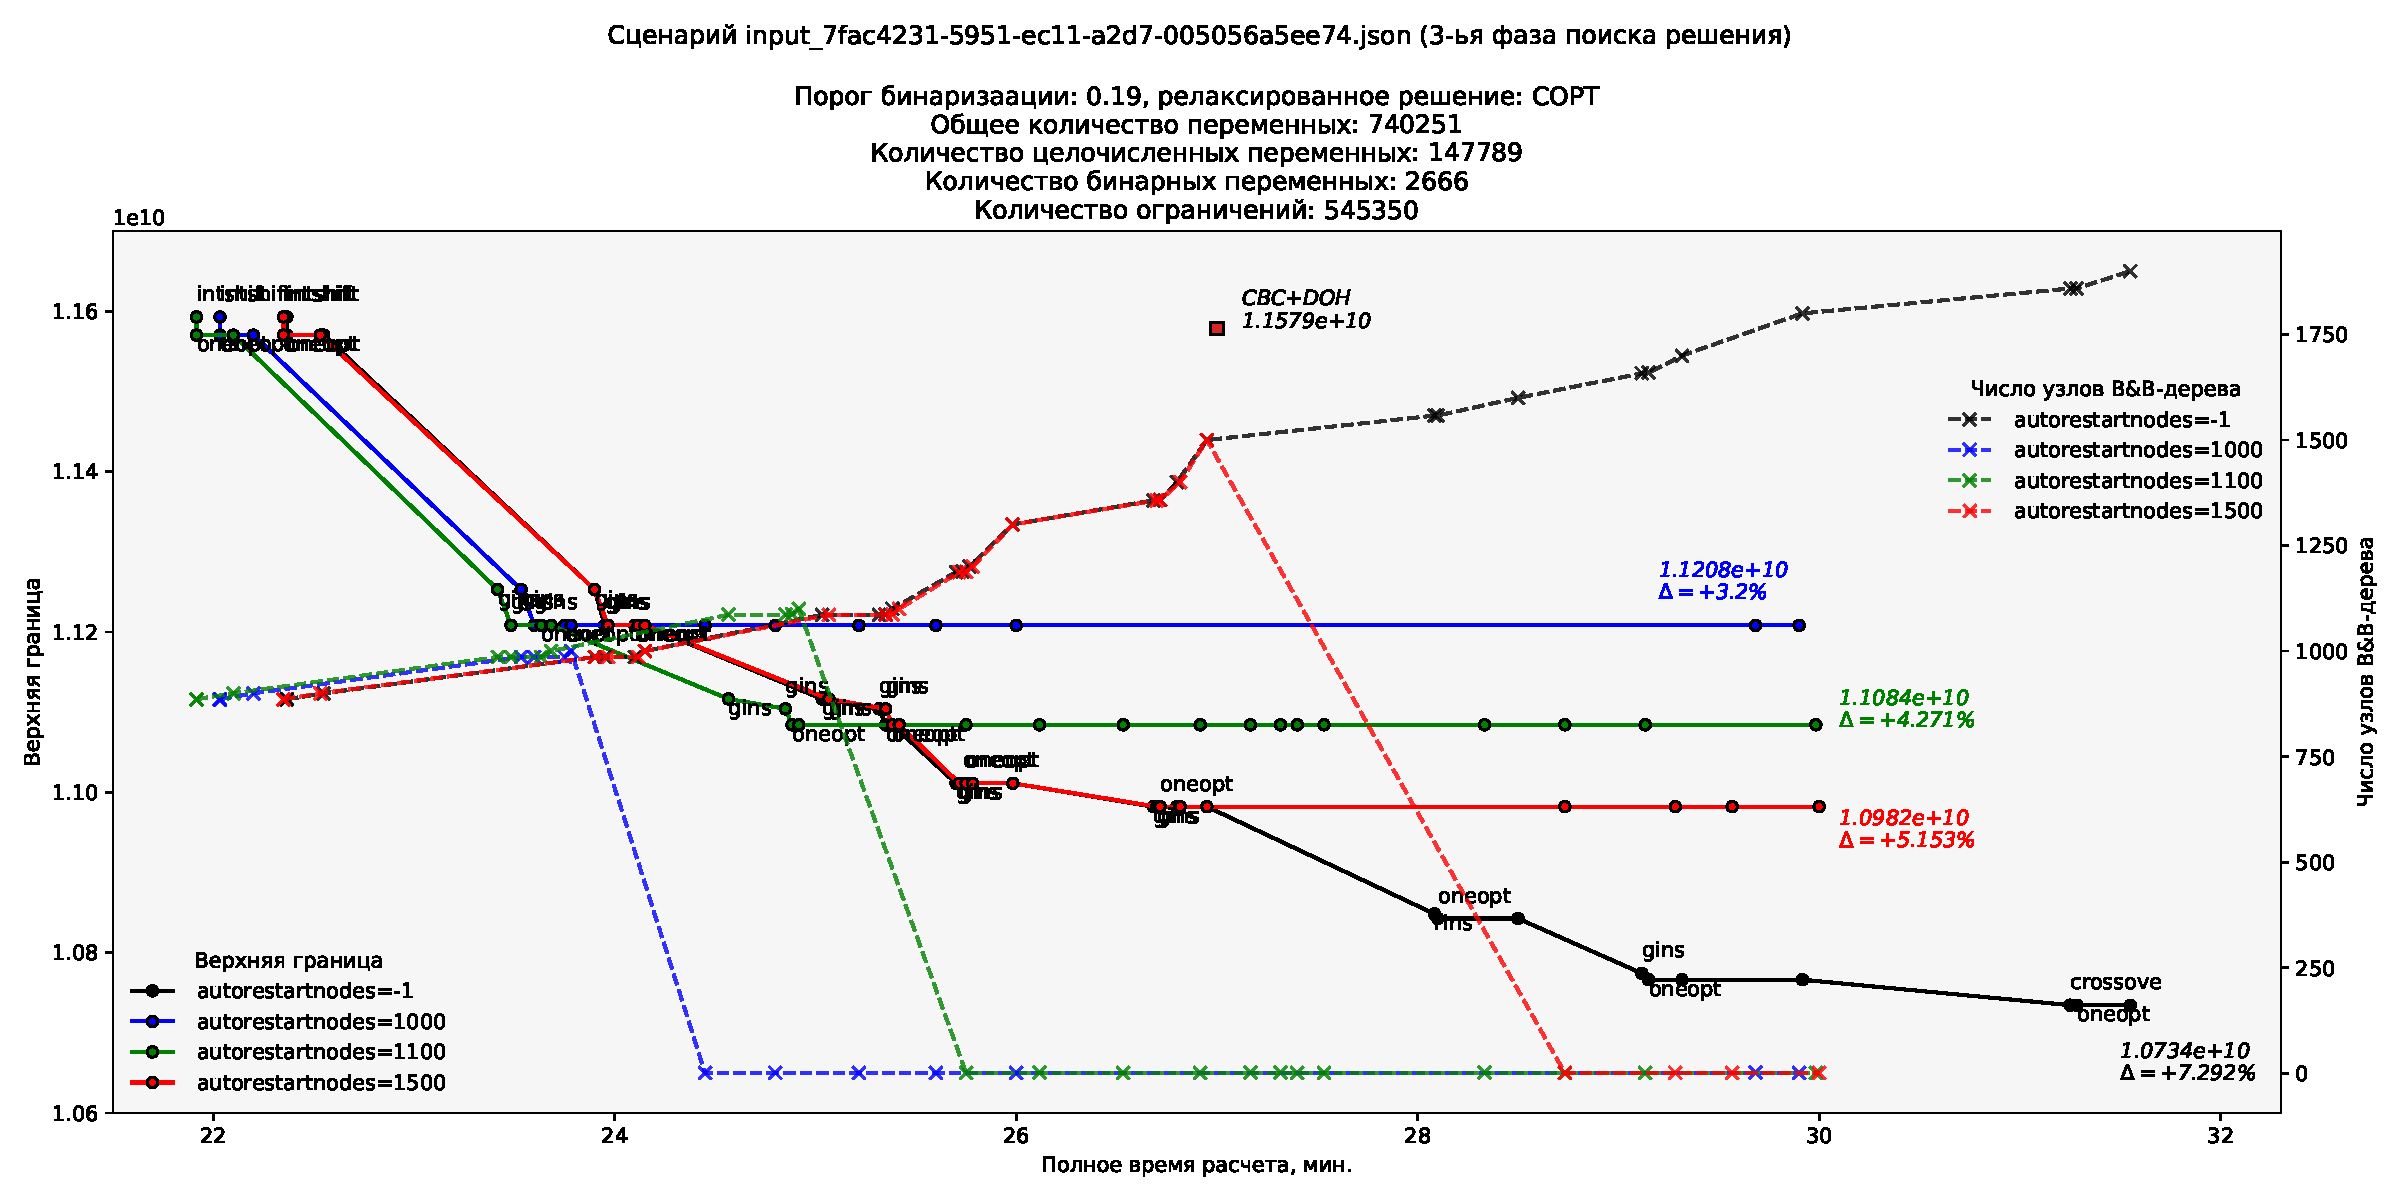
\includegraphics[scale=0.42]{figures/7fac4231_autorestartnodes.pdf}
	\caption{ Динамика изменения верхней границы решения и числа конфликтов во времени в зависимости \\от значения параметра \texttt{autorestartnodes}. Сценарий \texttt{7fac4231}. Третья фаза поиска решения}\label{fig:7fac4231_autorestartnodes}
\end{figure}
%\end{landscape}

\subsection{Поиск решения на базе методов машинного и глубокого обучения}

Условимся \emph{сценарием обучающего поднабора} называть сценарий (математическую постановку задачи, описанную в терманах математического программирования) из коллекции сценариев, которые используются на \emph{обучающей фазе} модели машинного обучения.

\emph{Сценарием тестового поднабора} условимся называть сценарий, который используется \emph{для построения прогноза} с помощью модели машинного обучения.

\subsubsection{Простое декартово произведение сценариев \emph{с} бинарными переменными}

 Рассмотрим \emph{некоммутативные} пары вида <<сценарий обучающего поднабора -- сценарий тестового поднабора>> подгруппы сценариев с бинарными переменными (см. раздел \ref{sec:ikp_bins}):
\begin{itemize}
	\item \texttt{7fac4231\_bin.lp},
	
	\item \texttt{a78cbead\_bin.lp},
	
	\item \texttt{f398266b\_bin.lp},
	
	\item \texttt{50197df7\_bin.lp},
	
	\item \texttt{337\_bin.lp}.
\end{itemize}

Если коллекция сценариев содержит $ n $ сценариев, то существует $ n (n - 1) $ возможных некоммутативных пар.

\paragraph{обучение на сценарии \texttt{7fac4231\_bin.lp}, тестирование на сценарии \texttt{50197df7\_bin.lp}}

...

\paragraph{обучение на сценарии \texttt{a78cbead\_bin.lp}, тестирование на сценарии \texttt{50197df7\_bin.lp}}

...


\paragraph{обучение на сценарии \texttt{f398266b\_bin.lp}, тестирование на сценарии \texttt{50197df7\_bin.lp}}

...


\paragraph{обучение на сценарии \texttt{337\_bin.lp}, тестирование на сценарии \texttt{50197df7\_bin.lp}}

...провал

\paragraph{обучение на сценарии \texttt{7fac4231\_bin.lp}, тестирование на сценарии \texttt{50197df7\_bin.lp}}



\section{Описание вычислительных экспериментов на сценариях группы MBO}

\section{Описание вычислительных экспериментов \\на сценариях MIPLIB~2017}

\subsection{Сценарии со статусом <<open>>}

\subsubsection{Сценарий \texttt{DLR2}}

\url{https://miplib.zib.de/WebData/instances/dlr2.mps.gz}

\subsubsection{Сценарий \texttt{CVRPA-N64K9VRPI}}

\url{https://miplib.zib.de/WebData/instances/cvrpa-n64k9vrpi.mps.gz}

\subsection{Сценарии со статусом <<hard>>}

\subsubsection{Сценарий \texttt{CRYPTANALYSISKB128N5OBJ14}}

\url{https://miplib.zib.de/WebData/instances/cryptanalysiskb128n5obj14.mps.gz}

\subsection{Сценарии со статусом <<easy>>}

\subsubsection{Сценарий \texttt{NEOS-4332801-seret}}

\url{https://miplib.zib.de/WebData/instances/neos-4332801-seret.mps.gz}


\newpage
\listoffigures\addcontentsline{toc}{section}{Список иллюстраций}

\listoftables\addcontentsline{toc}{section}{Список таблиц}

% Источники в "Газовой промышленности" нумеруются по мере упоминания 
\begin{thebibliography}{99}\addcontentsline{toc}{section}{Список литературы}
	\bibitem{ivanov:rl-2022}{\emph{Иванов} Конспект по обучению с подкреплением, 2022}
	
	\bibitem{geron:ml-2018}{\emph{Жерон, О.} Прикладное машинное обучение с помощью Scikit-Learn и TensorFlow: концепции, инструменты и техники для создания интеллектуальных систем. -- СПб.: ООО <<Альфа-книга>>, 2018. -- 688 с.}
	
	\bibitem{soenen:effect-hyper-param-tuning:2021}{\emph{Soenen J. etc.} The Effect of Hyperparameter Tuning on the Comparative Evaluation of Unsupervised Anomaly Detection Methods, 2021}
\end{thebibliography}

\end{document}
